\documentclass[12pt,english]{article}
\usepackage[longnamesfirst]{natbib}
\bibliographystyle{jf}
%\usepackage[T1]{fontenc}
%\usepackage{lmodern}
%\usepackage[T1]{fontenc}
%\usepackage{cmbright}
%\renewcommand\familydefault{\rmdefault}
%\usepackage{unicode-math}
%\usepackage{newcomputermodern}

% times font with libertine math
%\usepackage{mathpazo}
%\usepackage{libertinust1math}
%\usepackage{times}

% Times
%\usepackage[T1]{fontenc}
%\usepackage[utf8]{inputenc}
%\usepackage{mathptmx}


% \usepackage[varg]{txfonts}
%\usepackage{fouriernc}
%\usepackage{stix}

%\usepackage[T1]{fontenc}
%\usepackage{newpxtext,newpxmath}

% times
%\usepackage{fouriernc}
%\usepackage{times}
%\usepackage{newpxmath}

% Libertine
%\usepackage{libertine}
%\usepackage{libertinust1math}
%\usepackage[T1]{fontenc}
%\usepackage{mathpazo}

% Newpx
\usepackage{newpxtext,newpxmath}
\usepackage[T1]{fontenc}

\let\Bbbk\relax
\let\openbox\undefined

\usepackage[bottom]{footmisc}
\usepackage{tabularx}
\usepackage{booktabs}
\usepackage{amsmath,enumerate}
\usepackage{amsthm}
\usepackage{dsfont}
\usepackage{amssymb}
\usepackage{mathtools}
\usepackage{mathrsfs}
\usepackage{graphicx}
\usepackage{natbib}
\usepackage[labelfont=bf,justification=justified,font=footnotesize,skip=2pt,labelsep=period]{caption}
\usepackage{subcaption}
% \usepackage{subfig}
\usepackage{setspace}
\usepackage{arydshln}
\usepackage{chngpage}
\usepackage{float,appendix}
\usepackage{afterpage}
\usepackage{verbatim}
\usepackage{indentfirst}
%\usepackage[margin=1in]{geometry}
\usepackage[left=1in, right=1in, top=1.5in, bottom=1.5in]{geometry}
\usepackage[usenames, dvipsnames]{color}
\usepackage{hyperref}
\usepackage{adjustbox}
% \usepackage{longtable}
\usepackage{booktabs, makecell, longtable,ltxtable}
\usepackage{lipsum}
\usepackage{pdflscape}
\usepackage{siunitx}
\usepackage{chngcntr}
\usepackage{lipsum}
\usepackage{tikz}
\usepackage{pdflscape}
\usepackage[normalem]{ulem}
\usepackage{chngcntr,apptools}
\AtAppendix{\counterwithin{lemma}{section}}
\usepackage{siunitx}
\usepackage{tabularx}
\sisetup{table-format=-1.3, table-space-text-post={**}}
\usepackage{xr}
\usepackage{etoolbox}
\usetikzlibrary{positioning}
\newcommand\fnsep{\textsuperscript{,}}
\usepackage{tikz}
\usepackage{pdflscape}
\usepackage[normalem]{ulem}
\usepackage{chngcntr,apptools}
\AtAppendix{\counterwithin{lemma}{section}}
\usepackage{siunitx}
\usepackage{tabularx}
\usepackage{xr}
\usepackage{etoolbox}
\usetikzlibrary{positioning}
\usetikzlibrary{decorations.pathreplacing}
\usetikzlibrary{calligraphy}
\usepackage[shortlabels]{enumitem}
\usepackage{accents} % for accents
%\MakeRobust{\underaccent} % make \underaccent not fragile in moving arguments
\usepackage{etoolbox}
\robustify{\underaccent}
\usepackage{dutchcal} % \mathcal: also small letters. \mathbcal = bold ones. 
\usepackage{minitoc} % table of contents for just the appendix
%\newcounter{minitocdepth}
%\setcounter{minitocdepth}{5}
\definecolor{UCLAblue}{RGB}{30, 75, 135} % secondary color	
\definecolor{UCLAgold}{RGB}{255, 232, 0} % UCLA Gold
\definecolor{usccardinal}{rgb}{0.6, 0.0, 0.0}
\definecolor{Matlabblue}{rgb}{0,0.447,0.741}
\definecolor{bleudefrance}{rgb}{0.19,0.55, 0.91}
\definecolor{cobalt}{rgb}{0.0, 0.28,0.67}
\definecolor{darkblue}{rgb}{0.0, 0.0,0.55}
\definecolor{darkcerulean}{rgb}{0.03,0.27, 0.49}
\definecolor{darkpowderblue}{rgb}{0.0,0.2, 0.6}
\definecolor{bleudefrance}{rgb}{0.19,0.55, 0.91}
%\usepackage[colorlinks=true,urlcolor=blue,linkcolor=blue,citecolor=blue]{hyperref}


% for arXiv
\hypersetup{colorlinks,allcolors=black}
% pretty blue color for links
%\hypersetup{
%	colorlinks,
%	linkcolor={UCLAblue},
%	citecolor={UCLAblue},
%	urlcolor={UCLAblue},
%}

\bibpunct{(}{)}{;}{a}{,}{,}
% Custom Commands
\newcommand\one{\mathds{1}}
\newcommand\F{\mathcal{F}}
\newcommand\I{\mathcal{I}}
\newcommand\G{\mathcal{G}}
\renewcommand\H{\mathcal{H}}
\newcommand\Z{\mathbb{Z}}
\newcommand\N{\mathbb{N}}
\newcommand\R{\mathbb{R}}
\renewcommand\Pr{\mathbf{P}}
\newcommand\st{\text{ such that }}
\newcommand\Bwoc{By way of contradiction}
\newcommand\Wlog{Without loss of generality}
\newcommand\Var{\mathbb{V}\text{ar}}
\newcommand\Cov{\text{Cov}}
\newcommand\BLP{\text{BLP}}
\renewcommand\implies{\Rightarrow}
\newcommand\E{\mathbb{E}}
\newcommand\plim{\underset{n \to \infty}{\text{plim}}}
%\renewcommand\S{\mathcal{S}}
\newcommand\W{\mathcal{W}}
\newcommand\diag{\text{diag}}
\newcommand\Diag{\text{Diag}}
\newcommand\ntlim{\underset{\substack{N / T = c \\ N,T \to \infty}}{\text{lim}}}
\newcommand\tr{\text{tr}}
\newcommand\toP{\overset{\mathbb{P}}{\to}}
\renewcommand\mod{\;\text{mod}\;}
\renewcommand{\ss}[1]{\scriptscriptstyle{#1}\textstyle}
\newcommand{\udot}[1]{\underaccent{\dot}{#1}}
\newcommand{\Rho}{\mathcal{P}}
\newcommand{\K}{\mathcal{K}}
\newcommand{\kk}{\mathcal{k}}
%\DeclareRobustCommand{\udot}[1]{\underaccent{\dot}{#1}}
\newcommand\grad{\nabla_{z_{k,t}}}
\renewcommand{\partname}{}
\renewcommand{\thepart}{}
\DeclarePairedDelimiter\ceil{\lceil}{\rceil}
\DeclarePairedDelimiter\floor{\lfloor}{\rfloor}
\renewcommand\u{\underline}
\newtheorem{theorem}{Theorem}
\newtheorem{lemma}{Lemma}
\newtheorem{cor}{Corollary}
\newtheorem{prop}{Proposition}
\newtheorem{assum}{Assumption}
\newtheorem{defn}{Definition}
% \newcommand{\E}{\mathbb{E}}
% \newcommand{\var}{\mathrm{Var}}
% \newcommand{\cov}{\mathrm{Cov}}
% \setcounter{MaxMatrixCols}{20}
% \newtheorem{theorem}{Theorem}
% \newtheorem{lemma}{Lemma}
% \newtheorem{defn}{Definition}
% \newtheorem{lesson}{Lesson}
% \newtheorem{prop}{Proposition}
% \newtheorem{cor}{Corollary}
\urlstyle{same}
\usepackage{pgfplots} 
\pgfplotsset{compat=newest} 
\pgfplotsset{plot coordinates/math parser=false} 

%% puts figures and tables at the end of the document
%\usepackage[nomarkers,nolists]{endfloat}               

%% puts ONLY figures at the end of the document
%\usepackage[nomarkers,nolists,figuresonly]{endfloat}  

%% allows more than one figure per page for endfloat
%\renewcommand{\efloatseparator}{\mbox{}}              

\usepackage{rotating}

% allows sideways tables and figures to be placed at the end of the document
%\DeclareDelayedFloatFlavor{sidewaystable}{table}
%\DeclareDelayedFloatFlavor{sidewaysfigure}{figure}

% \usepackage[nomarkers,nolists]{endfloat} 
% \renewcommand{\efloatseparator}{\mbox{}}         % allows more than one figure per page for endfloat

\pgfplotsset{compat=newest} 
\pgfplotsset{plot coordinates/math parser=false} 
\newlength\figureheight 
\newlength\figurewidth 
\usepackage{mathtools}
\usetikzlibrary{calc}

% inverse breve symbol
\usepackage[T3,T1]{fontenc}
\DeclareSymbolFont{tipa}{T3}{cmr}{m}{n}
\DeclareMathAccent{\invbreve}{\mathalpha}{tipa}{16}

% Appendix table of contents
\setcounter{secnumdepth}{4}
\setcounter{tocdepth}{4}
\setcounter{parttocdepth}{4}







 
\usepackage[en-US]{datetime2}
\usepackage{mathtools}
\usepackage{xcolor}




\title{\textbf{The Elasticity of Quantitative Investment}\thanks{I thank Michael Weber, Joachim Freyberger, and Andreas Neuhierl for providing excellent data. I thank Lubos Pastor, Stefan Nagel, Ralph Koijen, and Niels Gormsen, Doug Diamond, Lars Hansen, John Heaton, Anthony Zhang, Bryan Kelly, Toby Moskowitz, Stefano Giglio, James Choi, Christopher Clayton, Paul Goldsmith-Pinkham, Gary Gorton, Song Ma, Elena Asparouhova, Jonathan Brogaard, Davidson Heath, Mark Jansen, Avner Kalay, Yihui Pan, Jiacui Li, Philip Bond, Stephan Siegel, Léa Stern, Christopher Hrdlicka, Yang Song, Adem Atmaz, Huseyin Gulen, Svetlana Bryzgalova, Roberto Gomez Cram, Marco Grotteria, Christopher Hennessy, Victor DeMiguel, Steven Kou, Andrew Lyasoff, Max Reppen, Scott Robertson, Lucy White, Hao Xing, Fernando Zapatero, Christian Heyerdahl-Larsen, Fotis Grigoris, Preetesh Kantak, Fahiz Baba Yara, Craig Holden, Noah Stoffman, Daniel Carvalho, James H. Cardon, Brigham Frandsen, Lars Lefgren, Olga Stoddard, Mark Showalter, Riley Wilson, Brian Boyer, Tyler Shumway, Karl Diether, Ryan Pratt, Craig Merrill, Darren Aiello, Taylor Nadauld and seminar participants at University of Utah, University of Washington, Yale, Purdue, London Business School, Boston University, Brigham Young University Economics Department, Brigham Young University Finance Department and Indiana University for their helpful comments and input. This paper was earlier circulated with the title "Machine Learning, Quantitative Portfolio Choice, and Mispricing."}}
\author{Carter Davis\thanks{Indiana University Kelley School of Business. \href{mailto:ckd1@iu.edu}{ckd1@iu.edu}}}
\date{Original: January 3, 2021 $\;\;\;$ Current: \today}
%\date{\today}
%\date{February 8, 2022}
% Please direct all questions or comment to \href{mailto:carterdavis@chicagobooth.edu}{carterdavis@chicagobooth.edu}.
% \usepackage[hidelinks]{hyperref}

\begin{document}
{\fontfamily{qpl}\selectfont
\doparttoc % Tell to minitoc to generate a toc for the parts
\faketableofcontents % Run a fake tableofcontents command for the partocs
  \sloppy
  \maketitle
  \thispagestyle{empty}

    \begin{abstract}

    What is the price elasticity of demand for canonical portfolio choice methods in financial economics? Twelve models from the literature exhibit strikingly inelastic demand, in contrast to classical models. This is due to the difficulty of trading against price changes in practice, and is consistent with demand elasticity estimates. This provides a novel answer to the inelastic markets hypothesis, raises important concerns for the use of strongly elastic investors in theory models, and quantifies the difficulty of trading against potential mispricing aside from the standard limits to arbitrage frictions. Counterfactual experiments with these demand functions exhibit large and persistent alpha. 
  
  %\begin{abstract}
  %  What happens to mispricing when quantitative statistical arbitrageurs---investors using canonical stochastic discount factor (SDF) models to make portfolio choice decisions---enter the market? This question is addressed with counterfactual experiments using an asset demand system methodology. Mispricing increases or marginally decreases when these models are used to manage capital counterfactually. Empirically, the demand functions implied by twelve SDF models have two key characteristics responsible for these mispricing outcomes: their demand functions align poorly with outstanding alpha and are inelastic. This indicates that it is either quite difficult to eliminate mispricing or there are serious empirical shortfalls in these SDF models.  
    
    \vspace{1mm} % \vspace{10mm}
    \bigskip
    
    \noindent 
    \textsc{\textbf{Keywords}}: price elasticity, demand-based asset pricing, machine learning.%, stochastic discount factor models, portfolio choice. 
  
    \medskip
    \noindent
    \textsc{\textbf{JEL Classification}}: G11, G12, G17.  
  \end{abstract}
	
%\newpage
%\setcounter{page}{1}

%\begin{center}\textbf{Conflict-of-interest disclosure statement}\end{center}

%Carter Davis:

%I have nothing to disclose. 

\newpage
%\onehalfspacing
\doublespacing
\setcounter{page}{1}

How investors react to price changes---the price elasticity of demand---is a central quantity of interest in financial economics \citep{ky}. Indeed, the elasticity of demand is considered a measure of the degree of aggressiveness in trading against mispricing \citep{aggressive}. The elasticity is the inverse of price impact from flows and supply shocks, which means that inelastic demand corresponds to large price impacts of trading flows \citep{GK}. Interestingly, since the elasticity is in terms of percentage changes, an investor who doubles their leverage does not necessarily double their elasticity of demand. Indeed, an investor who doubles their leverage for reasons unrelated to prices does not change their elasticity at all. Thus the elasticity of demand is a measure of aggressive trading separate from leverage. 

Recent work has estimated an average elasticity for individual stocks is in the approximate range of 0.3 to 1.6, implying a price impact from about 0.6\% to 3.3\% from trading flows equal to 1\% of shares outstanding \citep{GK}. This stands in stark contrast to calibrations of classic models resulting in much higher elasticity values, e.g. 6,000 in \cite{petajisto} and the cited 5,000 in \cite{GK}. Even the demand of hedge fund and mutual funds, which include classic statistical arbitrage and smart beta funds \citep{lo:quant, ahmed} that are perhaps most like the high-elasticity investors in these models, is strikingly inelastic compared to these calibrations \citep{ky}. What accounts for this difference? 

The purpose of this paper is to measure the elasticity of reasonable statistical arbitrage strategies based on canonical portfolio choice methods from the academic literature. I consider twelve different canonical portfolio choice models from the literature (e.g., \cite{ff3}; \cite{brandt}; \cite{kelly}; \cite{shrinking}). I calculate not only the portfolio weights that come from these models, but also how these models react to changing prices. The main finding of the paper is that these methods have strikingly inelastic demand. Why is this? In classic models, the only uncertainty comes from not knowing the future realizations of well-known and understood random variables. Many variables in models are often fixed, known, and exogenous to prices, e.g. the covariance matrix of returns, the set of state variables that matter, the structure of equilibrium, and expected asset payouts. For example, \cite{impactinvesting}, \cite{bigdata}, \cite{heaton}, \cite{benchmarking}, \cite{intermediaries}, \cite{kyle85} have assets with expected payouts that are exogenous to prices. Thus when price of the asset changes, there is strong incentive to trade aggressively against the price change since a 1\% decrease in prices represents a 1\% increase in expected returns. These models are then applied the stock market, where stock payouts are the sum of future dividends and prices, and future prices are likely not exogenous to today's prices. \cite{Vuolteenaho/2002} and \cite{goncalves/2021} show that much of the price movements in individual stocks is associated with long-term discount rates and cash flow news, rather than only next-period returns. Thus most price movements have much less than one-for-one predictability for next-period returns. This helps explain the so-called inelastic markets hypothesis, as coined by \cite{GK}. 

The reason that demand for these methods is inelastic can be summarized succinctly: trading against stock-level mispricing is risky and hard.\footnote{If statistical arbitrage is risky, perhaps it should not be called arbitrage. Also, the term statistical arbitrageur is perhaps overly broad, as it includes investment strategies apart from classic factor bets, e.g. pairs trading. However, in the spirit of the literature, e.g. \cite{stein}, I refer to as a hypothetical investor who invests according to these methods as a statistical arbitrageur.} While this concept is not new, quantification of using methods from the literature is novel. In contrast to many classical models, canonical portfolio choice strategies invest according to some method that maximizes an objective function based on some concept of historical performance. While there are certainly fixed inputs into these models, fewer components of the model tend to be exogenous, fixed, and known. In many cases, nearly all components of the investment rules are modeled with uncertainty \citep[e.g.][]{shrinking}. Thus in many classical models with so much held constant, a 1\% price change represents near arbitrage opportunities. With canonical portfolio choice strategies, a 1\% price change is far less predictive of trading profits. Thus these methods have much less elastic demand. 

These demand functions are relatively inelastic because there is so much noise in the time series and cross-section, making it difficult to create a factor model that strongly depends on prices. I document how a 1\% price change effects the standard predictors (often valuation ratios) used in these models. These changes tend to be relatively small, making the portfolio weights relatively insensitive to prices, because it is difficult to construct reliable valuation ratios in the cross-section that are sensitive to prices. Indeed, most portfolio choice models heavily rely on predictors that are not even a function of prices, such as investment and profitability, which makes the models' demand more inelastic. Finally, noise in the time series means that estimates of alpha today are made from historical data, making model-implied demand relatively inelastic. Updating a factor's alpha frequently as a function of prices is difficult since long time periods are needed to estimate this alpha given this time series noise. 

There are two lenses with which to view linear factor models that price the cross-section\footnote{I use the typical definition of a factor model that prices the cross-section: all test assets have zero alpha relative to this model.} and their corresponding linear SDFs:\footnote{Certainly an arbitrary SDF does not necessarily deliver a linear factor model. However, a linear factor model that prices the cross sectional corresponds to a linear SDF \citep{interpreting}.} (1) models that describe the cross-section of returns or (2) investment advice for mean-variance investors.\footnote{A factor model only prices the cross section if and only if it delivers the highest possible Sharpe ratio. See the ``agnostic interpretation" of factor models in \cite{famaprize} that comes from the logic in \cite{hubermankandel}.} The first lens is typically used in academic papers, but certainly the second lens is well-known and understood (e.g., \cite{pastorjmp}; \cite{interpreting}; \cite{brandt}; \cite{demiguel}). 

There is a rich literature that views these models through this second lens. For example, \cite{pastorjmp}, \cite{brandt}, and \cite{demiguel} consider various methods of computing weights on a set of factors from an optimal portfolio choice perspective. \cite{interpreting} think of arbitrageurs who essentially use a factor model to trade against mispricing. Indeed, this is so common in the literature that I refer to these as canonical portfolio choice models. Given this second lens equivalence, these statistical arbitrageur models should produce mean-variance demand functions, meaning that the elasticity should be identical. % For example, \cite{pastorjmp} computes optimal weights on a set of factors from a Bayesian statistical arbitrageur mean-variance investor perspective. \cite{interpreting} think of arbitrageurs who essentially use a factor model to trade against mispricing. \cite{brandt} consider using a set of predictors from classic factor models to produce optimal portfolio choice strategies. \cite{demiguel} compare factor model based investment strategies to see how these strategies perform from an optimal portfolio choice perspective.

Take for example an investor who believes the \cite{ff3} three-factor model prices the cross-section of returns and wants to invest in a portfolio with the highest possible Sharpe ratio (i.e., mean-variance preferences). In this case, the investor believes that instead of diving into the complicated work of investing in many individual assets, the highest Sharpe ratio can be achieved by investing by only using three predictors: (1) market equity, (2) book-to-market ratio, and (3) relative size. These three predictors from this model---in combination with some method such as \cite{pastorjmp}, \cite{demiguel}, or \cite{shrinking} to choose how much to weight each predictor---generates a demand function for individual assets. 

%three portfolios from this factor model. This is what it means for a factor model to price the cross-section: some combination of the factors produces the highest Sharpe ratio portfolio achievable. Thus, in this case, demand for individual stocks will be a function of each stock's (1) market equity, (2) book-to-market ratio, and (3) relative size. I consider this style of statistical arbitrageur demand where weights on these predictors are based on historical returns data (e.g., \cite{pastorjmp}, \cite{demiguel}, \cite{shrinking}). Thus, in this case, the investor uses this canonical factor model---in combination with some method such as \cite{pastorjmp}, \cite{demiguel}, or \cite{shrinking} to choose how much to invest in each of the three portfolios---to actually make investment decisions. This creates a demand function for the individual assets within these factors, which I consider. 

The asset pricing literature has produced a large set of return predictors, also known as asset characteristics. The large set of portfolios formed based on these predictors is often known as the factor zoo and has been discussed at length in the literature \citep{cochrane, harvey, taming}. There are two types of predictors, those that are a direct function of price (e.g. price ratio variables like book-to-market and earnings-to-market) and those that are not a function of price (e.g. \cite{famafrench15} profitability and investment are functions of only accounting variables). In order to calculate the elasticity of a statistical arbitrageur, one must calculate how a 1\% price change affects predictors, and then how changes in those predictors affect the ultimate portfolio weights. I use the \cite{weber} 62 predictors, although some models like \cite{famafrench15} and \cite{zhang} use only a small subset of these predictors. In the literature, often portfolio weights are formed based on discontinuous functions of predictors \citep[e.g.][]{famafrench15}, but to measure these price pass-throughs with derivatives, differentiable approximations of \cite{kelly} and \cite{shrinking} portfolio weight functions are used. 

%There is a well-known equivalence between mean-variance efficient weights, factor models that price the cross-section, and linear SDF models. I define these three concepts carefully in the Appendix and prove their equivalence. Note that in general, an SDF is not equivalent to a linear factor model. Only the type of linear SDF defined in the appendix are equivalent to linear factor models. Because of this equivalence, I refer to (statistical) arbitrageurs, factor models, and portfolio choice methods interchangeably.   %However, due to this equivalence, I use the terms statistical arbitrageurs, SDF models, factor models, mean-variance efficient weights, and canonical portfolio choice methods interchangeably.\footnote{For clarity, I refer to the models how they are usually referenced. For example, I refer to the \cite{ff3} three-factor model (instead of SDF) and the \cite{shrinking} SDF (instead of factor model), since this is the usual way these models are referenced.}

While the very purpose of linear factor models is to describe why different assets earn different returns \citep{kelly}, the discussion of how these models react to changes in prices is strangely sparse in the factor model literature.\footnote{A notable exception is \cite{vanbinsbergenopp}, who show that price wedges and short-term alpha do not have a one-for-one relationship.} The factor model literature is no small niche of the literature either, it is the ``greatest collective endeavor of the asset pricing field in the past 40 years" \citep{kelly}. If a factor model is perfectly inelastic in an extreme case, then the model only describes differences in returns unrelated to prices. A model with a large positive elasticity value implies that the model shifts optimal weights strongly when prices shift, implying the the model is potentially able to describe differences in the cross section that are actually due to prices. A model with a negative elasticity value implies that the model corresponds to momentum-style upward sloping demand. Across the twelve models, there are relatively large quantitative differences. For example, the modified version of the \cite{forest} model is the most elastic model with an elasticity of about 16, while the \cite{kelly} model has an elasticity of about -8. The average elasticity value is across models is 3.4. Importantly, this means this paper introduces a novel and important new concept to the literature: the elasticity of a factor model.

%The portfolio choice demand functions in this paper 
%are a superset of typical agents in economic models (see \cite{learning} for a review). A typical economic agent in the literature knows the true data generating process (DGP), and uses Bayesian learning to update their beliefs. While I consider models with Bayesian learning components or motivation (e.g., \cite{shrinking}), 
%differ from standard theoretical Bayesian statistical arbitrageurs. I consider quantitative investment strategies that take a reasonable quantitative model using a set of return predictors, estimate the parameters, and invest accordingly. In this sense, the arbitrageurs in this paper are like empirically oriented economists in that they make assumptions, estimate a model, and use the parameter estimates to make inferences and decisions. %In fact, these models were created by economists; I consider arbitrageurs that come from the academic literature and are shown to perform well out-of-sample, including \cite{brandt}, \cite{demiguel}, or simply the \cite{ff3} three-factor model.

The elasticity of these factor models is for the most part more elastic than the average elasticity of about 0.3 in \cite{ky}, hereafter just KY, which is perhaps the most commonly referenced estimate of elasticity estimates. However, I show that KY have a relatively restricted functional form. I estimate the demand elasticity using a functional form similar to the flexible factor model demand presented in the paper to determine if this restriction explains the difference in elasticity values. I find that indeed, when demand is estimated with an unrestricted model, the elasticity is higher and comparable to factor model demand. Importantly, the unrestricted demand function aggregates well, meaning that multiple funds with different investment strategies within the same 13F institution have a combined demand function with the same functional form. In KY, the demand is exponential linear in predictors, but the demand function of multiple funds combined is not also exponential linear. \cite{GK} estimate a macroeconomic demand function with similarly good aggregation properties, and this paper contributes to the microeconomics (stock-level) asset demand estimation literature with a demand function with good aggregation properties. 

Once one realizes that (1) many predictors are not a function of stock prices, (2) time-series noise makes predicting real-time alphas difficult, and (3) cross sectional noise makes it difficult to create valuation ratios that move strongly with prices, it is not surprising that these statistical arbitrageurs are inelastic. In an extreme case, an investor who invests according to the CAPM as a market indexer has perfectly inelastic demand, which is well-known \citep{ky}. If the result is not surprising, why does this matter? One can interpret this inelastic demand in one of two ways. First, to the degree to which these statistical arbitrageurs represent actual hedge funds and mutual funds who use smart beta or other statistical arbitrage techniques in practice, this shows that these investors cannot actually invest aggressively against mispricing as many models imply. This exercise quantifies an important limit to arbitrage apart from the fear of losing investments under management \citep{limitsarb}, correlated arbitrage capital \citep{cho}, or a host of other limits \citep{stein}. To be clear, many other limits to arbitrage translate into lower price elasticity values, but the model-implied elasticity values are low for reasons separate than this broad literature. These are essentially friction-free models, but the fundamental risk still implies low elasticity values. %There is a vast chasm between the classic model elasticity of 7,000 calibrated below and those in the literature. Explaining this with only a mix of classically elastic investors and market indexers requires 

Second, to the degree that these models do not represent actual statistical arbitrage investors in practice, this result is still an important contribution to the factor model and cross sectional asset pricing literature. Given recent the elasticity estimates in this paper, KY, and the rest of the literature surveyed in \cite{GK}, actual statistical arbitrageurs likely do not have more elastic demand than these models. Thus these models provide an upper bound on a reasonable degree to which statistical arbitrageurs have the capacity to trade against price movements, even before imposing common literature frictions \citep[e.g.][]{limitsarb}. Note that the framework of these models is relatively general: the models simply use a broad set of predictors, many based on prices, to produce optimal portfolio weights. This is much more general than just showing that market indexers are inelastic, this shows that by leveraging the vast set of return predictors from the literature using twelve models honed to combine these predictors optimally, even the most price-sensitive models fall far short of classical elasticity values of 5,000. While it is perhaps unsurprising that these models deliver inelastic demand, it is striking how well these elasticity values line up with estimated elasticity values than for example, the midpoint of this vast range between 5,000 and the estimated values. The elasticity provides a useful metric for factor models that answers the question: how sensitive is this model to asset prices? This provides an important contribution to the large cross sectional asset pricing literature \citep[e.g.][]{harvey, taming, cochrane, shrinking}. This paper also provides a critique for theoretical models that contain highly elastic investors, and rely on these investors to rule out mispricing or create small price impacts from flows. Thus this paper contributes to the literature on limits to arbitrage, \citep[e.g.][]{limitsarb, cho, interpreting, bigdata, fama:disagreement:tastes, hartkreps, stein, hongstein}. %Also, any failure of academic models to represent optimal statistical arbitrage models reflects on the ability of these models to price the cross section. 

% This is a vast range between the classic model elasticity of 5,000 and those in the literature.

%Assume, for the sake of argument, that actual statistical arbitrageurs are able to deliver much higher Sharpe ratios than those shown in this paper, with potentially very different methods. This would fundamentally call into question the validity of this large set of models. A factor model only prices the cross if and only if it delivers the highest possible Sharpe ratio.\footnote{See the ``agnostic interpretation" of factor models in \cite{famaprize} that comes from the logic in \cite{hubermankandel}.} Thus a failure of academic models to represent optimal statistical arbitrage models directly reflects a failure on the part of these models and the directly related effort to develop a model to describe the cross section of returns. 

At the end of the paper, I show counterfactual experiments with the statistical arbitrage demand from these models combined with estimated demand. Following KY, the counterfactual experiments hold fixed shares outstanding and accounting variables, and determine what the historical price of all individual stocks in the sample with counterfactual insertions of the statistical arbitrageur models in this paper. Interestingly, CAPM alpha in some cases increases in magnitude and is never eliminated. This is unsurprising given the levered but inelastic demand of these models, but lends some credence to the idea that trading against prices and statistical arbitrage in the stock market is difficult. 

\section{Elasticity of Theoretical Statistical Arbitrageurs} \label{sec:elasticity}

In order to discuss the elasticity of statistical arbitrage, we first have to explore the elasticity of standard theoretical model-based investors. 

Consider a set of $N$ assets. Suppose an arbitrageur has $a$ assets under management.\footnote{If this is a household instead, then $a$ would denote the wealth of the household.} Let $p_i$ denote the share price of asset $i$, and $w_i$ denote the portfolio weight of the fund for the asset. Then $s_i = a w_i / p_i$ denotes the number of shares of the asset that the fund owns. The elasticity is defined as:
\begin{equation} \label{eq:elasticity}
    \eta_{i} \equiv - \frac{\partial \log (s_i)}{\partial \log (p_i)} = 1 - \frac{\partial \log(w_i)}{\partial \log (p_i)}
\end{equation}
where in calculating the second equation, I follow KY by assuming the assets under management are exogenous.\footnote{In other words, the assumption is
\begin{equation*}
    \frac{\partial \log(a)}{\partial \log (p_i)} = 0. 
\end{equation*}
This assumption is problematic in a macroeconomics setting where the market-level return is being examined. This paper focuses on the microeconomics cross-sectional setting, where this assumption is less problematic. } For example, an elasticity of 3.5 implies that a 1\% increase in the price would lead to a 3.5\% decrease in the shares demanded for the asset. 

As KY point out, value-weighted index funds are designed to avoid rebalancing for price fluctuations, and are thus perfectly inelastic. This can be seen using equation (\ref{eq:elasticity}), since a 1\% price rise leads to a 1\% increase in the asset's portfolio weights. Thus, $\partial \log (w_i) / \partial \log(p_i) = 1$, and $\eta_i = 0$ ($=1-1$).\footnote{As shown below, static models with classic mean-variance demand have very elastic demand. It is this type of model that is typically used to derive the CAPM. However, if one believes the CAPM and then because of this just invests in the market without paying attention to prices, then this investor has completely inelastic demand. As this becomes more widespread, aggregate demand strikingly becomes more inelastic. This is analogous to the famous \cite{grossman:stiglitz} paradox, rephrased in terms of elasticity. }

The price elasticity is a key quantity in asset pricing models, because it describes how investors react to price changes. If investor demand strongly reacts to price changes, then the effect of many behavioral biases can be either dampened or entirely offset (see \cite{GK} for a discussion on the importance of demand elasticity). Demand elasticity is also the inverse of the price impact of investment flows. Thus, inelastic demand implies a large price impact. 

%I next give a simple numeric example for the implied price elasticity from a constant absolute risk aversion (CARA) utility model of many assets. Then I outline why factor model investing would yield more inelastic demand relative to the CARA utility demand function. 
The point of this section is not to convince the reader that statistical arbitrageurs produce inelastic demand. This is shown empirically below for the twelve models in this paper. This section simply (1) points out that these elasticity values are quite low relative to their theoretical counterpart and (2) gives some basic reasoning with a simple model for why statistical arbitrageur demand is inelastic. 

\subsection{Elasticity of Classic Models: A Simple Calibration Exercise}

Consider an investor with CARA utility that chooses a vector of portfolio weights $w_t$ at time $t$ of the $N$ risky assets. Let $r_{t}$ be the vector of returns in excess of the risk-free rate, with the gross risk-free rate $R_{f,t}$. The investor chooses $w_t$ to maximize utility:
\begin{equation}
    \E_t \left[ -\exp \left( -\gamma a_t (w_t' r_{t+1} + R_{f,t}) \right) \right]
\end{equation}
where $\gamma$ is the CARA risk-aversion coefficient and $\iota$ is a vector of ones. The classic demand, with multivariate normal returns, is then:
\begin{equation}
    w_t = \frac{1}{\gamma a_t} \Sigma_t^{-1} \mu_t
\end{equation}
where $\Sigma_t = \Var (r_{t+1})$ is the $N \times N$ covariance matrix, $\mu_t = \E_t [r_{t+1}]$ is the vector of expected excess returns. 

Alternatively, consider the case of Epstein-Zin multivariate demand for the $N$ risky assets from \cite{campbell:chan:viceira}. Let $y_{t}$ be the $N$ dimensional vector of log returns minus the log risk-free return. They show,
 after log-linearization, portfolio weights are given by the approximation:
\begin{equation} \label{eq:ez_weights}
    w_t = \frac{1}{\tilde \gamma} \tilde \Sigma_t^{-1} \left[ \tilde \mu_{t} + \frac{1}{2} \sigma_t^2 - \frac{\theta}{\psi} \sigma_{c-w,t} \right],
\end{equation}
where $\tilde \mu_t = \E_t [y_{t+1}]$, $\tilde \Sigma_t$ is the $N \times N$ conditional covariance matrix of $y_{t+1}$, $\sigma_t^2$ is the $N$ dimensional vector containing the diagonal elements of $\tilde \Sigma_t$, $\sigma_{c-w,t}$ is the $N$ dimensional vector of conditional covariance of the log consumption to wealth ratio and $y_{t+1}$, $\tilde \gamma > 0$ is the relative risk aversion coefficient, $\psi > 0$ is the elasticity of intertemporal substitution, and $\theta \equiv (1 - \tilde \gamma) / (1 - \psi^{-1})$.\footnote{See equation (20) of \cite{campbell:chan:viceira}. Note that in their equation, there are some additional terms because they also consider $y_t$ to be log return of the asset minus a benchmark with potential covariance terms. We consider just the risk-free rate, which eliminates some of these extra terms.} Recall that Epstein-Zin demand nests CRRA demand. 

It is common to have a covariance matrix that is exogenous to prices. It is also quite common, across a large variety of models, to model assets with expected payouts that are exogenous to prices \citep[e.g.][]{impactinvesting, bigdata, heaton, benchmarking, intermediaries, kyle85}.\footnote{For example, \cite{impactinvesting} have a ``liquidating dividend" at the end of the single period, and it is easy to see that this expected payoff is exogenous to prices. This is extremely common in asset pricing models, but then the model-implied price impact (inverse of demand elasticity) is sometimes used to assess the actual impact of investment flows (e.g. ESG investment in this example).}\footnote{One may argue that in equilibrium, prices cannot move independently from payoffs in some of these models. This argument misses the definition of the elasticity of demand, which is calculated based on the demand function before prices are solved for in equilibrium. Indeed, in many models prices can move very little precisely because demand is elastic and therefore price impact from flows is small. Price elasticity is not defined by trades, it is defined as the sensitivity of a demand function to price movements, even if those price movements are off-equilibrium price movements. Indeed there is a demand price elasticity even in a model with a representative investor.} Many of these models are applied to stock markets. Given the two demand functions above, with exogenous covariance matrices and expected asset payouts, the only other way that prices can affect demand other than through expected returns ($\mu_t$ or $\tilde \mu_t$), is through the consumption-to-wealth covariance term $\sigma_{c-w,t}$ in Epstein-Zin demand. \cite{whyinelastic} show that empirically, this consumption-to-wealth component affects elasticity values only slightly.\footnote{This is sensible economically as well, since the consumption to wealth ratio is an aggregate quantity, and thus a 1\% price change does not appear to affect the covariance of individual asset returns and the consumption to wealth ratio. In \cite{whyinelastic}, at the largest, this term decreases the elasticity value by at most 6\% of the total elasticity value. Even 94\% of the calibrated elasticity value is orders of magnitude above literature estimates.} Thus ignoring this hedging component in calculating the elasticity, we can use the chain rule to expand equation (\ref{eq:elasticity}):
\begin{equation} \label{eq:eta_mu}
    \eta_{i,t} = 1 - \frac{\partial w_{i,t}}{\partial \mu_{i,t}} \frac{1}{w_{i,t}} \frac{\partial \mu_{i,t}}{\partial \log (p_{i,t})},
\end{equation}
where we can write this same equation, but replace $\mu_{i,t}$ with $\tilde \mu_{i,t}$ as well. 

Let $\chi_{i,t+1}$ be the exogenous payoff. With this payoff, we can calculate:
\begin{equation}
    \frac{\partial \mu_{i,t}}{\partial \log (p_{i,t})}
    = \frac{\partial}{\partial \log (p_{i,t})} \left( \frac{\E_t[\chi_{i,t+1}]}{\exp ( \log (p_{i,t}))} - R_{f,t} \right) = -(\mu_{i,t} + R_{f,t}) \text{ and }
\end{equation}
\begin{equation}
    \frac{\partial \tilde \mu_{i,t}}{\partial \log (p_{i,t})}
    = \frac{\partial}{\partial \log (p_{i,t})} \left( \E_t [\log (\chi_{i,t+1})] - \log (p_{i,t}) - \log (R_{f,t}) \right) = -1.
\end{equation}
Assuming $\mu_{i,t} + R_{f,t} > 1$, then we can use $-1$ as a conservative approximation for both of these derivatives in the elasticity equation. \cite{whyinelastic} criticize this feature of many models (i.e. $\partial \tilde \mu_{i,t} / \partial \log (p_{i,t}) = -1$), in particular static models, and how this is often used to generate unrealistically small price impacts and high elasticity values. Plugging this into equation (\ref{eq:eta_mu}) yields:
\begin{equation}
    \eta_{i,t} = 1 + \frac{\partial w_{i,t}}{\partial \mu_{i,t}} \frac{1}{w_{i,t}},
\end{equation}
which we can again write as a function of $\tilde \mu_{i,t}$ for the Epstein-Zin case. 

Note that any increase (decrease) in $\gamma a_t$ or $\tilde \gamma$ decreases (increases) $\partial w_{i,t} / \partial \mu_{i,t}$ or $\partial w_{i,t} / \partial \tilde \mu_{i,t}$ respectively by the exactly the same amount that $1 / w_{i,t}$ increases (decreases) by. Thus elasticity values are independent of any positively chosen $\gamma a_t$ or $\tilde \gamma$, and thus without loss of generality with regard to elasticity calculations, we can set these parameters such that the weights of risky assets sum to one in equilibrium.\footnote{This is consistent with a zero net supply of the risk-free asset, which is again assumed without loss of generality in regards to elasticity value calculations. Given the parameter values below, this is set at $a_t \gamma = \tilde \gamma = 2.2$. }

To show the magnitude of this elasticity, I plug in a set of parameters. I consider $N = $ 1,000 assets, and consider an asset with an average portfolio weights, i.e. $w_{i,t} = 1 / N$.\footnote{This does not mean this calibration only holds for equally weighted portfolios. It simply means we consider an asset with an average portfolio weight.} I set the correlation between all stocks to be 0.3,\footnote{\cite{pollet} report average daily correlations to be 0.237, and longer-horizon correlations are higher due to autocorrelations across days. Thus, I use 0.3 as a reasonable parameter value} a volatility of 30\% per annum, an expected excess return of individual stocks to be 6\%. This implies $\partial w_{i,t} / \partial \mu_{i,t} \approx 7.2$ in the case of CARA demand. This delivers an elasticity of about 7,000 ($\approx 1 + 1000 \times 7.2$). This is comparable to the elasticity value of 6,000 from \cite{petajisto}, and similar to \cite{GK}, which cites an elasticity of 5,000 or above in classical models. To calibrate the Epstein-Zin demand elasticity, with a similar covariance structure and assuming the term $\tilde \mu_{t} + \frac{1}{2} \sigma_t^2 - \frac{\theta}{\psi} \sigma_{c-w,t}$ is about 6\%, then this of course delivers the same demand elasticity. 

When the elasticity is written in this form, as $\eta_i = 1 + N (\partial w_{i,t} / \partial \mu_{i,t})$, with many assets and reasonable values of expected returns and covariances, it is clear that the elasticity is likely to be at least three orders of magnitude larger than unity (similar to \cite{petajisto}). This exercise also reveals how standard multivariate utility yields much higher elasticity values than in settings with only a single or a few assets. This is intuitive, since many assets naturally means that assets will be better substitutes for each other and thus have a higher price elasticity, while a setting with only a single or a few risky assets naturally provides only limited substitutability and thus a lower elasticity. 

An elasticity of 7,000 implies that a 1\% drop in prices leads to an 7,000\% increase in shares demanded. This sensitivity to prices is an important component of many asset pricing models. An investor with highly elastic demand has a strong sense of the "right" price. When prices deviate from this price, highly elastic investors trade aggressively against these price deviations. This strong sense of the right price is fundamental to the logic that if there were mispricing, investors would act dramatically in this highly elastic fashion to correct the mispricing. 

What causes this difference in demand elasticity values? What is {wrong} with this calibration? The logic is simple: it is hard to know what the true alpha is and therefore it is hard to know the right price. Alpha is typically assessed using historical data, and thus as prices move, it may be difficult to update the contemporaneous alpha and thus the current mispricing. The calibration {holds all else equal} (e.g., holding risks and expectations of future payoffs equal) and just varies prices, but in practice this is quite hard to do. Empirical canonical portfolio choice models by design try to limit risk while achieving high Sharpe ratios. This risk-return optimization means these models are less inclined to make large bets about the right price---meaning they are relatively inelastic---than their theoretical counterparts that {hold all else equal}. 

For example, it is difficult to determine the alpha of value stocks. Over a two year period (April 2020 - March 2022),\footnote{When the data were downloaded, this was the most recent two-year period.} the long-short portfolio from the \cite{ff3} three-factor model beat the market, after a decade (April 2010 - March 2020) of underperformance. Calculating the CAPM alpha with 5-, 10-, 20-, and 30-year rolling windows yields very different results about the sign and magnitude of the alpha.\footnote{This is well-known, but is also shown in Figure \ref{fig:value_alpha} in the Appendix.} It of course gets more complicated if standard errors are calculated with different assumptions. Is the true value alpha positive, negative, or zero? If the price of value stocks changes quickly, what is the alpha going forward? These questions are inherently challenging. If this was easy, then there likely would not be so much debate over the right factor model. 
% \footnote{The monthly factor returns data were downloaded from Kenneth French's website.}

Due to the difficulty of determining the right price, a statistical arbitrageur that takes a strong stand on the "right" price may make strong levered bets in the wrong direction, which is unlikely to yield a high Sharpe ratio. Thus, the statistical arbitrageurs are actually fairly insensitive to current mispricing. In other words, the statistical arbitrageurs are relatively price inelastic compared to the calibration. In conclusion, this inelasticity is a feature of these statistical arbitrageurs and not a bug. 

\section{Why is Statistical Arbitrageur Investment Inelastic?}

To understand why canonical portfolio choice demand may be relatively inelastic, it is important to first understand the structure of demand from these models. Figure \ref{fig:demand} shows how these demand functions work. The price of a share of stock $i$ in period $t$ is $p_{i,t}$. Various predictors, $x_{i,k,t}$, are a function of this price term. In this example, book-to-market and earnings-to-price ratios are a function of the stock price. However, \cite{famafrench15} profitability is not a function of the price. The $x_{i,k,t}$ raw predictors are transformed into normalized predictors, $z_{i,k,t}$, as described below. Finally, the portfolio weight for stock $i$ is a function of the normalized $z_{i,k,t}$ predictors. This is the general form for KY demand, as well as canonical portfolio methods. 

\begin{figure}[!t] \centering
    \resizebox{0.9\textwidth}{!}{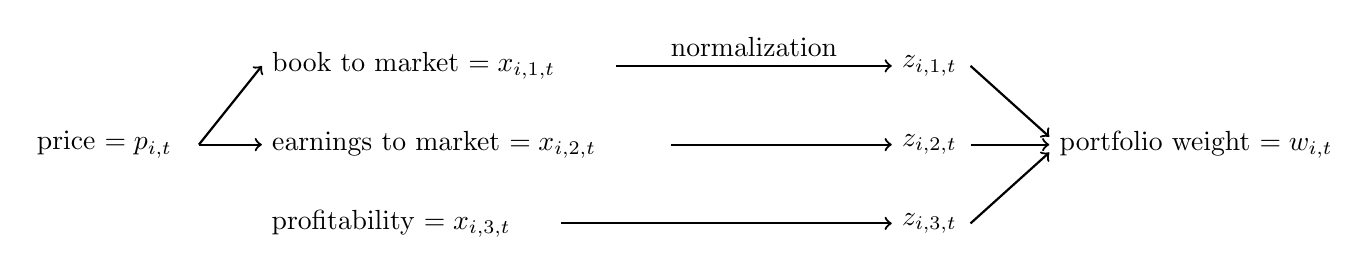
\begin{tikzpicture}
\node[text centered] at (0,0) {price $= p_{i,t}$};
\draw[->,thick] (1.2, 0) -- (2, 1) node [right] {book to market $= x_{i,1,t}$};
\draw[->,thick] (1.2, 0) -- (2, 0) node [right] {earnings to market $= x_{i,2,t}$};
\node[align=left] at (2,-1) [right] {profitability $= x_{i,3,t}$};
%\draw[->, thick] (1.2, 0) -- (2, -1);
%\node[text centered, red, rotate=135] at (1.6, -0.5) {\large X};
\draw[->,thick] (6.5, 1) -- (10, 1) node [right] {$z_{i,1,t}$};
\node[text centered, above] at (8.25, 1) {normalization};
\draw[->,thick] (7.2, 0) -- (10, 0) node [right] {$z_{i,2,t}$};
\draw[->,thick] (5.8, -1) -- (10, -1) node [right] {$z_{i,3,t}$};
\draw[->,thick] (11, 1) -- (12, 0.1);
\draw[->,thick] (11, 0) -- (12, 0) node [right] {portfolio weight $= w_{i,t}$};
\draw[->,thick] (11, -1) -- (12, -0.1);
\end{tikzpicture}}
    \vspace{4mm}
    \caption{\textbf{Demand Mapping.} This figure shows how demand, for statistical arbitrageurs, is a function of prices and predictors. The price of stock $i$ in month $t$ is $p_{i,t}$. In this example, the three predictors used are: (1) the book-to-market ratio, (2) the earnings-to-market ratio, and (3) the profitability ratio. Importantly, the \cite{famafrench15} definition of profitability is not a function of prices, so there is no arrow between prices and profitability. The predictors are mapped into the normalized assets predictors, $z_{i,k,t}$. Then portfolio weights are formed as function of these normalized predictors. }
    \label{fig:demand}
\end{figure}

There are two ways these functions can be modified to create more elastic demand:
\begin{enumerate}
    \item First, the portfolio weights on the factors themselves could be modified to vary substantially with the overall price of the value portfolio. However, as discussed above, it is difficult to determine the current alpha of these factors in real time. In other words, this is difficult because \textit{the time series of factor returns is noisy}. 
    \item Second, the portfolio weights of individual component assets could be modified to vary more with prices. This is difficult as well, because these predictors are only weak signals about future returns on average, and much less so at the individual stock level. In other words, this is difficult because there is so much noise \textit{in the cross-section of individual stock returns}. 
\end{enumerate}

\noindent This does not imply that modifying demand to be more elastic is impossible, just difficult. %In fact, something in the vein of \cite{factortiming} could potentially produce an SDF with more elastic demand, although producing demand in the range of 15,000 is difficult. However, it is clear that canonical portfolio choice models are relatively inelastic and that this matters for mispricing. 
%Thinking of ways of producing SDF demand that is more elastic is beyond the scope of this paper. 

\subsection{Stylized Model}

I consider the case where a mean-variance investor believes that the market and value factor from the \cite{ff3} model price the cross-section of returns, and are thus mean-variance efficient. I exclude the size factor from \cite{ff3} for simplicity. The purpose of this subsection is not to present a general model, but to transparently reveal the key economic reason why the canonical statistical arbitrageurs in this paper are inelastic with as simple a model as possible. 

What is the economic reason that this model produces inelastic demand? In other words, why is this model unsure of the "right" price? This is because book-to-market ratios are noisy unreliable signals about what price should be. The aggregate value premium has at times been historically high (see Figure \ref{fig:value_alpha}), but has fluctuated much through time. Critically, there is even more noise at the individual stock level, meaning that the model is designed such that only relatively large price movements are needed to switch a stock from a value stock to a growth stock, or vice versa. Thus, since large price movements are needed to change asset demand substantially, this statistical arbitrageur has inelastic demand. 

I consider a single asset $i$, which is contained in both the market fund and the value fund. In other words, I consider a market portfolio (composed of many assets), a long-short value portfolio (composed of many assets), and one asset in particular that is potentially in both the market and value portfolios. I will discuss two kinds of portfolio weights: (1) portfolio weights of the factors themselves and (2) portfolio weights of assets within those factors. 

The number of shares outstanding has no economic significance, and thus I assume that there is one share outstanding for the asset considered here\footnote{Investors can invest with fractional shares.}. Let $p_i$ denote the price of this asset, which is the same as market equity if this asset is a stock because there is only one share outstanding. 

Importantly, in this example, each statistical arbitrageur invests a fixed fraction $w$ of her money into the value fund and $1 - w$ into the market. The variable $w$ is {chosen by considering optimal portfolio weights in the data} and critically {does not vary as prices change}. \cite{brandt} and \cite{shrinking} are portfolio optimization methods where the {investment weights for each portfolio do not vary as prices change.} 

The weight of the asset in the market portfolio is $p_i / A$, where $A$ is the value of the market---i.e. $A$ is the sum of the prices of all assets. Assume that the statistical arbitrageur has $\udot{A}$ dollars to invest. Both $A$ and $\udot{A}$ are exogenous. Assume that the asset's weight in the value fund is $u(p_i) p_i / A$, where $u(p_i)$ is a function that equals either 1, 0, or $-1$ depending on whether the asset is in the long portion of the portfolio sort (i.e. $u(p_i) = 1$), the asset has no weight in the portfolio (i.e. $u(p_i) = 0$), or the asset is in the short portion of the portfolio sort (i.e. $u(p_i) = -1$). Notice that this portfolio is a difference of value-weighted portfolios. In other words, this is a standard valued-weighted long-short portfolio. 

In this case, this statistical arbitrageur invests the following amount of dollars into the asset:
\begin{equation*}
    (1 - w) \udot{A} \frac{p_i}{A} + w \udot{A} \frac{u(p_i) p_i}{A}
\end{equation*}
where the first term represents the dollar amount invested in this asset {because the asset is in the market portfolio} and the second term represents the dollar amount investment in this asset {because the asset is in the value portfolio}.

Thus, shares demanded of this asset are:
\begin{equation*}
    s_i = \frac{1}{p_i} \left( (1 - w) \udot{A} \frac{p_i}{A} + w \udot{A} \frac{u(p_i) p_i}{A} \right) = (1 - w) \frac{\udot{A}}{A} + w \udot{A} \frac{u(p_i)}{A}
\end{equation*}
and the elasticity is
\begin{equation*}
    \eta_i = - w \frac{\udot{A}}{s_i} \frac{p_i}{A} \frac{\partial u(p_i)}{\partial p_i}
\end{equation*}

Notice that except for a few portfolio sort break points where the derivative is not defined, $\partial u(p_i) / \partial p_i = 0$. Thus, except for these break points, demand is complete inelastic---i.e. $\eta_i = 0$. This is perhaps not fair to traditional discontinuous portfolio sort methods because demand does change with changes in the price at these break-points. I consider a continuous version of this below. 

It is important to note that if this strategy instead was a combination of investing in the market and a profitability portfolio for example, then $u(p_i)$ would not vary with prices, because market equity does not affect profitability portfolio sorts. In other words, in this example, this demand function is {perfectly inelastic} everywhere. 

Thus, this key result, that the classic quantitative portfolio choice strategies results in relatively inelastic demand almost everywhere holds for any combination of the market portfolio and long-short value-weight portfolios where two conditions hold: (1) portfolio weights of the factors are determined with historical data and not a function of today's fluctuations and (2) large price changes are needed to substantially change the individual asset portfolio weights within the long-short value fund. 

\subsubsection{Continuous Predictors Weighting Instead of Discontinuous Jumps} 

The above $u$ function is characterized by a few discontinuous jumps. Suppose instead, that this $u$ function is linearized. Assume that $p_i$ is known to fall between some small price $p_L$---a low price that makes the asset an extreme value stock---and some large price $p_U$---a high price that makes the asset an extreme growth stock. Assume $p_U - p_L$ is large, which means that the plausible range for $p_i$ is large and the difference between a large growth price and a small value price is large. Define $u$ to be
\begin{equation*}
    u(p_i) = 2 \frac{p_U - p_i}{p_U - p_L} - 1
\end{equation*}

This linearized version of $u(\cdot)$ represents a portfolio that is {predictor-weighted}, like \cite{brandt} and \cite{shrinking}. In other words, the asset in the portfolio is weighted by the degree to which the asset is a value stock or a growth stock.

In this case the elasticity is given by
\begin{equation*}
    \eta_i = 2 w \frac{\udot{A}}{s_i} \frac{p_i}{A} \frac{p_U}{p_U - p_L}
\end{equation*}
Since the growth price $p_U$ is much larger than the value price $p_L$, this quantity is small. Thus, even in this linearized case, statistical arbitrageur demand is still relatively price inelastic. This also nicely shows that if only small changes in prices are needed to move an asset from the long end to the short end of the portfolio---i.e. $p_U - p_L$ is small---then demand can be much more elastic. 

Thus, the key intuition of this subsection is {not} the fact that discontinuous portfolio sorts generate inelastic demand, but rather that statistical arbitrageur demand even with continuous portfolio weights is by design, relatively inelastic. 







\section{Data} \label{sec:data}

I describe the data in this section. First, I describe the Center for Research in Security Prices (CRSP) fund flows data. Then I describe the holdings data, followed by the returns and predictors data. 

The CRSP monthly fund flows data start January 1960 and end March of 2022. I merge these data with the standard market portfolio excess return and risk-free rate data from Kenneth French's website. The risk-free rate is the standard one-month Treasury bill rate. 

I also use quarterly institutional long-only holdings data from the SEC 13F filings dataset. See KY for more details about these data. My sample period is from 1984 to 2020. Across many assets, the 13F holdings often do not account for the entire set of shares outstanding, and I follow KY by creating an additional "household" investor that holds the residual shares.\footnote{This residual investor is labeled "households" by KY.}

I use the monthly equity returns and stock predictors data from \cite{weber}, which contains 62 predictors (i.e. asset characteristics). %Table XXX lists the 62 predictors used, 
A thorough description of the variables can be found at \cite{weber}. This data was extended from 2014 to the end of 2020 by \cite{babayara}. The sample starts in July of 1967. The 13F filing data are are merged with the predictors data. This data is merged to the CRSP monthly returns data which contains changes in shares outstanding, returns, and dividends.

\section{Measuring the Elasticity of Quantitative Investment} \label{sec:elas_models}

\subsection{Notation and Data Preparation}

Let $P_{i,t}$ denote the market equity of stock $i$ at time $t$, while $p_{i,t}$ denotes the share price of the asset. Therefore, $P_{i,t} = S_{i,t} p_{i,t}$ where $S_{i,t}$ denotes the number of shares outstanding. 

I take the raw predictor $k$ for stock $i$ at time $t$, denoted $x_{i,k,t}$, and normalize them as shown in Figure \ref{fig:demand}. For example, $x_{i,k,t}$ could be the book-to-market or profitability ratio in \cite{weber}. As \cite{shrinking} and \cite{kelly} discuss, it is important to normalize the predictor into a well-behaved predictor, $z_{i,k,t}$, for statistical arbitrageurs. 

The main type of normalized predictor is used for the factor models, denoted as $\udot{z}_{i,k,t}$. I use a continuous version of the normalization that \cite{shrinking} and \cite{kelly} use, among others. Their normalization is the raw predictor, $x_{i,k,t}$, mapped into cross-sectional percentiles (between 0 and 1) minus one half (with a resulting range between $-0.5$ and $0.5$). For example, if an asset has a book-to-market ratio in the twentieth percentile in the cross-section of assets, then the resulting normalized value would be $-0.3$ ($= 0.2 - 0.5$). A slightly modified version of these normalized predictors are used in the demand estimation section, which is discussed below. 

I use a continuous version of this percentile transformation, as defined and discussed below. I use a continuous transformation to be able to calculate the elasticity of demand of these statistical arbitrageurs. In other words, every step between prices and portfolio weights in Figure \ref{fig:demand} should be continuous, including having $\udot{z}_{i,k,t}$ be a continuous function of $x_{i,k,t}$. This allows the calculation of $\partial \udot{z}_{i,k,t} / \partial \log (p_{i,t})$ for each predictor (see Appendix \ref{subsec:kernel} for the closed-form formula for these derivatives). 

%Why use these normalized predictors $\udot{z}_{i,k,t}$ instead of just the raw predictors $x_{i,k,t}$? \cite{shrinking} and \cite{kelly} discuss this in detail. Importantly, I follow these authors in using {predictor-weighted} portfolios, as discussed more below. 

The transformation of the raw predictors, $x_{i,k,t}$, into the normalized predictors, $\udot{z}_{i,k,t}$, allows me to form predictor-weighted portfolios. As \cite{shrinking} and \cite{kelly} discuss, using portfolios weighted with these cross-sectional percentiles produces clean long-short portfolios with a long tradition in asset pricing, while using portfolios based on raw predictors, $x_{i,k,t}$, is full of noise. 

\subsection{Continuous Transformation Into Normalized Predictors}

This subsection explains the statistical arbitrageur predictors, denoted as $\udot{z}_{i,k,t}$. I consider the standard predictor-weighted portfolios, like \cite{shrinking} and \cite{kelly}, among others. These are portfolios which are weighted, in the long and short tails of the portfolio, by the cross-sectional deviation of a specific predictor, such as book-to-market or investment values. When using predictors in this way, predictor normalization is critical to producing relatively reliable statistical arbitrageurs \citep[see][]{shrinking}. This alleviates issues with outliers and noise in the data. I discuss the normalization immediately below.

Let $x_{k,t}$ be the $N$-dimensional vector of the raw predictor $k$ known at time $t$ that is filled with the raw predictor $x_{i,k,t}$ values. Let $\udot{z}_{k,t}$ and $\udot{z}_{i,k,t}$ be the corresponding normalized predictors. The standard normalization, used for example in \cite{shrinking} and \cite{kelly}, is to transform the raw predictors to be
\begin{equation}
    \udot{z}_{i,k,t} = \frac{\text{rank} (x_{k,t})_i-1}{N-1} - 0.5 
\end{equation}
where $\text{rank}(\cdot)$ is a function that reads in a vector and outputs a vector of values $1$ through $N$ corresponding to the relative rank of the input values ($N$ is assigned the largest value, $1$ the smallest), and $\text{rank}(\cdot)_i$ is the $i^{th}$ element of this output vector. This transforms predictors to be in the range of $[-0.5, 0.5]$. 

This is a discontinuous function of the predictor $x_{i,k,t}$. If $x_{i,k,t}$ is the book-to-market ratio for example, then any demand function that is a function of $x_{i,k,t}$ is then a discontinuous function of the price. This complicates elasticity estimations. Thus, I create a continuous version of this normalization defined as
\begin{equation} \label{eq:z_weights}
    \udot{z}_{i,k,t} = \K(\text{ArcSinh} (x_{k,t}))_i - 0.5
\end{equation}
where $\text{ArcSinh} (\cdot)$ is the standard inverse hyperbolic sine function and $\K(\cdot)$ is the cumulative distribution function (cdf) of a standard kernel density function. Similar to above, $\K(\cdot)_i$ is the $i^{th}$ element of $\K(\cdot)$. I use the standard well-known normal cdf kernel function, described in detail in Appendix \ref{subsec:kernel} below. 

This transformation above yields very similar results to its discontinuous version, but this function is of course continuous. The $\text{ArcSinh} (\cdot)$ function is used because it is similar to the log function in that it shrinks extreme values towards zero, but $\text{ArcSinh} (\cdot)$ is defined at zero and negative input values.\footnote{In fact, the approximation $\text{ArcSinh} (x) \approx \log(x) + \log(2)$ holds for large values of $x$.} Since many predictors can assume negative values, this is necessary. The final kernel minus one half function is necessary to transform the value into the $[-0.5, 0.5]$ interval. 

\subsection{Forming Linear Predictor-Based Factor Portfolios}

The BPZ$_L$, BSV, DGU, and the KNS models use linear predictor-weighted portfolios, defined here. Following \cite{shrinking}, I rescale these predictors in every period to avoid leverage in the predictor-weighted portfolios from fluctuating across time with the number of assets available. Note that the sum of the absolute value of the predictors in any given period is about $N / 4$ (i.e., $\sum_{i=1}^N | \udot{z}_{i,k,t} | \approx N / 4$).\footnote{Note that $N$ could be notated as $N_t$, since the number of available stocks varies across months. However, to avoid conflicts with standard notation used in \cite{kelly} and \cite{shrinking}, among many others, I use the simpler $N$ term.} For any $x$, I define $\breve x \equiv (4 x) / N$ and $\invbreve x \equiv (N x) / 4$. Thus, I can write $\sum_{i=1}^N | \breve{\udot{z}}_{i,k,t} | \approx 1$. This allows me to define predictor-weighted portfolio returns. Let $F_{k,t+1}^c$ be the zero-cost portfolio return associated with predictor $k$:\footnote{Note that these are zero-cost portfolios even if the weights were all positive because $r_{i,t+1}$ are excess returns, not just returns. However, since the weights, before being scaled down, fall evenly between $-0.5$ and $0.5$ (i.e., weights sum to zero), these are classic long-short predictor weighted portfolios (see \cite{shrinking}).} 
\begin{equation} \label{eq:port_returns}
F_{k,t+1}^c = \sum_{i=1}^N \breve{\udot{z}}_{i,k,t} r_{i,t+1}.
\end{equation}

Factor models, such as \cite{ff3}, require a market portfolio return as well. Let $A_t^j$ be the AUM of institution $j$, and $A_t \equiv \sum_j A_t^j$.\footnote{Note that by this definition, $A_t = \sum_{i} P_{i,t}$. As in KY and discussed below, a residual institution is added so that institutions collectively hold all assets in the data. } I let the first predictor, $k = 1$, be a market portfolio return weight: $\udot{z}_{i,1,t} \equiv \invbreve P_{i,t} / A_t$. Note that this is defined in terms of $\invbreve P_{i,t}$ and not $P_{i,t}$, so that $\sum_{i=1}^N | \breve{\udot{z}}_{i,1,t} | \approx 1$, which matches the other portfolios.

\subsection{Two Types of Predictors}

Following KY, I separate predictors into two categories: (1) those that are a function of price and (2) those where price is not needed or used to calculate the predictor. I follow KY by assuming this latter type of predictors are exogenous to prices, such as historical beta, book values, asset values, investment, and profitability. %Neither share prices nor market capitalization are used when calculating these predictors. 
Fifteen out of the 62 predictors are a function of price. In Appendix \ref{subsec:endogenous}, I describe the classification of the predictors into these two types in more detail. %These 15 endogenous predictors are shown in Table \ref{tab:gradz}, and described in more detail in the Appendix. The Appendix describes the classification of the predictors into endogenous and exogenous predictors.  

Some of the predictors from the \cite{weber} data use historical prices, instead of contemporaneous prices, to create price ratio variables. For example, the book-to-market ratio is computed with stale market capitalization values in order to better match the period when when the accounting book values were released. I follow KY by instead using the most recent prices to calculate these standard valuation ratios. Using historical prices instead of current prices of course would make the statistical arbitrageurs in this paper even less price elastic. However, this seems to violate the spirit of standard valuation ratios. Basing investment decisions on valuation ratios should make investors sensitive to prices, which is why I use contemporaneous prices. As is standard with the CRSP data, the monthly price is the closing price on the last trading day of the month. 

The most difficult predictors to sort into these two categories is the maximum daily return over the previous month and momentum. The maximum daily return is sometimes a function of today's price if the maximum daily return was the most recent day. However, if this is classified into the category of being a function of price, then this is a discontinuous function. Since this is a historical daily flow and not a stock, this classification has little effect on the measured elasticity. Similarly, short term reversals are classified as being a function of price, but momentum is not. Momentum is defined as the return over the past year excluding the most recent month. This means it is not a function of price, while short term reversals are a function of price given that it is the return over the previous month. If these variables are dropped from the dataset, I have similar measured elasticity results. I keep these variables in the data because it is simple, does not change the elasticity results significantly, and keeps the set of predictors the same as \cite{weber}. 

\subsection{Price Sensitivity of Individual Factor Investment}
Table \ref{tab:gradz} shows the 15 endogenous predictors, and importantly the median $\partial \udot{z}_{i,k,t} / \partial \log (p_{i,t})$ derivatives values for each predictor $k$ across assets and months. Some predictors with the price in the numerator, like Tobin's q, tend to have a positive derivative. Other predictors, like the book-to-market ratio, have a price term in the denominator; thus, when the price increases, the predictor tends to decline (negative derivative). A derivative of $-0.25$, for example, means that a 1\% rise in the price implies the predictor decreases by a quarter of its full range (recall the full range of these predictors is between $-0.5$ and $0.5$). The 47 exogenous predictors of course have zero derivatives. 

Note that many of these values are less than one in absolute value. For example, the median book-to-market (beme) derivative is $-0.374$. This is because the log book to market ratio has a relatively large range of values, and it thus needs to be compressed to be in the standard percentile range. The return over the past month (cum\_return\_1\_0) and relative price to high price ratio (rel\_to\_high\_price) values tend to have a relatively small range, and thus need to be expanded in some sense to be transformed into a percentile. This means these values tend to be larger than one in absolute value. 

\begin{table}[!t] \centering
    \resizebox{1.\textwidth}{!}{\begin{tabular}{@{\extracolsep{4pt}}lcc@{\hskip 7.5mm}lcc@{\hskip 7.5mm}lc}
% \\[-1.8ex]\hline
% \hline \\[-1.8ex]
\toprule
 & $\frac{\partial \udot{z}_{i,k,t}}{\partial \log (p_{i,t})}$
 & & &  $\frac{\partial \udot{z}_{i,k,t}}{\partial \log (p_{i,t})}$
 & & & $\frac{\partial \udot{z}_{i,k,t}}{\partial \log (p_{i,t})}$ \\
\\[-1.8ex]
\cline{2-2} \cline{5-5} \cline{8-8}\\[-1.8ex]
Covariates & Gradient & & Covariates & Gradient & & Covariates & Gradient \\
\hline \\[-1.8ex]
a2me &  $-0.273$  & & e2p &  $-0.248$  & & o2p &  $-0.125$ \\
 & ($-0.422$,  $-0.082$) & &  & ($-0.534$,  $0.056$) & &  & ($-0.275$,  $-0.000$)\\
\\[-1.8ex]
beme &  $-0.374$  & & ldp &  $<10^{-10}$  & & q &  $0.321$ \\
 & ($-0.551$,  $-0.083$) & &  & ($-0.296$,  $-0.000$) & &  & ($0.076$,  $0.833$)\\
\\[-1.8ex]
beme\_adj &  $-0.343$  & & lme &  $0.147$  & & rel\_to\_high\_price &  $1.28$ \\
 & ($-0.691$,  $-0.064$) & &  & ($0.057$,  $0.184$) & &  & ($0.287$,  $3.070$)\\
\\[-1.8ex]
cum\_return\_1\_0 &  $2.93$  & & lme\_adj &  $0.037$  & & roc &  $0.161$ \\
 & ($0.504$,  $5.114$) & &  & ($0.003$,  $0.192$) & &  & ($0.019$,  $0.662$)\\
\\[-1.8ex]
debt2p &  $-0.174$  & & nop &  $-0.061$  & & s2p &  $-0.274$ \\
 & ($-0.258$,  $-0.000$) & &  & ($-0.248$,  $0.072$) & &  & ($-0.389$,  $-0.062$)\\
\hline \\[-1.8ex]
 Obs. &  1,869,963 & & & 1,869,963 & & & 1,869,963 \\
 Months & 703 & & & 703 & & & 703 \\
% \hline
% \hline \\[-1.8ex]
\bottomrule
\end{tabular}}
    \vspace{4mm}
    \caption{\textbf{Predictor Price Sensitivity.} This table shows the median (across assets and months) values of $\partial \udot{z}_{i,k,t} / \partial \log (p_{i,t})$---how much the predictor changes when the price of the asset increases by 1\%. %For example, if prices rise by 1\%, the median asset-to-market-equity ratio (a2me) tends to decreases by 0.273. 
    In parentheses under the median values, the 10\% and 90\% percentile of the distribution is reported (this is not a confidence interval of an estimate---the mean has a much smaller variance than the underlying distribution). The variable labels and descriptions are found in \cite{weber}, but I describe them briefly here: a2me is the asset to market equity ratio, beme is the book-to-market ratio, beme\_adj is the book-to-market ratio minus the industry mean, cum\_return\_1\_0 is the return over the previous month (short term reversals variable), debt2p is the debt to price ratio, e2p is the earnings to price ratio, ldp is the dividend to price ratio, lme is market equity (size variable), lme\_adj is the market equity minus industry market equity, nop is the net payout (dividends and net issuance) to price ratio, o2p is the payout (dividends and a different measure of buybacks) to price ratio, q is Tobin's q, rel\_to\_high\_price is the price to 52 week high stock price ratio, roc is an economic rents over cash ratio, and s2p is the sales to price ratio. }
    \label{tab:gradz}
\end{table}

%These values tend to be relatively small. While this does not show that factor investment based on these portfolios is ultimately relatively inelastic, it strongly indicates that this is likely the case. The median value of the book-to-market ratio derivative is $-0.374$, meaning that a 1\% increase in the price decreases the book-to-market ratio percentile by about 37\% of it's 

\subsection{Factor Models} \label{sec:statistical arbitrageurs}

In this section, I describe the general framework for the twelve asset pricing models. These models are described in Appendix \ref{app:stat_arbs} and of course in their original papers, but I describe the basics here. I refer to these models by the initialisms which are summarized in Table \ref{tab:models}. %For example, FF3 refers to the \cite{ff3} three-factor model. 
\cite{bbd} have a similar set of models with additional details. 

\begin{table}[!t] \centering
    \resizebox{.8\textwidth}{!}{\begin{tabular}{@{\extracolsep{5pt}}lll}
    \\[-1.8ex]\hline
\hline \\[-2.4ex]
Initialism & Factor Method $f(Z_t)$ & MVE Collapse Method $b$ \\
\hline \\[-2.4ex]
    BPZ$_F$ & \cite{forest} forest & \cite{forest} \\
    BPZ$_L$ & linear characteristic-weighted portfolios & \cite{forest} \\
    BSV & linear characteristic-weighted portfolios & \cite{brandt} \\
    DGU & linear characteristic-weighted portfolios & \cite{demiguel} \\
    FF3 & \cite{ff3} & \cite{shrinking} \\
    FF6 & \cite{famafrench15} with \cite{carhart} momentum  & \cite{shrinking} \\
    GKX & \cite{gu} & \cite{forest}  \\
    HXZ & \cite{zhang} & \cite{shrinking}  \\
    KNS & linear characteristic-weighted portfolios & \cite{shrinking} \\
    KPS & \cite{kelly} & \cite{forest} \\
    NN & neural network & $b = 1$ \\
    RF & random forest & $b = 1$ 
    \\\\[-2.5ex]
    \hline \hline \\[-1.8ex]
\end{tabular}}
    \vspace{4mm}
    \caption{\textbf{Statistical Arbitrageur Demand Models} This table lists the initialisms and sources for the twelve statistical arbitrageurs studied in this paper. For models where I depart from the authors' description, I provide details and justifications for the departures. Each model consists of two parts: (1) a factor model, $f(Z_t)$, and (2) a vector of factor weights, $b$, to collapse down the factors into a single mean-variance efficient (MVE) portfolio. }
    \label{tab:models}
\end{table}

I assume a sample of dates $\tau = 1, ..., t-1$, which are used to form portfolio weights at time $t$. Let $Z_t$ be the $N \times K$ matrix filled with $\udot{z}_{i,k,t}$ values. Every model has portfolio weights that equal $f(Z_t) b$, where $f$ is a function that reads in predictors and outputs an $N \times M$ matrix of $M$ factor portfolio weights and $b$ is an $M \times 1$ vector that collapses the factor weights down to a single (attempted) MVE portfolio. Let $f(Z_t)_i$ denote this $1 \times M$ row of factor weights specific to asset $i$. Then portfolio weights for asset $i$ can be written as:
\begin{equation} \label{eq:fz_weights}
    \udot{w}_{i,t} = f(Z_t)_i b.
\end{equation}
Various models use different $f(\cdot)$ functions and methods of estimating $b$. Some factor models do not specify $b$. For example, the \cite{ff3} three-factor model does not specify the fractions of capital (portfolio weights) that should be invested in the market, value, and size portfolios in order to achieve mean-variance efficiency. In these cases, I use canonical methods from the literature, such as \cite{forest} or \cite{shrinking} to collapse these factors down to a single set of portfolio weights. 

Each model has three steps:
\begin{enumerate}
    \item First, I form the factor model weights, $f(Z_t)$. 
    \item Second, I form factor excess returns from weights: $F_{\tau+1} = f(Z_{\tau})' r_{\tau+1}$. Then compute the mean vector and covariance matrix using these returns:
    \begin{align} \label{moments}
    \bar F_{t-1} = \frac{1}{t-1} \sum_{\tau=1}^{t-1} F_t \;\;\text{ and }\;\;
    \bar \Omega_{t-1} = \frac{1}{t-1} \sum_{\tau=1}^{t-1} (F_\tau - \bar F_{t-1}) (F_\tau - \bar F_{t-1})'.
\end{align}
    \item Third, I estimate $b$ as a function of $\bar F_{t-1}$ and $\bar \Omega_{t-1}$ using one of the methods discussed below. I refer to this as the "collapse" step, since it collapses the factors down to a single portfolio and demand function. Portfolio weights are set such that $\udot{w}_{i,t} = f(Z_t) b$. 
\end{enumerate}

I show returns and elasticity values with these factor models with and without the market level factor ($\udot{z}_{i,1,t} = \invbreve P_{i,t} / A_t$), but the results for the statistical arbitrageurs without the level term are shown only in the Appendix. Many of these models, including \cite{kelly} and \cite{shrinking} for example, were originally estimated without a market factor. However, I follow \cite{kelly} by including an additional intercept in $Z_t$. 

Most models have a set of hyperparameters. Tables \ref{tab:hypers} and \ref{tab:hypers_wo_market} in the Appendix show the hyperparameters for the models with and without the market level term. While some hyperparameters are just chosen using a standard rule-of-thumb, most are chosen with a four fold cross-validation design using the sample before 1990. 

The scaling of the $f(Z_t) b$ weights is arbitrary in many of these models. In other words, the models are designed to maximize the Sharpe ratio, but not to necessarily pick the level of risk and return. Thus, to create comparable returns results, the amount of leverage and risk needs to be chosen.\footnote{As shown above, the amount of chosen leverage does not change the elasticity values. } I simply follow \cite{shrinking}, who scale portfolio weights so that the portfolio volatility matches the market volatility. %In every period in the counterfactual experiments, the volatility is estimated using the entire history of returns for both the statistical arbitrageur and the market, and the portfolio is scaled using this ex ante measure. 

Let $\nabla_{\udot{z}_{i,k,t}} (\cdot)$ denote the derivative with respect to $\udot{z}_{i,k,t}$. Then the elasticity, defined only for assets with positive weights following KY, can be written as:
\begin{equation} \label{eq:statistical arbitrageur_elasticity}
    \udot{\eta}_{i,t} = 1 - \frac{1}{\udot{w}_{i,t}} \left( \frac{\partial f(Z_t)_i b}{\partial \log (p_{i,t})} \right)
    = 1 - \frac{1}{\udot{w}_{i,t}} \left( \sum_{k=1}^K \nabla_{\udot{z}_{i,k,t}} (f(Z_t)_i b) \frac{\partial \udot{z}_{i,k,t}}{\partial \log (p_{i,t})} \right).
\end{equation}
For the 47 exogenous predictors, such as investment and profitability that are not a function of price, $\partial \udot{z}_{i,k,t} / \partial \log(p_{i,t}) = 0$. The other predictors affect the demand elasticity, because the portfolio weights change as prices change, as discussed in Section \ref{sec:elasticity}. In other words, every asset's elasticity is a function of how much portfolio weights change as prices change (e.g., a valuation ratio like book-to-market changing as prices change) and how much the statistical arbitrageur invests according to that predictor (e.g., how much they invest in value stocks). 

In the Appendices \ref{subsec:derivative_details} - \ref{subsec:bpz_derivs}, I show the closed form solution for the elasticity of each model. For the two random forest based models, $f(Z_t)$ is discontinuous, and I describe in the Appendix how the derivatives are numerically calculated. 

For the BPZ$_L$, BSV, DGU, and the KNS portfolios, linear predictor portfolios are used as the $f(\cdot)$ function, which are defined as $f(Z_t) = \breve Z_t$. This scales the portfolio weights such that the relevant factor returns are $F_{t+1} = f(Z_t)' r_{t+1} = \breve Z_t' r_{t+1}$. The models are described in detail in Appendix \ref{app:stat_arbs}. I describe both the portfolio collapse methods used to create $b$, and as well as the portfolio weight functions $f(Z_t)$.

\subsection{Returns and Elasticity of Factor Investment} \label{subsec:statistical arbitrageur_returns}

In Table \ref{tab:returns}, I show the annualized CAPM alphas, betas, and annualized Sharpe ratios of the twelve factor models during the out-of-sample period---which are the three decades from February 1990 to January 2020 inclusive. I follow \cite{shrinking} by scaling the portfolios so that their volatility matches the volatility of the market during the same period. The model parameters are estimated once using the data up until December 1989.\footnote{Although not shown for brevity, the elasticity results are similar if parameters in each model are re-estimated every year instead of just once.}

\begin{table}[!t] \centering
    \resizebox{1.\textwidth}{!}{\begin{tabular}{@{\extracolsep{5pt}}lccccccccccccc}
\\[-1.8ex]\hline
\hline \\[-1.8ex]
\\[-1.8ex] & \multicolumn{1}{c}{BPZ$_F$} & \multicolumn{1}{c}{BPZ$_L$} & \multicolumn{1}{c}{BSV} & \multicolumn{1}{c}{CRW} & \multicolumn{1}{c}{DGU} & \multicolumn{1}{c}{FF3} & \multicolumn{1}{c}{FF6} & \multicolumn{1}{c}{GKX} & \multicolumn{1}{c}{HXZ} & \multicolumn{1}{c}{KNS} & \multicolumn{1}{c}{KPS} & \multicolumn{1}{c}{NN} & \multicolumn{1}{c}{RF}  \\
\\[-1.8ex] & (1) & (2) & (3) & (4) & (5) & (6) & (7) & (8) & (9) & (10) & (11) & (12) & (13) \\
\hline \\[-1.8ex]
 $\alpha$ & 21.526$^{***}$ & 33.489$^{***}$ & 32.940$^{***}$ & 9.615$^{***}$ & 14.094$^{***}$ & 9.044$^{***}$ & 24.950$^{***}$ & 50.879$^{***}$ & 11.338$^{***}$ & 36.955$^{***}$ & 18.289$^{***}$ & 20.638$^{***}$ & 9.267$^{***}$ \\
& (2.520) & (2.592) & (2.628) & (2.598) & (2.576) & (2.379) & (2.601) & (2.620) & (2.325) & (2.625) & (2.593) & (2.373) & (2.281) \\
 $\beta$ & 0.285$^{***}$ & -0.165$^{***}$ & -0.007$^{}$ & -0.153$^{***}$ & 0.199$^{***}$ & 0.425$^{***}$ & 0.143$^{***}$ & -0.077$^{}$ & 0.466$^{***}$ & -0.049$^{}$ & 0.163$^{***}$ & 0.430$^{***}$ & 0.497$^{***}$ \\
& (0.051) & (0.052) & (0.053) & (0.052) & (0.052) & (0.048) & (0.052) & (0.053) & (0.047) & (0.053) & (0.052) & (0.048) & (0.046) \\
\hline \\[-1.8ex]
 Sharpe & 1.681 & 2.267 & 2.318 & 0.591 & 1.107 & 0.881 & 1.841 & 3.543 & 1.066 & 2.577 & 1.383 & 1.701 & 0.937 \\
 Obs. & 360 & 360 & 360 & 360 & 360 & 360 & 360 & 360 & 360 & 360 & 360 & 360 & 360 \\
\hline
\hline \\[-1.8ex]
\textit{Note:} & \multicolumn{13}{r}{$^{*}$p$<$0.1; $^{**}$p$<$0.05; $^{***}$p$<$0.01} \\
\end{tabular}
}
    \vspace{4mm}
    \caption{\textbf{statistical arbitrageur Returns.} This table shows the monthly CAPM annualized alpha, betas, and Sharpe ratios of the twelve statistical arbitrageurs during the out-of-sample period: February 1990 to January 2020 inclusive. Standard errors are shown in parentheses below the estimates. Table \ref{tab:models} describes the initialisms of these models. }
    \label{tab:returns}
\end{table}

Table \ref{tab:returns} shows that many of these models have Sharpe ratios well above one out-of-sample. For some of the models, the annualized alphas are around 30\%. Thus, as a whole, these models perform very well during this out-of-sample period. %Thus, one might think that if actual capital is given to these portfolios strategies to manage counterfactually, all alpha would be arbitraged away. This does not occur, as shown in the counterfactual experiments. 

Note that because of the $\udot{w}_{i,t}$ in the denominator of the elasticity term, assets with $\udot{w}_{i,t}$ values close to zero are extremely elastic (i.e. in the limit as $\udot{w}_{i,t}$ goes to zero, they are infinite). This is sensible, since an investor who initially has a very small position in the asset then purchased much more due to a drop in prices appears extremely elastic since an elasticity is in percentage terms. In order to look at the average elasticity value across stocks and time in the bulk of the distribution instead of this extreme tails, the elasticity values are winsorized at the 5$^{th}$ and 95$^{th}$ percentiles. Table \ref{tab:statistical arbitrageur_elasticity} shows the average elasticity values of these statistical arbitrageurs during this same period across stocks and time. Standard errors are shown in parentheses below the estimates, which are double clustered by month and stock. Note that by construction of the cross sectional predictors which are between -0.5 and 0.5, these elasticity values are quite stable across time. Mechanically, it is primarily cross sectional variation, which can be seen in Table \ref{tab:gradz}, that generates variation in these results. 

Across models, the average elasticity is 3.4. This is over ten-fold higher than the 0.3 value from KY, and I show below that this difference can be explained by a relatively restrictive function form used in KY versus the flexible functional form these models use. Interestingly, there is also a fairly large dispersion, with a average elasticity above 15 for the BPZ$_L$ model, and the average elasticity of -8 for the KPS model. The KPS model is the only model with upward sloping demand, which is similar to a momentum trader in \cite{stein} that has upward sloping demand.\footnote{\cite[][emphasis in original]{stein} stated: ``Arbitrageurs do not base their demand on an independent estimate of
fundamental value. As a result, \textit{their demand for an asset may be a nondecreasing function of the asset's price.}" For most models, the valuation ratios are enough to generate downward sloping demand, but the KPS model is a notable exception.} It is also striking that the only difference between the BPZ$_L$ model and the KNS model is the inclusion of a hyperparameter that is intended to shrink away noise in the estimates of past average returns, and the inclusion of this parameter almost doubles the elasticity. These models are all created to price the cross section of assets, but have strikingly different sensitivity to prices. 

%Strikingly, the elasticity of some of these statistical arbitrageurs is below that of the estimated aggregate market elasticity shown in Table \ref{tab:est_elasticity}. %In Section \ref{sec:elasticity} explains why this is the case. 

\begin{table}[!t] \centering
    \resizebox{1.\textwidth}{!}{\begin{tabular}{@{\extracolsep{5pt}}llccccccccccccc}
\\[-1.8ex]\hline
\hline \\[-1.8ex]
& & \multicolumn{13}{c}{\textit{Average Elasticity}} \
\cr \cline{3-15}
\\[-1.8ex] Elasticity & Wins. & \multicolumn{1}{c}{BPZ$_F$} & \multicolumn{1}{c}{BPZ$_L$} & \multicolumn{1}{c}{BSV} & \multicolumn{1}{c}{CRW} & \multicolumn{1}{c}{DGU} & \multicolumn{1}{c}{FF3} & \multicolumn{1}{c}{FF6} & \multicolumn{1}{c}{GKX} & \multicolumn{1}{c}{HXZ} & \multicolumn{1}{c}{KNS} & \multicolumn{1}{c}{KPS} & \multicolumn{1}{c}{NN} & \multicolumn{1}{c}{RF}  \\
\\[-1.8ex] Weighting & & (1) & (2) & (3) & (4) & (5) & (6) & (7) & (8) & (9) & (10) & (11) & (12) & (13) \\
\\[-1.8ex] \hline \\[-1.4ex]

 Equal & None & 11.070$^{***}$ & 48.596$^{***}$ & 25.324$^{**}$ & 16.628$^{***}$ & 39.299$^{**}$ & 14.829$^{***}$ & 7.274$^{***}$ & 65.984$^{***}$ & 1.318$^{***}$ & 26.389$^{***}$ & 26.471$^{***}$ & 9.020$^{***}$ & 3.155$^{***}$ \\
& & (0.490) & (5.094) & (10.031) & (4.153) & (16.257) & (2.807) & (0.895) & (13.268) & (0.134) & (3.791) & (5.180) & (1.077) & (0.208) \\
 & $(1^{st}, 99^{th})$ & 6.313$^{***}$ & 19.630$^{***}$ & 5.709$^{***}$ & 4.806$^{***}$ & 7.455$^{***}$ & 5.405$^{***}$ & 3.303$^{***}$ & 25.786$^{***}$ & 1.073$^{***}$ & 10.210$^{***}$ & 9.114$^{***}$ & 3.973$^{***}$ & 2.243$^{***}$ \\
& & (0.353) & (0.367) & (0.128) & (0.166) & (0.140) & (0.069) & (0.042) & (0.367) & (0.014) & (0.168) & (1.156) & (0.219) & (0.048) \\
 & $(5^{th}, 95^{th})$ & 2.003$^{***}$ & 13.916$^{***}$ & 4.255$^{***}$ & 3.642$^{***}$ & 5.442$^{***}$ & 4.064$^{***}$ & 2.610$^{***}$ & 18.137$^{***}$ & 1.061$^{***}$ & 7.400$^{***}$ & 6.394$^{***}$ & 3.083$^{***}$ & 2.016$^{***}$ \\
& & (0.112) & (0.247) & (0.086) & (0.114) & (0.092) & (0.046) & (0.029) & (0.245) & (0.011) & (0.114) & (0.786) & (0.151) & (0.040) \\

\hline \\[-1.8ex]

 Portfolio & None & 0.285$^{***}$ & 6.428$^{***}$ & 2.275$^{***}$ & 2.034$^{***}$ & 3.209$^{***}$ & 1.911$^{***}$ & 1.553$^{***}$ & 7.394$^{***}$ & 0.843$^{***}$ & 3.630$^{***}$ & 2.951$^{***}$ & 2.496$^{***}$ & 2.185$^{***}$ \\
& & (0.094) & (0.190) & (0.093) & (0.057) & (0.437) & (0.022) & (0.017) & (0.552) & (0.012) & (0.049) & (0.504) & (0.595) & (0.037) \\
 & $(1^{st}, 99^{th})$ & -0.364$^{***}$ & 6.252$^{***}$ & 2.358$^{***}$ & 2.019$^{***}$ & 2.754$^{***}$ & 1.915$^{***}$ & 1.556$^{***}$ & 7.908$^{***}$ & 0.846$^{***}$ & 3.609$^{***}$ & 2.552$^{***}$ & 1.903$^{***}$ & 1.998$^{***}$ \\
& & (0.098) & (0.100) & (0.035) & (0.047) & (0.035) & (0.022) & (0.016) & (0.096) & (0.012) & (0.045) & (0.290) & (0.069) & (0.032) \\
 & $(5^{th}, 95^{th})$ & -1.233$^{***}$ & 6.252$^{***}$ & 2.354$^{***}$ & 2.019$^{***}$ & 2.753$^{***}$ & 1.969$^{***}$ & 1.561$^{***}$ & 7.923$^{***}$ & 0.866$^{***}$ & 3.600$^{***}$ & 2.545$^{***}$ & 1.893$^{***}$ & 1.864$^{***}$ \\
& & (0.082) & (0.100) & (0.035) & (0.047) & (0.034) & (0.021) & (0.016) & (0.096) & (0.011) & (0.045) & (0.290) & (0.069) & (0.032) \\

\hline \\[-1.8ex]

 Value & None & 12.781$^{***}$ & 36.835$^{***}$ & 7.105$^{***}$ & 17.635$^{**}$ & 25.920$^{**}$ & 3.003$^{***}$ & 0.290$^{}$ & 76.991$^{***}$ & -1.208$^{***}$ & 13.109$^{***}$ & 27.588$^{***}$ & 13.516$^{***}$ & 2.101$^{***}$ \\
& & (1.291) & (3.281) & (0.886) & (8.063) & (11.499) & (0.704) & (0.594) & (25.222) & (0.114) & (1.301) & (4.917) & (2.954) & (0.142) \\
 & $(1^{st}, 99^{th})$ & 3.010$^{***}$ & 12.925$^{***}$ & 3.006$^{***}$ & 3.638$^{***}$ & 3.871$^{***}$ & 0.986$^{***}$ & 0.756$^{***}$ & 19.438$^{***}$ & -0.276$^{***}$ & 5.031$^{***}$ & 8.363$^{***}$ & 3.694$^{***}$ & 1.525$^{***}$ \\
& & (0.218) & (0.589) & (0.147) & (0.198) & (0.174) & (0.037) & (0.025) & (0.886) & (0.022) & (0.214) & (1.098) & (0.306) & (0.071) \\
 & $(5^{th}, 95^{th})$ & 0.142$^{**}$ & 7.168$^{***}$ & 1.833$^{***}$ & 1.964$^{***}$ & 2.203$^{***}$ & 0.858$^{***}$ & 0.706$^{***}$ & 9.433$^{***}$ & -0.004$^{}$ & 3.253$^{***}$ & 3.510$^{***}$ & 2.163$^{***}$ & 0.955$^{***}$ \\
& & (0.059) & (0.266) & (0.071) & (0.085) & (0.087) & (0.026) & (0.021) & (0.311) & (0.007) & (0.117) & (0.476) & (0.152) & (0.033) \\



\hline
\hline \\[-1.8ex]


\textit{Note:} & \multicolumn{14}{r}{$^{*}$p$<$0.1; $^{**}$p$<$0.05; $^{***}$p$<$0.01} \\
\end{tabular}







}
    \vspace{4mm}
    \caption{\textbf{Statistical Arbitrageur Price Elasticity.} This table shows the average (across assets and months) price elasticity of the twelve models using prices found in the data (not counterfactual prices) during the out-of-sample period from February 1990 to January 2020 inclusive. Below the average values in parentheses, the standard errors, double clustered by month and stock, are shown. Table \ref{tab:models} displays the initialisms of these models. }
    \label{tab:statistical arbitrageur_elasticity}
\end{table}























\section{Demand Estimation} \label{sec:demand_estimation}



\subsection{Demand Estimation Overview}

As I show below, the KY demand function is similar to a restricted version of the flexible demand function that statistical arbitrageurs have as shown above. The key question of this section is to determine whether it is this restriction which, if relaxed, empirically explains the difference in elasticity values estimated from data versus those of the statistical arbitrageurs shown above. I find that when this restriction is relaxed, estimated elasticity values from holdings data are indeed higher and more comparable. 

Note that this is a separate but related question to whether the restriction should or should not be imposed. This section uses a similar functional form for demand estimation to create an apples to apples comparison with the above elasticity results. There are some good economic reasons to relax these restrictions as discussed below, but KY likewise have compelling reasons to impose these restrictions. 

My demand system methodology largely follows KY, with some important distinctions. %Before discussing the details, I highlight the basic demand function. 
For each investment institution $j$ in every month, I have the following demand function:
\begin{equation} \label{eq:indiv_demand}
    w_{i,t}^j = \underbrace{\beta^j_{i,0,t}}_{\substack{\text{intercept}\\\text{term}}} + \underbrace{\beta^j_{1,t} \frac{P_{i,t}}{A_{t}}}_{\substack{\text{level}\\\text{term}}} + \underbrace{\beta^j_{2,t} \log (P_{i,t})}_{\substack{\text{log}\\\text{term}}},
\end{equation}
where $w{_{i,t}^j}$ is the portfolio weight of institution $j$ in asset $i$ at time $t$. Note that $\beta{^j_{i,0,t}}$ is asset-specific while $\beta{^j_{1,t}}$ and $\beta{^j_{2,t}}$ are not. There are three important terms in the equation: the intercept, the price level term, and the log price term as labeled above. 

Following KY, this demand function is specified only for the assets in the fund's investment universe, which is the investment mandate or the set of assets a fund considers. Let $\one{_{i,t}^j}$ equal one if asset $i$ is in the investment universe of fund $j$ at time $t$, and zero otherwise. The dollar holdings of the asset for this institution are $A{_t^j} w{_{i,t}^j}$. 

It follows that aggregate demand for the asset, in terms of portfolio weights, is:
\begin{align} \label{eq:agg_demand}
    w_{i,t} &\equiv \frac{1}{A_t} \sum_j \one_{i,t}^j A_t^j w_{i,t}^j \nonumber\\
    &= \frac{1}{A_t} \left[ \left( \sum_j \one_{i,t}^j A_t^j \beta^j_{i,0,t} \right) + \left( \frac{1}{A_{t}} \sum_j \one_{i,t}^j A_t^j \beta^j_{1,t} \right) P_{i,t} + \left( \sum_j \one_{i,t}^j A_t^j \beta^j_{2,t} \right) \log (P_{i,t}) \right] \nonumber\\
    & = \frac{1}{A_t} \left[ \beta_{i,0,t} + \beta_{i,1,t} P_{i,t} + \beta_{i,2,t} \log (P_{i,t}) \right],
\end{align}
where the $\beta_{i,0,t}$, $\beta_{i,1,t}$, and $\beta_{i,2,t}$ coefficients are defined as the terms in parentheses. Thus, all that is needed to fully describe the demand function for the aggregate market is these three parameters for each stock in each period. 

I next describe the estimated demand function predictors. Then, I describe the motivation and justification for this demand function, which comes from KY. Following this, I discuss the estimation procedure and summarize the elasticity results from the estimation. 

\subsection{Demand Function Predictors}

For the demand function estimation, it is useful to separate $\udot{z}_{i,k,t}$ linearly into two components:
\begin{equation*}
    \udot{z}_{i,k,t} \approx \dot z_{i,k,t} \equiv a_{i,1,k,t} + a_{2,k,t} \log (P_{i,t})
\end{equation*}
where $a_{i,k,t}$ is an exogenous component of the predictor and $a_{k,t}$ is constant across assets in a given period. A first order approximation in a given period would make the intercept term $a_{i,k,t}$ clearly an endogenous function of the asset's own price. It is useful to use these demand function predictors, $\dot z_{i,k,t}$, because this allows us to separately instrument for the endogenous component using standard linear regression models. The results of the paper, including the counterfactual experiment results below, can be shown with similar results with these predictors as well. At times these can result with predictors that are outside of -0.5 and 0.5, potentially causing concerns that the models are not using properly normalized predictors and are thus disadvantaged. Thus we use different predictors for demand estimation than for the statistical arbitrage models. 

For $a_{2,k,t}$, I simply set $a_{2,k,t}$ equal to the median value of $\partial \udot{z}_{i,k,t} / \partial \log (P_{i,t})$ for each month and each predictor $k$. In Appendix \ref{subsec:kernel}, I show the closed-form solution for these derivatives. It should be obvious that
\begin{equation}
    \frac{\partial \udot{z}_{i,k,t}}{\partial \log (P_{i,t})} = \frac{\partial \udot{z}_{i,k,t}}{\partial \log (p_{i,t})}. 
\end{equation}

I simply use a regression to estimate the other two parameters. In particular, in every month for every predictor, I run the following cross-sectional regression:
\begin{equation}
    \udot{z}_{i,k,t} - 
    a_{2,k,t} \log(P_{i,t}) = \underbrace{\hat a_{0,k,t} + \hat a_{1,k,t} \bar z_{i,k,t}}_{a_{i,1,k,t}} + \eta_{i,k,t},
\end{equation}
where $\hat a_{0,k,t}$ and $\hat a_{1,k,t}$ are OLS regression estimates, and $\bar z_{i,k,t}$ is described as follows. It can be thought of as the predictor with the market equity stripped out with only the exogenous component remaining. I calculate $\bar z_{i,k,t} \equiv \text{ArcSinh} (\bar x_{i,k,t})$ where $\bar x_{i,k,t}$ is the very same as the raw predictor $x_{i,k,t}$, except instead of using the market equity of the asset at time $t$, the median market equity across stocks that month is used. Following KY, where aggregate parameters across assets are exogenous,\footnote{See equation (9) of KY, which has aggregate values that are assumed exogenous. This essentially corresponds to a model where the market-wide parameters are endogenous, and cross-sectional differences are the endogenized components of the model. This paper of course similarly investigates cross-sectional pricing as well. In this sense it is a partial equilibrium model, which is standard in cross-sectional theory and empirical papers.} this essentially strips out the endogenous price component and leaves $\bar z_{i,k,t}$ to be the exogenous predictors component of $\udot{z}_{i,k,t}$. This calculation is only done for the 15 endogenous predictors. 

These regression estimates are then plugged to give the log-linearized predictor $\dot z_{i,k,t}$. Importantly, this procedure is only done for the 15 predictors that are a function of price. For the other 47 predictors, excluding the market weights predictor ($k = 1$), I simply set $\dot z_{i,k,t} = \udot{z}_{i,k,t} = a_{i,1,k,t} + a_{2,k,t} \log(P_{i,t})$, where trivially $a_{i,1,k,t} = \udot{z}_{i,k,t}$ and $a_{2,k,t} = 0$. For the market weight predictor, I just define $\dot z_{i,1,t} \equiv \udot{z}_{i,1,t} = \invbreve P_{i,t} / A_t$. 

Why is $\hat a_{2,k,t}$ not estimated with the regression (i.e., put the on right-hand side of the regression)? This is for two reasons. First, the very point of calculating $\udot{z}_{i,k,t}$ with the continuous function above is so that the marginal impact of a change in prices on $\udot{z}_{i,k,t}$ is known. Thus, I do not need to do this again---the marginal effect is known. Second, this would create an endogenous regressor problem since prices are endogenous. 

\subsection{Motivation and Justification of the Demand Function}

In this subsection, I briefly motivate this demand function written above. KY prove that with log utility and their functional form assumption for expected returns and the covariance matrix, portfolio weights are linear in an asset's own predictors. This can be trivially extended to CARA utility (see Appendix \ref{subsec:demand_function}). While the details and assumptions of this demand function in Appendix \ref{subsec:demand_function} largely follows KY, I just discuss the key points here. 

KY go one step further beyond the linear demand that they derive and assume a specific parameterization of their parameters that transforms their demand function from linear to exponential-linear in predictors.\footnote{KY have an exponential-linear demand function, except with an extra term that allows portfolio weights to be exactly zero for some assets. This means that ignoring these zero-weight cases, the log of portfolio weights is linear in predictors. I ignore this term just to simplify the notation.} This is useful because 13F institutions only have to report long positions. An exponential-linear demand function mandates positive weights. I do not take this extra step, which keeps the demand function as a simple linear function of predictors with a great deal of flexibility. 

To see this flexibility, note that the KY exponential-linear demand function can be written as:
\begin{equation} \label{eq:ky_demand}
    w_{i,t}^j = \exp (\hat \varrho_{i,1,t}^j + \varrho_{2,t}^j \log(P_{i,t})) 
    = \underbrace{0}_{\substack{\text{intercept}\\\text{term}}} + \underbrace{\varrho_{i,1,t}^j P_{i,t}^{\varrho_{2,t}^j}}_{\substack{\text{level}\\\text{term}}} + \underbrace{0 \cdot \log(P_{i,t})}_{\substack{\text{log}\\\text{term}}},
\end{equation}
where $\hat \varrho{_{i,1,t}^j}$ captures their exogenous predictors including their latent demand term, $\hat \varrho{_{2,t}^j}$ denotes their exponential-linear price coefficient, and $\varrho{_{i,1,t}^j} = \exp (\hat \varrho{_{i,1,t}^j})$. Comparing this to equation (\ref{eq:indiv_demand}), it is clear that the demand function has a similar price level term, $\beta{_{1,t}^j} P_{i,t} / A_t$, as the KY demand function. However, the demand function includes the intercept term, $\beta{_{i,0,t}^j}$, and log price term, $\beta{_{2,t}^j} \log (P_{i,t})$, which allows the demand function to potentially capture higher elasticity values due to this increased flexibility.

Are there good reasons to use this more flexible demand function? I list the reasons below, however, these reasons should be carefully weighed against the discussion that KY provide for their restrictions. 

The first reason that having this flexible functional form is beneficial is that having portfolio weights that are linear in predictors allows aggregation, which is useful for many applications, including modeling a representative investor and estimating demand from institutional data (e.g. 13F data) that aggregates multiple funds pursuing different strategies.\footnote{For example, two institutions with exponential-linear demand functions do not together have an exponential-linear demand function unless some fairly strong assumptions are imposed. } 

Second, the 13F data are aggregated up to the institution level, and this demand function allows institutions to take short positions and have leverage. For example, Blackrock's positions are reported across all funds in the 13F data. While Blackrock has many long-only funds, it also has long-short mutual funds. A linear demand function gives this flexibility. 

The full demand function can be written as:
\begin{align} \label{eq:demand_est_equation}
    w_{i,t}^j &= \hat \beta_{0,t}^j + \hat \beta_{1,t}^j \breve{\udot{z}}_{i,1,t} + \sum_{k=2}^K \hat \beta_{k,t}^j \dot z_{i,k,t} + \epsilon_{i,t}^j \nonumber\\
    %w_{i,t}^j &= \hat \beta_{0,t}^j + \hat \beta_{1,t}^j \left( \frac{P_{i,t}}{A_t^j} \right) + \sum_{k=2}^K \hat \beta_{k,t}^j \dot z_{i,k,t} + \epsilon_{i,t}^j \nonumber\\
    &= \hat \beta_{0,t}^j + \hat \beta_{1,t}^j \left( \frac{P_{i,t}}{A_t^j} \right) + \sum_{k=2}^K \hat \beta_{k,t}^j \left( a_{i,1,k,t} + a_{2,k,t} \log (P_{i,t}) \right) + \epsilon_{i,t}^j,
\end{align} 
where the $\hat \beta$ terms are regression coefficients and $\epsilon{_{i,t}^j}$ represents the error term or latent demand. 

Connecting this back to equation (\ref{eq:indiv_demand}), I can write:
\begin{equation} \label{eq:demand_connection}
    \beta_{i,0,t}^j = \hat \beta_{0,t}^j + \sum_{k=2}^K \hat \beta_{k,t}^j a_{i,1,k,t} + \epsilon_{i,t}^j, \;\;\;
    \beta_{1,t}^j = \hat \beta_{1,t}^j, \;\;\;
    \text{and } \;\; \beta_{2,t}^j = \sum_{k=2}^K \hat \beta_{k,t}^j a_{2,k,t}
\end{equation}

I address one last important question: why should the demand function have both a coefficient on price and log price? The simple reason is that the statistical arbitrageurs have both terms, and thus we include both terms in these demand functions to determine how comparable estimated demand results are when a similar flexible functional form is used. Also, note that the linear term allows the demand function to fit index fund demand. If $\beta{_{i,0,t}^j} = \beta{_{2,t}^j} = 0$ and $\beta{_{1,t}^j} = 1$, then fund $j$ is a market-weighted index fund. The parameter $\beta{_{1,t}^j}$ captures institution $j$'s proclivity to market-weight index. Also, the log term ensures that equilibrium prices in counterfactual experiments, as shown below, has non-negative prices. This captures the limited-liability positive-price aspect of stock markets that is necessary for reasonable counterfactual experiments.

%First I describe why the price term should be in the demand function, and then why the log price term should be as well. 

%There are two reasons why the price term should be in the regression. First, many of the statistical arbitrageur models include the market weight predictor, which is linear in price. It is reasonable for both existing demand to have a similar information set as the statistical arbitrageurs. Secondly, this linear term allows the demand function to fit index fund demand. If $\beta{_{i,0,t}^j} = \beta{_{2,t}^j} = 0$ and $\beta{_{1,t}^j} = 1$, then fund $j$ is a market-weighted index fund. The parameter $\beta{_{1,t}^j}$ captures institution $j$'s proclivity to market-weight index.  

%There are also two important reasons why it is important allow log price terms. %If $\dot z_{i,k,t}$ was instead a linearized version of the predictor instead of log-linearized, the resulting $\dot z_{i,k,t}$ is quite dissimilar from $\udot{z}_{i,k,t}$. 
%Since the statistical arbitrageurs use $\udot{z}_{i,k,t}$ to form portfolios, and $\dot z_{i,k,t}$ in a robustness check, it is reasonable for both statistical arbitrageur and existing demand to have similar information sets. Also, demand that is a function of the log price ensures that counterfactual equilibrium prices are positive, which captures the limited-liability positive-price aspect of stock markets that is necessary for reasonable counterfactual experiments. In conclusion, it is necessary to have both linear and log functions of prices in the predictors for this demand function. 

\subsection{Estimation}

%Due to the worry of correlated demand shocks (see KY), I use the KY instrument to estimate demand for each institution in each quarter following KY. %I estimate a demand function for each institution in each quarter, following KY. 
%I describe in more detail in the Appendix about the demand estimation. 
%I make note of two points here.  

As KY discuss, there is some cause for concern that correlated demand shocks across investors will cause price impact, making $\epsilon{_{i,t}^j}$ endogenous. I follow their approach and use their same instrument for price. In order to calculate this instrument, I follow KY and calculate the investment universe in the same way: all stocks ever held in the previous 11 quarters.\footnote{See KY for more details.} Then the instrument for the price of institution $j$ is:
\begin{equation*}
    \xi_{i,t}^j = \log \left( \sum_{m \neq j} A_t^m \frac{\one_{i,t}^m}{\sum_{n=1}^N \one_{n,t}^m} \right),
\end{equation*}
where $\xi{_{i,t}^j}$ is what the log market equity of asset $i$ would be if all other funds with asset $i$ in their investment universe held equal weighted portfolios.\footnote{I can also define:
\begin{equation*}
    \xi_{i,t}^j = \log \left( \sum_{m \neq j} A_t^m \frac{\one_{i,t}^m}{1+\sum_{n=1}^N \one_{n,t}^m} \right),
\end{equation*}
as KY do, but I get very similar results. The extra one accounts for the "outside asset" in their setting, they need to include because of their different function form. This simpler functional form does not require this. 
}
Following KY, I exclude households from the calculation of the instrument for the institutions in the data. 

Thus, the first stage regression, which is estimated with standard OLS for every institution in every quarter, is
\begin{equation*}
    \log (P_{i,t}) = \hat b_{0,t}^j + \hat b_{1,t}^j \xi_{i,t}^j + \sum_{k=2}^K \hat b_{k,t}^j a_{i,1,k,t} + \upsilon_{i,t}^j,
\end{equation*}
where the $\hat b$ terms are regression coefficients and $\upsilon{_{i,t}^j}$ is the error term. The predicted value $\widehat{\log (P_{i,t})}$ is used in the second stage regression. 

KY have an exponential linear demand function estimated using GMM. Given this simpler functional form than KY, I can also estimate the first and second stage regression with OLS, which gives a two-stage least squares (2SLS) estimate of the betas. The second stage regression is given by equation (\ref{eq:demand_est_equation}) above, except that $\log (P_{i,t})$ is replaced by ${\widehat{\log (P_{i,t})}}$ and $P_{i,t}$ is replaced by ${\exp (\widehat{\log (P_{i,t})})}$. Note that the regression can also be estimated such that there are two first stage regressions to instrument $P_{i,t}$ and $\log (P_{i,t})$ with the instruments $\exp(\xi{_{i,t}^j})$ and $\xi{_{i,t}^j}$, but this yields similar results, is slightly more complicated, and deviates a bit more from KY.

Second, like KY, who constrain the coefficients on the log of prices to have well-behaved demand functions and equilibrium prices, I have similar constraints. In particular, I constrain $\beta{_{1,t}^j} < 1$ and $\beta{_{2,t}^j} < 0$. This ensures that $\beta_{i,1,t} < 1$ and $\beta_{i,2,t} < 0$ for all assets, which when combined with a similar restriction on statistical arbitrageur demand is sufficient to ensure that a unique closed-form positive equilibrium price exists in the counterfactual experiments and investors have downward sloping demand. Like KY, this can be estimated with generalized method of moments (GMM). However, since this is just a standard linear regression with constraints, this is the same as just estimating a constrained OLS regression for the second stage regression, which is what I estimate.

Similar to KY, funds are grouped together if they have too few strictly positive holdings and the aggregate demand across the funds is estimated. KY groups firms together if there are less than 1,000 observations. My estimation procedure does not have the same convergence issues, so I group funds together if they have less than 500 strictly positive holdings. I group firms together with similar predictors, using the same procedure as KY.

The 13F data only has strictly positive holdings. I estimate the model with only these holdings for each institution, which means that the sample is truncated. In other words, the short and zero asset positions that a fund has are not in the sample. Data truncation is not a problem unless there are sample selection issues between the truncated and non-truncated sample. However, even if there are sample selection issues, the short and zero asset positions are grouped into "household" demand. Like in KY, this household demand captures short positions. However, the model aggregates nicely, and it is fine to estimate a demand function of investors with very different beliefs and preferences as long as demand can be captured with this more flexible functional form.\footnote{Note that there are some assets that were held by a fund in the previous three years, but are no longer held by the fund. These assets in the investment fund could be included as zeros in the institution-level regressions. This would require an assumption that the true asset position is actually zero or negative and that the investment universe is measured correctly for these assets. While the investment universe is not measured perfectly as KY discuss, it is more problematic for these assets than for the instrument calculation. The instrument calculation should average some of the error out. Including these extra zeros in the regression also requires a censored data approach, such as a Tobit regression. A second stage estimated with a Tobit model or Censored Least Absolute Deviations (CLAD) model from \cite{clad} yield similar results. I present the simpler version here where these zero asset positions are not added to the regression. }

In conclusion, I highlight the major two ways this demand estimation differs from KY. First, I have a simple and flexible linear-in-predictors functional form for the portfolio weights, rather than exponential-linear. Second, I use a broader set of predictors from the \cite{weber} data.

Note from equation (\ref{eq:agg_demand}) that differences in price elasticity for any asset are driven by the differences in what funds have that asset in their investment universe. KY note "that institutions hold a small set of stocks and that the set of stocks that they have held in the recent past (e.g., over the past 3 years) hardly changes over time." The calculation of the investment universe and instrument relies on this fact. Thus, it is relatively mild to impute the investment universe, price level coefficient, and log price coefficients to funds for the two months following the quarterly 13F holdings data.\footnote{The price level coefficient is $\beta_{1,t}^j$ while the log price coefficient is $\beta_{2,t}^j$. The aggregate intercept term, $\beta_{i,0,t}$, is pinned down by the equilibrium condition, $A_t w_{i,t} = P_{i,t}$, combined with equation (\ref{eq:agg_demand}). Thus, only the investment universe, the price level coefficients, and the log price coefficients need to be imputed.} I impute these values, which allows analysis of portfolio returns at the standard monthly frequency with the counterfactual experiments below. This is very different from the problematic assumption that institutions hold the same portfolio weights for the following two months, which I do {not} assume.  

\subsection{Results}

I first define the elasticity values with the above demand functions, and then summarize the estimated elasticity values. 

The elasticity of institution $j$ for any asset $i$ with a positive portfolio weight,\footnote{KY also define elasticity only for assets with strictly positive weights.} using equation (\ref{eq:elasticity}), can be calculated as:
\begin{equation} \label{eq:elasticity_inst}
    \eta^{j}_{i,t} = 1 
    - \underbrace{ \frac{\beta_{1,t}^j P_{i,t}}{w_{i,t}^j A_t}}_{\substack{\text{level}\\\text{term}}}
    - \underbrace{\frac{\beta_{2,t}^j}{w_{i,t}^j}}_{\substack{\text{log}\\\text{term}}}.
\end{equation}
If $\beta{_{i,0,t}^j} = \beta{_{2,t}^j} = 0$ and $ \beta{_{1,t}^j} = 1$, then the elasticity is zero. Just as there is a level term and log term in equation (\ref{eq:indiv_demand}), this equation has the corresponding elasticity effects of these two terms. Note that the inclusion of the log term allows potentially higher elasticity values than assuming that $\beta{_{2,t}^j} = 0$. 

The elasticity of the aggregate market for any asset $i$ can be written as:
\begin{equation} \label{eq:agg_elasticity}
    \eta_{i,t} = 1 
    - \underbrace{\frac{\beta_{i,1,t} P_{i,t}}{w_{i,t} A_t}}_{\substack{\text{level}\\\text{term}}}
    - \underbrace{\frac{\beta_{i,2,t}}{w_{i,t} A_t}}_{\substack{\text{log}\\\text{term}}}.
\end{equation}
This aggregate elasticity is guaranteed to be positive.\footnote{To see this, just note that in equilibrium, $w_{i,t} A_t = P_{i,t}$, and the estimation constraints guarantee that $\beta_{i,1,t} < 1$ and $\beta_{i,2,t} < 0$. }

\begin{table}[!t] \centering
    \resizebox{.8\textwidth}{!}{\begin{tabular}{@{\extracolsep{4pt}}lllllcccccc}
% \\[-1.8ex]\hline
% \hline \\[-1.8ex]
\toprule
 & & & & & $\eta_{i,t}$ & $\frac{\beta_{i,1,t} P_{i,t}}{w_{i,t} A_t}$ & $\frac{\beta_{i,2,t}}{w_{i,t} A_t}$ \\
\\[-1.8ex]
\cline{1-2} \cline{3-5} \cline{6-8} \cline{9-9} \\[-1.8ex]
 & & Level & Log & Additional \\
Row & Model & Covariate & Covariate & Covariates ($\dot z_{i,k,t}$) & Elasticity & Level term & Log term & $R^2$ \\
\hline \\[-1.8ex]

1 & KY & Yes (KY) & None & EKY & 0.550$^{***}$ & 0.450$^{***}$ & & 10.9 \\
 & & & & & (0.014) & (0.014) \\
\\[-1.8ex]


2 & Generalized & Yes & None & None & 0.348$^{***}$ & 0.652$^{***}$ & & 7.8 \\
& & & & & (0.002) & (0.002) &\\
\\[-1.8ex]

3 & Generalized & Yes & None & EKY & 0.675$^{***}$ & 0.325$^{***}$ & & 26.5 \\
& & & & & (0.005) & (0.005) & \\
\\[-1.8ex]

4 & Generalized & Yes & Yes & KY & 5.153$^{***}$ & 0.323$^{***}$ & -4.476$^{***}$ & 26.7 \\
& & & & & (0.209) & (0.005) & (0.208) \\
\\[-1.8ex]

5 & Generalized & Yes & Yes & KY \& Exog & 9.937$^{***}$ & 0.608$^{***}$ & -9.545$^{***}$ & 35.7 \\
& & & & & (0.416) & (0.002) & (0.415) \\
\\[-1.8ex]

6 & Generalized & Yes & Yes & All & 11.667$^{***}$ & 0.571$^{***}$ & -11.238$^{***}$ & 38.2 \\
& & & & & (0.501) & (0.003) & (0.501) \\
\\[-1.8ex]

\hline \\[-1.8ex]
\multicolumn{2}{l}{Observations} & & & & 1,253,175 & 1,253,175 & 1,253,175 \\
% \multicolumn{2}{l}{Months} & & 360 & 360 & 360 \\
% \hline
% \hline \\[-1.8ex]
\bottomrule
\textit{Note:} & & & & \multicolumn{5}{r}{$^{*}$p$<$0.1; $^{**}$p$<$0.05; $^{***}$p$<$0.01} \\
\end{tabular}}
    \vspace{4mm}
    \caption{\textbf{Estimated Demand Elasticity Values.} This table presents the average elasticity, level term, and log term estimates from equation (\ref{eq:agg_elasticity}) across assets and months, with double clustered (by month and stock) standard errors shown in parentheses below.
    Row (1) shows the results with all covariates (notated as $\dot z_{i,k,t}$) in the regression. Row (2) shows estimated results with only the level term in the regression, and none of the $\dot z_{i,k,t}$ variables (see equation (\ref{eq:demand_est_equation}). Row (3) has the level term, as well as the \cite{ky} covariates in the regression: log market equity, book-to-market ratio, beta, profitability, investment, and the dividend to price ratio. Row (4) has the level term, these same KY covariates, and the 47 exogenous $\dot z_{i,k,t}$ variables in the regression. Row (5) has the level term, these same KY covariates, and the 15 endogenous $\dot z_{i,k,t}$ variables in the regression.}
    \label{tab:est_elasticity}
\end{table}

Table \ref{tab:est_elasticity} shows the average elasticity values across stock and time, using different $\dot z_{i,k,t}$ covariates in the regression. Similar to above, these elasticity values are first winsorized at the 5$^{th}$ and 95$^{th}$ percentiles. Row (1) contains the main specification, with an elasticity of about 11.1. In other words, a 1\% drop in prices leads to a 11.1\% increase in holdings. In row (2), I use only the level and intercept term in equation (\ref{eq:demand_est_equation}), leaving out the log price terms. This yields a median elasticity of 0.35, which is quite close to the KY estimates. 

Row (3) contains results where the level term, as well as the version of the covariates that KY use are included: log market equity, book-to-market ratio, beta, profitability, investment, and the dividend-to-price ratio. Including these variables increases the average elasticity values from 0.35 to 4.3. KY remark that they use a relatively small set of predictors to avoid overfitting the demand function. However, by including these log terms using their own set of covariates, the elasticity values increase significantly. 

Comparing rows (2) and (3) shows the importance of the KY constraint. The elasticity of 4.3 is even above the average 3.4 elasticity across models. Equation (\ref{eq:ky_demand}) shows that the KY estimate is relatively constrained, and the difference between these two elasticity estimates confirms that this constraint leads to quite large elasticity differences. This difference in elasticity values between the KY estimate and my estimate is entirely explained by this constraint.\footnote{KY also have a constraint that forces portfolio weights sum to one. It is trivial to show that, theoretically with many assets, this has a small effect on the elasticity. This effect is also small empirically. The differences in demand elasticity values are driven by their constraint on the log price term, and not because my demand functions allow levered positions.} In other words, KY estimate the proclivity to index, and by not measuring the sensitivity to log price ratio terms, they obtain much smaller elasticity values. 

Two other specifications are estimated. Row (4) is estimated with only the 15 endogenous variables, the level term, and the KY variables. The row (5) specification has the 47 exogenous variables, the level term, and the KY variables. This specification yields quite a high elasticity, although this should be interpretted with caution because important exogenous covariates are missing from the regression. 

In summary, the demand function yields much more elastic demand than the KY estimates, resulting in an over tenfold increase in elasticity values. These high elasticity values are much lower than the elasticity of 7,000 from calibration above. 

\section{Counterfactual Experiments}

Why does this model-implied demand even matter? While many reasons are discussed above, this section shows experiments with counterfactual investment with these models. In these counterfactual experiments, CAPM alpha often increases across anomaly portfolios or decreases relatively little in part because these models are relatively inelastic. %Inasmuch as these models represent actual statistical arbitrageurs, this provides a possible explanation for well-known continued alpha of anomalies. 

\subsection{Description of Experiments} \label{subsec:descrip}

I first describe equilibrium with only incumbents, i.e. the investors whose demand functions are estimated above from the 13F data, and then describe how statistical arbitrageurs are added to generate the counterfactual experiments. 

As shown in equation (\ref{eq:agg_demand}), aggregate demand in terms of portfolio weights is $w_{i,t}$. This means that aggregate demand, in terms of shares outstanding is $w_{i,t} A_t / p_{i,t}$. The total supply is $S_{i,t}$, which, following KY, is assumed to be exogenous. Thus, demand is characterized by the following equation:
\begin{equation} \label{eq:equilibrium}
    \frac{w_{i,t} A_t}{p_{i,t}} = S_{i,t}, \text{which holds if and only if }
    w_{i,t} A_t = P_{i,t}.
\end{equation}

Statistical arbitrageur demand functions can be easily linearized to have the same function form, in terms of portfolio weights denoted $\udot{w}_{i,t}$:
\begin{equation} \label{eq:learner_weights}
    \udot{w}_{i,t} = \udot{\beta}_{i,0,t} + \udot{\beta}_{i,1,t} \frac{P_{i,t}}{A_{t}} + \udot{\beta}_{i,2,t} \log (P_{i,t}),
\end{equation}
where similar to incumbent demand, in the experiments the values are constrained such that $\udot{\beta}_{i,1,t} < 1$ and $\udot{\beta}_{i,2,t} < 0$. Note that in calculating the elasticity values, this linearization has already been performed using equation (\ref{eq:statistical arbitrageur_elasticity}). 

The key idea of the counterfactual experiments is to grant $\udot{\theta}_t A_t$ dollars to atomistic statistical arbitrageurs, for some $\udot{\theta}_t$ between 0 and 1. I call this $\udot{\theta}_t$ the arbitrageur fraction. I endogenize this fraction below, but at first just think about this being fixed. I decrease incumbent holdings to $(1 - \udot{\theta}_t) A_t$, but as a robustness check, I test whether the results still hold if incumbents maintain $A_t$ assets. In the base case, equilibrium with statistical arbitrageurs is described by:
\begin{equation} \label{eq:combined_equilibrium}
    (1 - \udot{\theta}_t) A_t w_{i,t} + \udot{\theta}_t A_t \udot{w}_{i,t} = P_{i,t}. 
\end{equation}

This equilibrium has a unique positive price for each asset with a closed-form solution (see Appendix \ref{subsec:equilibrium}) given by:\footnote{Note that many of the equations are written as a function of market equity while others are written as a function of share prices. It is obviously trivial to go from one to the other. }
\begin{equation} \label{eq:solution}
    P_{i,t} = \frac{\zeta_{i,2,t}}{\zeta_{i,1,t}-1} W \left( \frac{\zeta_{i,1,t}-1}{\zeta_{i,2,t}} \exp \left( - \frac{\zeta_{i,0,t}}{\zeta_{i,2,t}} \right) \right)
\end{equation}
where $W(\cdot)$ is the Lambert W function and
\begin{equation*}
    \tilde{\udot{\beta}}_{i,0,t} = A_t \udot{\beta}_{i,0,t}, \;\;
    \tilde{\udot{\beta}}_{i,2,t} = A_t \udot{\beta}_{i,2,t}, \;\;
    \zeta_{i,0,t} = (1 - \udot{\theta}_t) \beta_{i,0,t} + \udot{\theta}_t \tilde{\udot{\beta}}_{i,0,t}
\end{equation*}
\vspace{-1.4cm}
\begin{equation} \label{eq:zeta_demand}
    \zeta_{i,1,t} = (1 - \udot{\theta}_t) \beta_{i,1,t} + \udot{\theta}_t \udot{\beta}_{i,1,t}, \;
    \text{and } \;
    \zeta_{i,2,t} = (1 - \udot{\theta}_t) \beta_{i,2,t} + \udot{\theta}_t \tilde{\udot{\beta}}_{i,2,t}.
\end{equation}

With this counterfactual set of prices in hand, I use the basic definition of excess returns in order to calculate these counterfactual returns:
\begin{equation} \label{eq:returns}
    r_{i,t+1} = \frac{d_{i,t+1} + p_{i,t+1}}{p_{i,t}} - R_{f,t} 
    = \left( \frac{1}{\Delta S_{i,t+1}} \right) \frac{P_{i,t+1} + D_{i,t+1}}{P_{i,t}} - R_{f,t},
\end{equation}
where $\Delta S_{i,t+1} = S_{i,t+1} / S_{i,t}$, $d_{i,t}$ is the per share dividend, and $D_{i,t+1}$ is the total value of the dividend paid out across all shares.\footnote{Following \cite{Cochrane/2008/Dog}, I compute the two dividend terms as
\begin{equation*}
    d_{i,t} = p_{i,t} \left( \frac{\text{ret}_{i,t} + 1}{\text{retx}_{i,t}+1} - 1 \right), \;\;\; D_{i,t} = P_{i,t} \left( \frac{\text{ret}_{i,t} + 1}{\text{retx}_{i,t}+1} - 1 \right)
\end{equation*}
where $\text{ret}_{i,t}$ is the CRSP return on the stock, and $\text{retx}_{i,t}$ is CRSP return without dividends. See Footnote 5 of \cite{Cochrane/2008/Dog}.} I compute the share adjustment term $\Delta S_{i,t+1}$ in order to adjust for stock splits and reverse stock splits.\footnote{That is, I calculate $\Delta S_{i,t+1} = (\text{SHROUT}_{i,t+1} \times \text{CFACSHR}_{i,t+1}) / (\text{SHROUT}_{i,t} \times \text{CFACSHR}_{i,t})$, where CFACSHR and SHROUT are the cumulative factor to adjust shares and shares outstanding respectively in the CRSP data.} I follow KY by assuming that these three terms (i.e. $\Delta S_{i,t+1}$, $D_{i,t+1}$, and $R_{f,t}$) are exogenous, and use the model-implied market equity combined with these three terms to calculated excess returns.\footnote{Endogenzing $\Delta S_{i,t+1}$, $D_{i,t+1}$, and $R_{f,t}$ inside of a KY-style demand system is an exciting area of research, which can provide insight about welfare implications as well as positive or negative feedback loops with the mispricing effects. For example, \cite{vanbinsbergenopp} endogenize cash flow, leading to important welfare effects.} Similarly, with these new prices in hand, I can calculate raw predictors $x_{i,k,t}$ and their normalized versions and portfolio weights $\udot{z}_{i,k,t}$ (see Figure \ref{fig:demand} and equation (\ref{eq:z_weights})). I then calculate portfolio returns $F_{k,t+1}^c$ using equation (\ref{eq:port_returns}). I can then analyze the CAPM alphas of these anomaly portfolio returns, determining the effect of canonical portfolio choice models in equilibrium. The statistical arbitrageur demand models need data to estimate model parameters and form demand, so I use the data up until the end of 1989 as training data for these models---designated as the pre-arbitrageur period. The counterfactual experiments all start in 1990. Then the statistical arbitrageur can use the additional data as time increments to recursively update model parameters and portfolio weights. Note that if $\udot{\theta}_t = 0$ in every period, prices and returns are exactly the same as observed in the data. 

Once the incumbent demand is estimated, the steps of the counterfactual experiments are as follows, starting at time $t$:
\begin{enumerate}
    \item First, all available returns are used from the beginning of the sample up to time $t-1$ to estimate the parameters of the model. \footnote{Since the $r_{i,t}$ returns are a function of time $t$'s price, which is not yet determined at $t$, only returns up to time $t-1$ are used to fit the portfolio choice model's demand function $\udot{w}_{i,t}$. These are long time series of returns, and not including $r_{i,t}$ has a trivially small effect. Assuming that it takes a small amount of processing time to calculate new data and update demand functions estimates is enough to ensure that statistical arbitrageurs cannot use $r_{i,t}$ when submitting their demand.}  
    \item The arbitrageur fraction $\udot{\theta}_t$ is also updated as discussed more below, although I also consider just a constant fraction below as well. 
    \item With demand of both incumbents and arbitrageurs in hand, I solve for equilibrium prices using equation (\ref{eq:solution}). 
    \item With these counterfactual market equity values, I calculate returns using the return equation (\ref{eq:returns}). 
    \item I calculate the raw predictors $x_{i,k,t}$ that depend on price (see Figure \ref{fig:demand}). I then calculate the normalized version of these predictors $\udot{z}_{i,k,t}$ (see equation (\ref{eq:z_weights})), which become the portfolio weights in step 6. 
    \item I then calculate portfolio returns $F_{k,t+1}^c$ using equation (\ref{eq:port_returns}). At the end of the experiment, I calculate the CAPM alpha of these portfolios. 
    \item This advances the experiment to the next month $t+1$, where the process starts over at step 1. 
\end{enumerate}

\subsection{Alignment} \label{subsec:alignment} 

\cite{bbd} point out, using a similar set of models, that these models strongly disagree about risk prices and alpha. Given this, it is likely that for these models, there are may be a great deal of disagreement, or misalignment, between the CAPM alpha and the weights of the portfolio. For example, some statistical arbitrageurs may short assets or take small long positions in assets with large positive CAPM alpha. 

In order to measure how well factor model demand aligns with outstanding alpha, as discussed above, I compute the rank correlation of alpha, calculated using the prior 120 months, across the 62 portfolios with the factor model demand for these portfolios (not for individual assets). As a measure of factor model demand at the anomaly portfolio level, I simply use the 62 dimensional column vector $Z_t' \udot{w}_t$, where $\udot{w}_t$ is the factor model demand weight vector for individual assets. I use the rank correlation rather than the standard correlation so that the measure is relatively immune to extreme values. %This is calculated with prices and returns from the actual data (i.e., $\theta_t = 0$). 

Table \ref{tab:baseline_alignment} shows this measure of alignment for the twelve models. The maximum alignment is 0.26, and many of the models have negative alignment. These models align relatively poorly with existing alpha. 

\begin{table}[!t] \centering
    \resizebox{1\textwidth}{!}{\begin{tabular}{@{\extracolsep{5pt}}lcccccccccccc}
\\[-1.8ex]\hline
\hline \\[-1.8ex]
\\[-1.8ex] 
& \multicolumn{12}{c}{Rank Correlation of Learners with a Level Term} \\ \cline{2-13}
\\[-1.8ex] 
Period & \multicolumn{1}{c}{BPZ$_F$} & \multicolumn{1}{c}{BPZ$_L$} & \multicolumn{1}{c}{BSV} & \multicolumn{1}{c}{DGU} & \multicolumn{1}{c}{FF3} & \multicolumn{1}{c}{FF6} & \multicolumn{1}{c}{GKX} & \multicolumn{1}{c}{HXZ} & \multicolumn{1}{c}{KNS} & \multicolumn{1}{c}{KPS} & \multicolumn{1}{c}{NN} & \multicolumn{1}{c}{RF}  \\
\\[-1.8ex]
\hline \\[-1.8ex]
Jan 2020 & $-0.016$ & $0.032$ & $-0.108$ & $0.067$ & $0.045$ & $0.048$ & $0.044$ & $-0.027$ & $-0.035$ & $-0.097$ & $0.165$ & $-0.028$\\
Jan. 2010 & $0.051$ & $-0.04$ & $0.148$ & $0.264$ & $0.127$ & $0.121$ & $0.013$ & $0.164$ & $0.155$ & $-0.124$ & $-0.165$ & $0.11$\\
%\\[-1.8ex]
\hline
\hline \\[-1.8ex]
\\[-1.8ex] 

\end{tabular}
}
    \vspace{4mm}
    \caption{\textbf{Alignment with Statistical Arbitrageur Models and Alpha.} This table shows the rank correlation across the 62 anomaly portfolios in a given month between (1) the alpha of these portfolios calculated using the prior 120 months and (2) the size of the statistical arbitrageur investment position in these portfolios. The statistical arbitrageur position in these 62 portfolios is measured as $Z_t' \udot{w}_t$, where $Z_t$ is the $N \times 62$ matrix of anomaly predictors (excluding the level/market term), and $\udot{w}_t$ is the vector of $N$-dimensional individual asset weights. These rank correlations are measured from the returns and prices in the data, not counterfactual returns and prices. Table \ref{tab:models} displays the initialisms of these models. }
    \label{tab:baseline_alignment}
\end{table}

Thus not only do these models produce inelastic demand, but they produce demand which poorly aligns with CAPM alpha. This reveals the likely outcome of the counterfactual experiments, which indeed we find: statistical arbitrageurs can actually increase CAPM alpha in magnitude. 

\subsection{Simple Experiments} \label{subsec:simple_experiments}

In this subsection, I describe the simple experiments. In these experiments, the arbitrageur fraction $\theta_t$ is set exogenously and fixed throughout the experiment. Also, the statistical arbitrageur parameters are estimated only once using only data prior to 1990.\footnote{In Appendix \ref{subsec:recursive_exper}, I consider a natural extension of this where the arbitrageur fraction is endogenized and the statistical arbitrageurs recursively estimate parameters through time as new data are received. This recursive learning mutes the extreme CAPM alpha increases, but these simple experiments show the basic economics. The take-away from the recursive experiments are the same: the statistical arbitrageurs considered here either increase alpha or decrease alpha relatively little.}

The counterfactual experiments start January 1990. Thus, the return at the end of February 1990 is fully endogenous in the sense that the initial prices (from January 1990) and terminal prices (in February 1990) are fully endogenized in the counterfactual experiments. Thus, I have three full decades (120 month periods): February 1990 - January 2000, February 2000 - January 2010, and February 2010 - January 2020. I report results for the last two decades.
%because this gives the statistical arbitrageurs a few decades to learn from prices (before 1990) as well as a decade to learn from prices while there are arbitrageur-impacted prices (1990 - 1999). However, T
There are 62 anomaly portfolios and I calculate aggregate CAPM alpha across these anomaly portfolios for each of these decades. The classic way to aggregate alpha across portfolios is to use the \cite{grs} (GRS from hereon) test statistic values. I report the log ratio of the GRS test statistic of the counterfactual experiment to the GRS test statistic of the actual data across the 62 anomaly portfolios. Since this is a log ratio, if the value is zero, then alpha has not changed. Positive log ratios indicate alpha increased, while negative values indicate that alpha decreased. As a robustness check, I also used a ``fixed covariance measure," which uses the February 1990 - January 2000 sample period to calculate the covariance matrix, effectively controlling for any changes in the covariance structure. 

\begin{table}[!t] \centering
    \resizebox{1\textwidth}{!}{\begin{tabular}{@{\extracolsep{5pt}}lcccccccccccc}
\\[-1.8ex]\hline
\hline \\[-1.8ex]
\\[-1.8ex] 
& \multicolumn{12}{c}{Panel A: Log GRS Ratio, February 2010 - January 2020} \\ \cline{2-13}
\\[-1.8ex] 
LF ($\theta_t$) & \multicolumn{1}{c}{BPZ$_F$} & \multicolumn{1}{c}{BPZ$_L$} & \multicolumn{1}{c}{BSV} & \multicolumn{1}{c}{DGU} & \multicolumn{1}{c}{FF3} & \multicolumn{1}{c}{FF6} & \multicolumn{1}{c}{GKX} & \multicolumn{1}{c}{HXZ} & \multicolumn{1}{c}{KNS} & \multicolumn{1}{c}{KPS} & \multicolumn{1}{c}{NN} & \multicolumn{1}{c}{RF}  \\
\\[-1.8ex]
\hline \\[-1.8ex]

0.0001 &   $-0.032^{***}$ & $-0.1^{***}$ & $-0.089^{***}$ & $-0.07^{***}$ & $-0.103^{***}$ & $-0.015^{***}$ & $-0.006^{***}$ & $-0.083^{***}$ & $-0.124^{***}$ & $-0.018^{***}$ & $0.51^{***}$ & $-0.013^{***}$\\
0.0005 &   $0.349^{***}$ & $0.066^{***}$ & $0.342^{***}$ & $-0.14^{***}$ & $-0.315^{***}$ & $0.294^{***}$ & $-0.02^{***}$ & $-0.279^{***}$ & $0.308^{***}$ & $-0.067^{***}$ & $0.676^{***}$ & $-0.025^{***}$\\
0.001 &   $0.72^{***}$ & $0.388^{***}$ & $0.668^{***}$ & $-0.034^{***}$ & $-0.378^{***}$ & $0.497^{***}$ & $-0.027^{***}$ & $-0.342^{***}$ & $0.572^{***}$ & $-0.092^{***}$ & $1.16^{***}$ & $-0.006^{***}$\\
0.005 &   $1.343^{***}$ & $1.28^{***}$ & $1.176^{***}$ & $0.633^{***}$ & $-0.371^{***}$ & $1.144^{***}$ & $-0.031^{***}$ & $-0.391^{***}$ & $1.164^{***}$ & $-0.037^{***}$ & $2.002^{***}$ & $0.215^{***}$\\
0.01 &   $1.694^{***}$ & $1.841^{***}$ & $1.543^{***}$ & $0.979^{***}$ & $-0.378^{***}$ & $1.62^{***}$ & $-0.031^{***}$ & $-0.423^{***}$ & $1.744^{***}$ & $0.075^{***}$ & $2.144^{***}$ & $0.375^{***}$\\
0.05 &   $2.779^{***}$ & $3.217^{***}$ & $2.968^{***}$ & $1.839^{***}$ & $-0.348^{***}$ & $2.409^{***}$ & $-0.04^{***}$ & $-0.385^{***}$ & $3.024^{***}$ & $0.439^{***}$ & $2.811^{***}$ & $0.707^{***}$\\
0.1 &   $3.262^{***}$ & $3.504^{***}$ & $3.359^{***}$ & $2.098^{***}$ & $-0.285^{***}$ & $2.501^{***}$ & $-0.039^{***}$ & $-0.328^{***}$ & $3.319^{***}$ & $0.559^{***}$ & $2.979^{***}$ & $0.793^{***}$\\
0.25 &   $3.649^{***}$ & $3.782^{***}$ & $3.651^{***}$ & $2.275^{***}$ & $-0.202^{***}$ & $2.556^{***}$ & $-0.001^{***}$ & $-0.255^{***}$ & $3.602^{***}$ & $0.658^{***}$ & $3.103^{***}$ & $0.878^{***}$\\
0.5 &   $3.765^{***}$ & $3.921^{***}$ & $3.759^{***}$ & $2.327^{***}$ & $-0.15^{***}$ & $2.582^{***}$ & $0.041^{***}$ & $-0.223^{***}$ & $3.712^{***}$ & $0.694^{***}$ & $3.122^{***}$ & $0.924^{***}$\\
0.75 &   $3.795^{***}$ & $3.975^{***}$ & $3.793^{***}$ & $2.344^{***}$ & $-0.117^{***}$ & $2.596^{***}$ & $0.058^{***}$ & $-0.207^{***}$ & $3.746^{***}$ & $0.706^{***}$ & $3.119^{***}$ & $0.942^{***}$\\
0.9 &   $3.803^{***}$ & $3.993^{***}$ & $3.804^{***}$ & $2.35^{***}$ & $-0.095^{***}$ & $2.604^{***}$ & $0.063^{***}$ & $-0.195^{***}$ & $3.757^{***}$ & $0.709^{***}$ & $3.117^{***}$ & $0.949^{***}$\\
0.99 &   $3.806^{***}$ & $4.002^{***}$ & $3.809^{***}$ & $2.352^{***}$ & $-0.078^{***}$ & $2.61^{***}$ & $0.065^{***}$ & $-0.184^{***}$ & $3.762^{***}$ & $0.711^{***}$ & $3.116^{***}$ & $0.952^{***}$\\

%\\[-1.8ex]
\hline
\hline \\[-1.8ex]
\\[-1.8ex] 
& \multicolumn{12}{c}{Panel B: Log GRS Ratio, February 2000 - January 2010} \\ \cline{2-13}
\\[-1.8ex] 
LF ($\theta_t$) & \multicolumn{1}{c}{BPZ$_F$} & \multicolumn{1}{c}{BPZ$_L$} & \multicolumn{1}{c}{BSV} & \multicolumn{1}{c}{DGU} & \multicolumn{1}{c}{FF3} & \multicolumn{1}{c}{FF6} & \multicolumn{1}{c}{GKX} & \multicolumn{1}{c}{HXZ} & \multicolumn{1}{c}{KNS} & \multicolumn{1}{c}{KPS} & \multicolumn{1}{c}{NN} & \multicolumn{1}{c}{RF}  \\
\\[-1.8ex] 
\hline \\[-1.8ex]

0.0001 &   $0^{***}$ & $-0.009^{***}$ & $-0.034^{***}$ & $-0.001^{***}$ & $0.002^{***}$ & $-0.017^{***}$ & $0.002^{***}$ & $0.015^{***}$ & $-0.035^{***}$ & $-0.001^{***}$ & $0.048^{***}$ & $0.003^{***}$\\
0.0005 &   $0.015^{***}$ & $-0.002^{***}$ & $0.004^{***}$ & $-0.016^{***}$ & $-0.042^{***}$ & $-0.072^{***}$ & $0.005^{***}$ & $0.02^{***}$ & $0.014^{***}$ & $-0.012^{***}$ & $0.767^{***}$ & $0.01^{***}$\\
0.001 &   $0.063^{***}$ & $0.07^{***}$ & $0.257^{***}$ & $-0.032^{***}$ & $-0.093^{***}$ & $0.007^{***}$ & $0.007^{***}$ & $0.005^{***}$ & $0.319^{***}$ & $-0.03^{***}$ & $1.093^{***}$ & $0.016^{***}$\\
0.005 &   $0.659^{***}$ & $0.905^{***}$ & $1.509^{***}$ & $0.077^{***}$ & $-0.218^{***}$ & $0.693^{***}$ & $0.009^{***}$ & $-0.064^{***}$ & $1.625^{***}$ & $-0.095^{***}$ & $1.418^{***}$ & $0.063^{***}$\\
0.01 &   $1.097^{***}$ & $1.366^{***}$ & $2.017^{***}$ & $0.294^{***}$ & $-0.253^{***}$ & $1.028^{***}$ & $0.011^{***}$ & $-0.092^{***}$ & $2.096^{***}$ & $-0.095^{***}$ & $1.705^{***}$ & $0.112^{***}$\\
0.05 &   $1.952^{***}$ & $2.144^{***}$ & $2.859^{***}$ & $0.885^{***}$ & $-0.252^{***}$ & $1.598^{***}$ & $0.012^{***}$ & $-0.129^{***}$ & $2.905^{***}$ & $0.014^{***}$ & $2.26^{***}$ & $0.276^{***}$\\
0.1 &   $2.251^{***}$ & $2.355^{***}$ & $3.057^{***}$ & $1.039^{***}$ & $-0.24^{***}$ & $1.762^{***}$ & $0.01^{***}$ & $-0.133^{***}$ & $3.102^{***}$ & $0.067^{***}$ & $2.254^{***}$ & $0.338^{***}$\\
0.25 &   $2.547^{***}$ & $2.532^{***}$ & $3.199^{***}$ & $1.136^{***}$ & $-0.238^{***}$ & $1.853^{***}$ & $0.005^{***}$ & $-0.142^{***}$ & $3.223^{***}$ & $0.112^{***}$ & $2.471^{***}$ & $0.395^{***}$\\
0.5 &   $2.684^{***}$ & $2.601^{***}$ & $3.248^{***}$ & $1.162^{***}$ & $-0.238^{***}$ & $1.839^{***}$ & $0.003^{***}$ & $-0.153^{***}$ & $3.251^{***}$ & $0.132^{***}$ & $2.668^{***}$ & $0.422^{***}$\\
0.75 &   $2.729^{***}$ & $2.621^{***}$ & $3.263^{***}$ & $1.17^{***}$ & $-0.236^{***}$ & $1.822^{***}$ & $0.003^{***}$ & $-0.153^{***}$ & $3.255^{***}$ & $0.139^{***}$ & $2.747^{***}$ & $0.432^{***}$\\
0.9 &   $2.743^{***}$ & $2.627^{***}$ & $3.268^{***}$ & $1.173^{***}$ & $-0.234^{***}$ & $1.816^{***}$ & $0.003^{***}$ & $-0.148^{***}$ & $3.255^{***}$ & $0.142^{***}$ & $2.772^{***}$ & $0.436^{***}$\\
0.99 &   $2.749^{***}$ & $2.629^{***}$ & $3.27^{***}$ & $1.175^{***}$ & $-0.233^{***}$ & $1.812^{***}$ & $0.003^{***}$ & $-0.141^{***}$ & $3.256^{***}$ & $0.143^{***}$ & $2.783^{***}$ & $0.437^{***}$\\

\hline
\hline 
 & \multicolumn{12}{r}{\textit{Note:} $^{*}$p$<$0.1; $^{**}$p$<$0.05; $^{***}$p$<$0.01} \\





\end{tabular}
}
    \vspace{4mm}
    \caption{\textbf{Simple Experiments GRS.} This table shows the log ratio of the GRS test $F$ statistics of the counterfactual experiment anomaly portfolio outcomes to the baseline GRS test statistic. Thus, positive values implies that CAPM alpha increased relative to baseline, while negative values implies that CAPM alpha decreased. Small values (close to zero) are approximately percentage changes. LF ($\theta_t$) represents the arbitrageur fraction used in the counterfactual experiments. Each column represents a different statistical arbitrageur model, where Table \ref{tab:models} describes the initialisms of these models. The GRS statistics are calculated using one decade: either February 2010 - January 2020 (Panel A) or February 2000 - January 2010 (Panel B). Stars are given to represent whether the CAPM alpha remaining counterfactually is different from zero (CAPM alpha remained statistically significant), {not} whether baseline and counterfactual CAPM alpha are statistically different from one another. The critical values for the log GRS ratio are $-2.008$, $-1.937$, and $-1.805$ for 10\%, 5\%, and 1\% significance respectively for the 2010 - 2020 decade. The critical values for the log GRS ratio are $-1.976$, $-1.905$, and $-1.772$ for 10\%, 5\%, and 1\% significance respectively for the 2000 - 2010 decade.}
    \label{tab:baseline_grs}
\end{table}

Table \ref{tab:baseline_grs} shows the log CAPM alpha ratios for statistical arbitrageurs who have the level term for the last decade of the experiment. The takeaway is simple: many statistical arbitrageurs actually increase CAPM alpha (just alpha hereafter), and when alpha decreases, it is far from being eliminated. The most successful model in terms of alpha elimination is the HXZ model with 1\% of capital under management, which exhibits a log alpha ratio of $-0.42$ (a decline of 34\% of alpha) in the 2010 - 2020 decade. Even in this case, the remaining alpha is still statistically significant (from zero alpha). In every case, the remaining alpha is statistically significant. There is not a single model that is able to reduce alpha in both decades for every level of AUM (i.e., all models sometimes increase alpha). 

Table \ref{tab:baseline_grs_wo_market} in the Appendix shows similar results but for statistical arbitrageurs without a level term (only cross-sectional). Table \ref{tab:baseline_mispricing} shows the results for the alternative fixed covariance measure of alpha. Table \ref{tab:baseline_mispricing_wo_market} shows this same fixed covariance alpha measure, for statistical arbitrageurs without a level term. 

Is there some dark matter in these counterfactual experiments that makes eliminating alpha impossible? In other words, is there some problem, potentially due to the nonlinear equilibrium price function, that would make even a statistical arbitrageur with perfect ex post knowledge of the parameters unable to eliminate alpha? The answer is no. I took a simple statistical arbitrageur, similar to a BSV style statistical arbitrageur, with demand $f(Z_t) = \breve Z_t b$. It is possible to choose the 62 dimensional $b$ such that the 62 dimensional $\alpha$ is eliminated---which of course uses ex post knowledge of the parameters. If the leverage of the statistical arbitrageur is unlimited, then $b$ can be chosen to set $\alpha$ to zero easily. Thus, there is no fundamental problem with the experiments, but rather it is difficult for standard ex ante statistical arbitrageur functions to eliminate all alpha empirically. 

\subsection{Counterfactual Experiment Robustness Checks and Other Results} \label{subsec:robustness}

In this subsection, I summarize some additional results and robustness checks contained in Appendix \ref{subsec:recursive_exper}. The recursive experiments have arbitrageur fractions with both wealth effects (more money earned in the past means more capital to invest now) and fund flow effects (better returns in the past attracts fund flows). Table \ref{tab:recursive_grs} shows the results for these recursive counterfactual experiments. Even with recursive learning, wealth effects, and fund flow effects, alpha largely remains or even increases. Table \ref{tab:lf_table} shows the average arbitrageur fraction for the recursive experiments in the 2000-2010 and 2010-2020 decades. Note that for most experiments, the arbitrageur fraction is quite similar between the two and stable.  

Table \ref{tab:recursive_grs_wo_market} shows the recursive learning experiments results for the statistical arbitrageurs without the level term. Tables \ref{tab:recursive_mispricing} and \ref{tab:recursive_mispricing_wo_market} shows the fixed covariance alpha measure results with and without the level terms respectively. 

In Table \ref{tab:log_mispricing}, I have the alpha results for the experiments where the terms within $Z_t$ are replaced by $\dot z_{i,k,t}$ terms, meaning that BPZ$_L$, BSV, DGU, FF3, FF6, HXZ, and KNS demand, as shown in equation (\ref{eq:learner_weights}), are not linear approximations but rather exact demand. The alpha results are similar. I also perform the same recursive counterfactual experiments, where incumbents have $A_t$ dollars of AUM instead of $(1 - \theta_t) A_t$ dollars, shown in Table \ref{tab:theta_one_mispricing}.\footnote{This table shows that alpha does sometimes lose statistical significance, but the fixed covariance alpha measure shows that when this happens, the absolute size of the alpha is quite large. While the magnitude of alpha increases, statistical power is lost in the GRS test given the high volatility and covariance terms. In other words, alpha increases in magnitude but measurement precision drops steeply as well.}\footnote{The results are robust to other robustness checks that are not shown given the length of the current manuscript, including the appendix. Instead of using CAPM alpha, alternative model alpha can be used as well. Also, statistical arbitrageur AUM can be endogenized, which has little effect given that a 1\% change in the value of an asset in a well-diversified portfolio changes the value of the whole portfolio only slightly. Finally, far less elastic KY-style incumbent demand can be used in the counterfactual experiments, often causing even higher price impacts with similar qualitative results. }

\section{Conclusion} \label{sec:conclusion}

There is a broad array of papers in the financial economics literature with models that exhibit low price impacts from investment flows and highly elastic demand. This is in contradiction of elasticity estimates, e.g. in KY and surveyed more broadly in \cite{GK}. This large quantitative difference leads to an interesting question: what is the elasticity of a friction-free statistical arbitrageur from the literature? To compare the effectiveness of trading against mispricing between academic factor models versus classical model investors, a comparison of elasticity values is important and instructive. This is instructive both for theory and the factor model literature. 

I find that the elasticity of twelve empirical models from the literature exhibit demand that is relatively inelastic. By estimating demand with a similar flexible function form, estimated demand elasticity values are comparable to statistical arbitrageur elasticity values. Why do these statistical arbitrageur demand functions have inelastic demand? This is because it is difficult to trade against price movements in the time series and cross section. This is a fundamental problem, and provides a unique and interesting limit to arbitrage. Indeed, in experiments with counterfactual insertions of these canonical quantitative portfolio choice investors in the market, alphas often do not decrease significantly and can even increase. Since these friction-free statistical arbitrage strategies have a similar elasticity to estimated fund-level elasticity values, some classic limits to arbitrage arguments may not be necessary to explain the limited ability of these funds to trade against mispricing. A more fundamental limit to arbitrage appears to be in place, at least for these canonical models from the literature: it is hard to identify profitable trading opportunities in a dynamic world as prices are moving. 

Given the consistency between empirically estimated elasticity values and the elasticity of these statistical arbitrageurs, it is unlikely that actual statistical arbitrageurs of the type in this paper that bet on historical alpha are much more elastic than those represented by these academic statistical arbitrage models. This provides an important contribution to the literature with quantitative measurements of what a realistic elasticity value is for friction-free statistical arbitrageurs. This indicates that researchers should ensure that statistical arbitrageurs in models have realistic elasticity values, and provides a useful metric for novel factor models: the elasticity of a model.

\newpage
\clearpage
\singlespacing
\bibliography{references.bib}
\doublespacing

\clearpage
\numberwithin{equation}{section}
\setcounter{table}{0}
\renewcommand{\thetable}{A.\arabic{table}}
\setcounter{figure}{0}
\renewcommand{\thefigure}{A.\arabic{figure}}
\setcounter{footnote}{0} 
% \renewcommand{\theprop}{A.\arabic{prop}}
% \setcounter{prop}{0}
% \renewcommand{\theassum}{A.\arabic{assum}}
% \setcounter{assum}{0}

\appendix
\onehalfspacing
\addcontentsline{toc}{section}{Appendix}
\part{Internet Appendix}

%The Appendix is laid out as follows. 
% Appendix Table of Contents
\parttoc % Insert the Appendix TOC
\doublespacing

%This Appendix is laid out as follows. Appendix \ref{app:details} provides additional details referred to throughout the paper. This includes details the about the statistical arbitrageurs. It should be noted that \cite{bbd} have a similar list of models with similar helpful details. Appendix \ref{app:tables:figures} provides additional tables and figures referred to the in text. Appendix \ref{app:props} provides the propositions and proofs referred to the the paper.

\newpage
\section{Statistical Arbitrage Models}  \label{app:stat_arbs}

\subsection{Portfolio Collapse Methods that Generate $b$}

I describe the \cite{brandt} (BSV), \cite{shrinking} (KNS), \cite{forest} (BPZ), and then the \cite{demiguel} (DGU) methods of generating $b$ from $\bar F_{t-1}$ and $\bar \Omega_{t-1}$. 


\subsubsection{\cite{brandt} - BSV} \label{subsec:bsv}

The main objective of \cite{brandt} is to optimize portfolios of a large number of assets, and the authors assume that optimal weights are linear in a set of predictors. My implementation of the BSV model similarly assumes that  $f(\cdot)$ is linear in predictors---i.e. $f(Z_t) = \breve Z_t$.   

While \cite{brandt} discuss a variety of objective functions to estimate $b$, I focus on their model that maximizes the empirical Sharpe ratio. The maximal empirical Sharpe ratio estimate of $b$ of these authors can be written as:
\begin{equation}\label{BSVof}
b = \underset{\tilde b}{\text{argmin}} \; (\bar F_{t-1} - \bar \Omega_{t-1} \tilde b)' \bar \Omega_{t-1}^{-1} (\bar F_{t-1} - \bar \Omega_{t-1} \tilde b) \;\;\text{ which implies }\;\;
b = \bar \Omega_{t-1}^{-1} \bar F_{t-1}.
\end{equation}

\subsubsection{\cite{shrinking} - KNS}\label{KNSsection}

The objective of \cite{shrinking} is to create an SDF. The KNS method first performs a standard principle components analysis (PCA) dimension reduction on the factor $F_{t-1}$ generated by the linear function $f(Z_t) = \breve Z_t$. The number of principle components to use is a hyperparameter of the model. This produces a smaller set of factors, which are then reduced to a single portfolio with the vector $b$. 

The \cite{shrinking} estimator of $b$ is given by
\begin{equation} \label{eq:kns}
b = \underset{\tilde b}{\text{argmin}} (\bar F_{t-1} - \bar \Omega_{t-1} \tilde b)' \bar \Omega_{t-1}^{-1} (\bar F_{t-1} - \bar \Omega_{t-1} \tilde b) + \lambda_1 || \tilde b ||_1 + \lambda_2 || \tilde b ||_2,
\end{equation}
where $||\cdot||_1$ and $||\cdot||_2$ are the $L^1$ and $L^2$ norms respectively, and $\lambda_1$ and $\lambda_2$ are additional penalty hyperparameters that shrink the $b$ values towards zero. This has similar intuition as a standard elastic net. 

\subsubsection{\cite{forest} - BPZ$_L$} \label{subsec:bpz}

\cite{forest} have two methodological contributions in their paper I discuss: first their random forest techniques and second their method of obtaining $b$. I discuss the latter here, which is given by:
\begin{equation}\label{BPZLest}
b = \underset{\tilde b}{\text{argmin}} ((\bar F_{t-1} + \lambda_0 \iota_M) - \bar \Omega_{t-1} \tilde b)' \bar \Omega_{t-1}^{-1} ((\bar F_{t-1} + \lambda_0 \iota_M) - \bar \Omega_{t-1} \tilde b) + \lambda_1 || \tilde b ||_1 + \lambda_2 || \tilde b ||_2,
\end{equation}
where $\iota_M$ is an $M$ dimensional column vector of ones. This extra term is used to shrink the mean of portfolio returns, potentially eliminating estimation error. 

As further discussed below in this Appendix, $b$ in Equation (\ref{BPZLest}) can either be estimated with a classic Lasso regression with an $L^1$ penalty parameter $\lambda_1$, or can be calculated with a LARS regression where the number of nonzero terms in $\hat b\tau$ is explicitly chosen. Choosing the number of nonzero weights effectively chooses the $\lambda_1$ parameter. I follow \cite{forest} by using LARS regression with the number of nonzero values of $b$ as a hyperparameter. 

\subsubsection{\cite{demiguel} - DGU} \label{subsec:DGU_model}

\cite{demiguel} choose $b$ by setting:
\begin{equation}
    b = \underset{\substack{\lambda_2 / \lambda_0 = M \\ \lambda_0, \lambda_2 \to \infty}}{\lim} 
    \underset{b}{\text{argmin}} ((\bar F_{t-1} + \lambda_0 \text{sign} (\bar F_{t-1})) - \bar \Omega_{t-1} b)' \bar \Omega_{t-1}^{-1} ((\bar F_{t-1} + \lambda_0 \text{sign} (\bar F_{t-1})) - \bar \Omega_{t-1} b) + \lambda_2 || b ||_2
\end{equation}
which implies that 
\begin{equation}
    b = \frac{1}{M} \text{sign} (\bar F_{t-1}),
\end{equation}
In other words, this gives equal weight to each portfolio. It is an extreme form of shrinking, where the shrinking parameters go to infinity in the limit. This is shown in their paper to yield a high Sharpe ratio, in many cases better than other proposed statistical arbitrageurs. Thus, I use this as a contender statistical arbitrageur. 

\subsection{Factor Weight Function $f(Z_t)$}

In this subsection, I summarize the various factor weight functions $f(Z_t)$ other than the statistical arbitrageurs that use the linear predictor weight functions---which were discussed above.

\subsubsection{Classic Asset Pricing Factor Models: FF3, FF6, and HXZ}\label{fz1}

The FF3, FF6, and HXZ are classic asset pricing factor models. Each of these models use only a subset of the 62 predictors from the data, which I describe here. The FF3 uses only the market ($k = 1$ predictor), size (lme), and the book-to-market ratio (beme). The FF6 uses these same predictors, in additional to investment (investment), profitability (prof), and momentum (cum\_return\_12\_2). Finally, the HXZ model uses the market ($k = 1$), investment (investment), return on equity (roe), and size (lme). Thus, for these models, $f(Z_t)$ is the subset of $\breve Z_t$ of just these predictors. 

These models use different weights on these portfolios than the linear predictor portfolios. These bins create demand functions that are very discontinuous, while continuous demand functions are needed for this analysis. More importantly, using different weighting schemes decreases the comparability of these models and the models that use all predictors. Thus, the linear predictor-weighted portfolios should be thought of as approximations to these models' different portfolio weighting schemes. 

\subsubsection{\cite{kelly} - KPS}

\cite{kelly} consider the model:
\begin{equation*}
    r_{\tau+1} = \beta_\tau F_{\tau+1} + \epsilon_{\tau+1} \;\; \text{ where } \;\; \beta_\tau = Z_\tau \Gamma_\beta , 
     \;\;
    F_{\tau+1} = \left( \Gamma_\beta' Z_\tau' Z_\tau \Gamma_\beta \right)^{-1} \Gamma_\beta' Z_\tau' r_{\tau+1},
\end{equation*}
and $\Gamma_{\beta}$ is $K \times M$ dimensional. They choose $\Gamma_{\beta}$ to minimize:
\begin{equation*}
    \sum_{\tau=1}^{t-1} (r_{\tau} - \beta_{\tau-1} F_{\tau})' (r_{\tau} - \beta_{\tau-1} F_{\tau})
\end{equation*}
Thus, in this model, 
\begin{equation}\label{kellyweights}
    f(Z_t) = Z_t \Gamma_\beta \left( \Gamma_\beta' Z_t' Z_t \Gamma_\beta \right)^{-1}.
\end{equation}
I estimate $b$ for the \cite{kelly} model using the \cite{shrinking} method described above. The number of factors is a hyperparameter. 

\subsubsection{\cite{gu} - GKX}

\cite{gu} propose a latent factor model in which the portfolio weights are
\begin{equation}
    f(Z_t) = Z_t (Z_t' Z_t)^{-1} \Gamma_A + \iota_N \Gamma_B',
\end{equation}
where $\Gamma_A$ is a $K \times M$ matrix and $\Gamma_B$ is a $M$ dimensional column vector of parameters. In the language of neural networks, $\Gamma_A$ is a matrix of weights and $\Gamma_B$ is a vector of biases. \cite{gu} also allows the betas of these factors to be have a neural network structure as a function of $Z_t$, $\beta (Z_t)$, which is $N \times M$ dimensional. Model parameters are essentially estimated to achieve a low sum of squared errors:\footnote{There are also penalties in the objective function and other details typical of neural network backpropagation. See \cite{gu} for more details}
\begin{equation}\label{gkxweights}
    \sum_{t=0}^{T-1} (r_{t+1} - \beta (Z_t) F_{t+1})' (r_{t+1} - \beta (Z_t) F_{t+1}).
\end{equation}
I estimate $b$ for the \cite{gu} model using the \cite{forest} method described above.

Similar to the model of \cite{kelly}, this model requires the number of factors $M$, as well as $\lambda_0$ and $\lambda_2$ as hyperparameters. The standard hyperparameters associated with neural networks, including the number of layers and nodes, are hyperparameters in this model. Table \ref{tab:hypers} displays various amounts of hidden layers and nodes that I use during cross validation. For example, $(25, 5)$ signifies two hidden layers with the first hidden layer containing 25 nodes and the second containing 5 nodes. The value $()$ signifies zero hidden layers. As described in \cite{gu}, I also use an $L^1$ penalty for the weights in the neural network, which adds another hyperparameter. 

\subsubsection{\cite{forest} - BPZ$_F$} 

In their effort to create a set of test assets that spans the mean-variance efficient frontier, \cite{forest} describe how they create a forest of decision trees to map a set of $K$ predictors to the portfolio weights, $f(Z_t)$, of $M$ test assets such that the mean-variance combination of the portfolios has the highest Sharpe ratio possible.  For a given $K$ and tree depth, $d$, the authors advocate creating trees based on all possible combinations of conditional sorts, where at each level of a given tree from 1 to $d$, stocks are mechanically sorted into two portfolios based on the median value of some predictor across stocks. Portfolios at every intermediate and final node of every tree are equally weighted. The authors then prune the trees by choosing weights to maximize the Sharpe ratio using their approached described in Equation (\ref{BPZLest}). The total number of portfolios formed is given by $K^d 2^d$, which for large values of $K$ becomes untenable. 

I employ an alternative method based on \cite{forest}. I stack
\begin{equation} \label{eq:xy}
    X_\tau = \begin{bmatrix}
    Z_0 \\ Z_1 \\ \vdots \\ Z_{\tau-1}
    \end{bmatrix}, \;\;\;
    Y_\tau = \begin{bmatrix}
    r_1 \\ r_2 \\ \vdots \\ r_{\tau}
    \end{bmatrix}
\end{equation}
and fit a random forest of regression trees with feature matrix $X$ to predict the target vector $Y$. The number of trees in the forest, the maximum depth of each tree, and the number of features to consider at each tree are all hyperparameters of this model. 

Each intermediate node and end node of each tree represents a portfolio. In other words, each column of $f(Z_t)$ represents an equally weighted portfolio from a node in a tree of the fitted random forest.\footnote{For example, assume that each tree is fitted to a depth of 4. Then there are $2^4 = 16$ end nodes, and $1 + 2^1 + 2^2 + 2^3 = 15$ intermediate nodes. Therefore, there are $15 + 16 = 31$ total portfolios in this tree. If there are 100 trees in the forest, then there are $31 * 100 = 3,100$ total portfolios. Since the base node portfolios are always the same, there are at least $100 - 1 = 99$ duplicate portfolios. Thus, if there are no other duplicate portfolios, then there are $3,001$ unique portfolios in this forest. Thus, a model with these hyperparameters assumes that $M = 3,001$. Thus, $F_{t+1} = f(Z_t)' r_{t+1}$ is a potentially large dimensional vector of portfolio returns.}

In estimating $b$ as described using the BPZ method described above, \cite{forest} recommend rescaling these forest portfolios to take into account estimation noise given the varying number of assets in each portfolio. I do this as they recommend. 

The hyperparameters required for this model are the number of trees in the forest, the maximum depth of the trees, the maximum number of features considered at each tree, as well as the three BPZ hyperparameters required to calculate $b$. 

\subsubsection{Neural Network - NN}

This is a neural network model original to this paper. Let $g: \R^{N} \times \R^{K} \mapsto \R^{N} \times \R^{J+1}$ denote a standard neural network with $J+1 \geq 2$ output nodes. Let $\mu_t$ denote the first column of $g(Z_t)$, and $\Gamma_t$ denote the remaining $J$ columns of $g(Z_t)$. Thus, $\Gamma_t$ is a $N \times J$ matrix, while $\mu_t$ is $N \times 1$. Thus, I can write
\begin{equation} \label{eq:nn_split}
    \begin{bmatrix}
    \underbrace{\mu_t}_{N \times 1} & \underbrace{\Gamma_t}_{N \times J}
    \end{bmatrix}
     = \underbrace{g(Z_t)}_{N \times (J+1)}
\end{equation}

The model assumes a KY style covariance matrix:
\begin{equation} \label{eq:nn_sigma}
    \Sigma_t = \Gamma_t \Gamma_t' + \zeta I_N
\end{equation}
where $\zeta$ is a scalar parameter and $I_N$ is an $N \times N$ identity matrix. Finally, the model assumes
\begin{equation}
    r_{t+1} \sim N (\mu_t, \Sigma_t)
\end{equation}
and the neural network parameters associated with $g$, as well as the scalar $\zeta$, are estimated with a typical neural network maximum a posterior (MAP) estimation procedure with a multivariate normal log-likelihood function. More details about this SDF, including equations to efficiently compute the log-likelihood, are found below in this Appendix. 

For this SDF, $f$ is defined such that
\begin{equation}
    f(Z_t) = \Sigma_t^{-1} \mu_t
\end{equation}
where $\Sigma_t$ and $\mu_t$ are functions of $Z_t$ defined in equations (\ref{eq:nn_split}) and (\ref{eq:nn_sigma}). Note that $f(Z_t)$ is actually already an $N \times 1$ matrix. So the collapse method is trivially set to $b = 1$. 

The hyperparameters required for this algorithm are the number of layers and nodes in each layer as well as a $L^2$ penalty regularization parameter commonly used in neural networks. 

\subsubsection{Random Forest - RF}

I also consider a random forest model where the means of stocks are predicted with a random forest. The covariance matrix is just assumed to be proportional to the identity matrix, which potentially reduces estimation error in the covariance matrix following the logic of \cite{demiguel}. 

For this statistical arbitrageur, consider a fitted regression random forest that used features $X$ to fit $Y$ as defined in equation (\ref{eq:xy}) above. Let $f(Z_t)$ be the random forest excess return predictions for each of the rows of $Z_t$. Thus, $f(Z_t)$ is a $N \times 1$ dimensional vector of excess return predictions. I take these to be estimates of the expected excess returns. Since the covariance matrix is assumed to be proportional to the diagonal matrix, then $f(Z_t)$ are the MVE weights insofar as $f(Z_t)$ are the expected excess returns. Like the above model, this model delivers a single factor, meaning that trivially $b = 1$. 

The hyperparameters required for this model are the number of trees in the forest, the maximum depth of the trees, and the maximum number of features considered at each tree.








\subsection{PCA Reduction - \cite{shrinking}}

This subsection describes in detail how PCA can be used to reduce the dimension of $f$ before $b$ is computed, as described in Section \ref{sec:statistical arbitrageurs}. 

Let $f^1: \R^{N} \times \R^{K} \mapsto \R^{N} \times \R^{M^1}$ denote any given $f$ from Section \ref{sec:statistical arbitrageurs}. Note that I substitute the notation of $f$ and $M$ to $f^1$ and $M^1$ respectively. Define:
\begin{equation}
    F_{t+1}^1 \equiv f^1(Z_t)' r_{t+1},
\end{equation}
\begin{equation}
    \bar F^1_T = \frac{1}{T} \sum_{t=1}^T F_t^1, \text{ and }
\end{equation}
\begin{equation}
    \bar \Omega^1 = \frac{1}{T} \sum_{t=1}^T (F_T - \bar \Omega^1) (F_T - \bar \Omega^1)'.
\end{equation}

Let $M \leq M^1$. Define $Q$ to be the $M^1 \times M$ matrix whose $m^{th}$ column contains the eigenvector corresponding to the $m^{th}$ largest eigenvalue of $\bar \Omega^1$. 

Then define
\begin{equation}
    f(Z_t) = f^1 (Z_t) Q
\end{equation}

Note that $f$ now maps from $\R^N \times \R^K$ to $\R^N \times \R^M$. The matrix $Q$ acts as a dimension reduction method. This imposes the prior on the data that the eigenvectors associated with the smallest $M^1 - M$ eigenvalues are not important for delivering risk prices in the SDF. 

Now that $f$ is in hand, $b$ can be calculated according to \cite{brandt}, \cite{shrinking}, or \cite{forest} as described above. 

\subsection{Efficient Computation of KNS - \cite{shrinking}}

I follow \cite{forest} in the efficient calculation of $b$, which can be applied to the KNS version of $b$ trivially. 

For simplicity, I drop the $T$ subscripts on $\bar F \equiv \bar F_T$ and $\bar \Omega = \bar \Omega_T$. 

I can write
\begin{equation}
    \bar \Omega = Q D Q',
\end{equation}
where $Q$ is an $M \times M$ matrix where the $j^{th}$ column is the eigenvector associated with the $j^{th}$ largest eigenvalue of $\bar \Omega$. $D$ is the corresponding diagonal matrix of eigenvalues. Define $m = \min \{ T, M, J \}$ where $J$ is the number of strictly positive eigenvalues of $\bar \Omega$. Let $\tilde Q$ denote the $M \times m$ matrix of the first $m$ columns of $Q$. Let $\tilde D$ denote the $m \times m$ diagonal matrix of the first $m$ terms along the diagonal of $D$. Then define
\begin{equation}
    \tilde \Omega^{1/2} =  \tilde Q \tilde D^{1/2} \tilde Q',\;\;\;
    \tilde \Omega^{-1/2} =  \tilde Q \tilde D^{-1/2} \tilde Q', \; \text{ and } \;
    \tilde \omega = \tilde \Omega^{-1/2} \bar \Omega.
\end{equation}

Let 
\begin{equation}
    X = \begin{bmatrix}
    \tilde \Omega^{1/2} \\
    \sqrt{\lambda_2} I_{M} \\
    \end{bmatrix}, \; \text{ and } \;
    y = \begin{bmatrix}
    \tilde \omega \\
    0_M \\
    \end{bmatrix}.
\end{equation}

Then the problem is equivalent to a lasso/LARS regression that minimizes:
\begin{equation}
    (y - X b)' (y - X b) + \lambda_1 || b ||_1.
\end{equation}

\subsection{Efficient Computation of BPZ - \cite{forest}}

Efficient computation of $b$ for the BPZ method is identical to the above subsection except that $\tilde \omega$ should be replaced with 
\begin{equation}
    \tilde \omega = \tilde \Omega^{-1/2} (\bar \Omega + \lambda_0 \iota).
\end{equation}

\subsection{Efficient Computation of the Neural Network (NN)}

In order to calculate the maximum likelihood function, $\Sigma_t^{-1}$ and the determinant of $\Sigma_t$, denoted as $| \Sigma_t|$ need to be calculated efficiently, even with large $N$. This section shows formulas that can be used to do this. 

By the Woodbury Matrix Identity:
\begin{equation}
    \Sigma_t^{-1} = \frac{1}{\zeta} \left( I_N - \Gamma_t (\zeta I_J + \Gamma_t' \Gamma_t)^{-1} \Gamma_t' \right).
\end{equation}
Note that if $J = 1$, then $\zeta I_J + \Gamma_t' \Gamma_t$ is a scalar. If $J$ is much smaller than $N$, then $(\zeta I_J + \Gamma_t' \Gamma_t)^{-1}$ is much easier to numerically calculate than $\Sigma_t^{-1}$.

By Sylvester's matrix identity:
\begin{equation}
    |\Sigma_t| = \zeta^N \left| I_J + \frac{1}{\zeta} \Gamma_t' \Gamma_t \right|.
\end{equation}
Note that if $J = 1$, $I_J + \frac{1}{\zeta} \Gamma_t' \Gamma_t$ is a scalar. If $J$ is much smaller than $N$, then the determinant of $I_J + \frac{1}{\zeta} \Gamma_t' \Gamma_t$ is much easier to numerically calculate than the determinant of $\Sigma_t$. 

Using these formulas, it is trivial to calculate the multivariate normal log-likelihood function. Denote this as $l(\theta)$, where $\theta$ is a vector of parameters from the neural network $g$ and the scalar $\zeta$. These parameters are chosen by setting $\theta^*$ to
\begin{equation}
    \theta^* = \text{argmax}_{\theta} \; l(\theta) - \lambda || \theta ||_2,
\end{equation}
where $\lambda$ is a hyperparameter. This is a standard maximum a posteriori (MAP) estimator commonly used with neural networks and in other areas of statistics and econometrics. 






\section{Additional Details} \label{app:details}

\subsection{Kernel Density Function} \label{subsec:kernel}

This kernel function $\K(\cdot)$ has an $N$-dimensional vector input, with $N$-dimensional vector output. As written above, $\K(x)_i$ is the $i^{th}$ output of $\K(x)$. It is defined as
\begin{equation}
    \K(x)_i = \frac{1}{N} \sum_{j=1}^N \Phi \left( \frac{x_i - x_j}{h} \right)
\end{equation}
where $\Phi$ is the standard normal cumulative distribution function (cdf) and $h$ is scalar called the bandwidth. I use the standard Silverman's rule of thumb bandwidth \citep{silverman}:
\begin{equation}
    h = 0.9 \min \left( \sigma, \frac{\text{IQR}}{1.34} \right) N^{-1/5}
\end{equation}
where $\sigma$ is the typical estimate of the standard deviation of the elements in $x$, and IQR is the interquartile range of $x$. If the interquartile range is zero\footnote{The dividend-price ratio variable, ldp, is so full of zeros that sometimes the interquartile range can be zero.} then that term is ignored and $\sigma$ is just used. 

Importantly, $\K(x)_i$ is guaranteed to be in the interval $[0, 1]$. Thus, $\K(x)_i - 0.5$ is obviously in $[-0.5, 0.5]$.

The derivative of this is needed to calculate elasticity values. I can write:
\begin{equation}
    \frac{\partial \K(x)_i}{\partial x_i} = \underbrace{\frac{1}{N h} \sum_{j=1}^N \phi \left( \frac{x_i - x_j}{h} \right)}_{\text{direct effect}}
    \underbrace{
    - \underbrace{\frac{1}{N h} \phi \left( 0 \right)}_{\approx 0} 
    + \frac{\partial \K(x)_i}{\partial h}
    \underbrace{\frac{\partial h}{\partial x_i}}_{\approx 0}}_{\substack{\text{indirect effect of a change in }x_i\\\text{ on the distribution}}}.
\end{equation}
With many assets (large $N$), changing a single observation changes the kernel distribution---the indirect effect labeled above---very little. For example, $\partial h / \partial x_i$ is how much the estimate of a standard deviation or interquartile range changes when a single observation changes (adjusted by a scalar). This effect is very small, in fact this can easily be in the range of computer rounding error or absolutely zero with many assets. Thus, I can safely and accurately use the approximation:
\begin{equation}
    \frac{\partial \K(x)_i}{\partial x_i}
    = \frac{1}{N h} \sum_{j=1}^N \phi \left( \frac{x_i - x_j}{h} \right)
    \equiv \kk(x)_i,
\end{equation}
where $\phi(\cdot)$ is the standard normal probability density function (pdf). Note that $\kk(x)$ is the standard kernel density function defined above, with a similar $N$-dimensional input and $N$-dimensional output. Thus, this $\K(\cdot)$ is just a standard kernel cdf and the derivative is a standard kernel pdf. 

There are two kinds of endogenous predictors (other than the level term): (1) predictors with a denominator price term and (2) predictors with a numerator price term. The denominator price predictors are of the form:
\begin{equation}
    x_{i,k,t} = \frac{x_{i,k,t}^n}{p_{i,t}} + x_{i,k,t}^a,
\end{equation}
where $x_{i,k,t}^n$ and $x_{i,k,t}^a$ are exogenous components. 

The numerator predictors have the form:
\begin{equation}
    x_{i,k,t} = \frac{p_{i,t}}{x_{i,k,t}^d} + x_{i,k,t}^a,
\end{equation}
where $x_{i,k,t}^d$ and $x_{i,k,t}^a$ are exogenous components. 

Recall that the normalized predictors have the form:
\begin{equation} 
    \udot{z}_{i,k,t} = \K(\text{ArcSinh} (x_{k,t}))_i - 0.5
\end{equation}
Thus, I can calculate
\begin{equation}
    \frac{\partial \udot{z}_{i,k,t}}{\partial x_{i,k,t}}
    = \frac{\kk (\text{ArcSinh} (x_{k,t}))_i}{\sqrt{x_{i,k,t}^2 + 1}}.
\end{equation}

Furthermore, predictors with a numerator price term have the following derivative with respect to the log price term:
\begin{equation} \label{eq:num_deriv}
    \frac{\partial \udot{z}_{i,k,t}}{\partial \log (p_{i,t})}
    = \frac{\partial \udot{z}_{i,k,t}}{\partial x_{i,k,t}}
    \frac{\partial x_{i,k,t}}{\partial \log (p_{i,t})}
    = \frac{\kk (\text{ArcSinh} (x_{k,t}))_i}{\sqrt{x_{i,k,t}^2 + 1}} \left( \frac{p_{i,t}}{x_{i,k,t}^d} \right).
\end{equation}
Similarly, predictors with a denominator price have the following derivative:
\begin{equation} \label{eq:denom_deriv}
    \frac{\partial \udot{z}_{i,k,t}}{\partial \log (p_{i,t})}
    = - \frac{\kk (\text{ArcSinh} (x_{k,t}))_i}{\sqrt{x_{i,k,t}^2 + 1}} \left( \frac{x_{i,k,t}^n}{p_{i,t}} \right).
\end{equation}
It is the values in (\ref{eq:num_deriv}) and (\ref{eq:denom_deriv}) that are reported in Table \ref{tab:gradz}. 

\subsection{Endogenous Anomaly Predictors} \label{subsec:endogenous}

There are two kinds of endogenous predictors (other than the level term): (1) predictors with a denominator price term and (2) predictors with a numerator price term. The denominator price predictors are of the form:
\begin{equation}
    x_{i,k,t} = \frac{x_{i,k,t}^n}{p_{i,t}} + x_{i,k,t}^a
\end{equation}
where again $x_{i,k,t}^n$ and $x_{i,k,t}^a$ are exogenous components. For example, if $x_{i,k,t}$ is the book to price ratio, then $x_{i,k,t}^n$ is the book value divided by shares outstanding and $x_{i,k,t}^a = 0$. Obviously the per share stock price divided by the book value divided by the shares outstanding yields the market to book ratio. 

The numerator predictors have the form:
\begin{equation}
    x_{i,k,t} = \frac{p_{i,t}}{x_{i,k,t}^d} + x_{i,k,t}^a
\end{equation}
where $x_{i,k,t}^d$ and $x_{i,k,t}^a$ are exogenous components. 

The 15 endogenous variables---along with the 47 exogenous variable descriptions---are described in detail in \cite{weber}. I describe the construction and components of these variables below using this notation, although I do not describe in detail the construction of every variable because it is described so well in \cite{weber}. Some of the descriptions come directly from \cite{weber}, and I follow them by putting CRSP and Compustat variables in parentheses. I follow their lagged timing convention for when balance sheet variables are used. 

\vspace{5mm}
\noindent{\large\textbf{Denominator Price Predictors:}}
\vspace{5mm}

\noindent\textbf{a2me}

\begin{itemize}
    \item Description: assets to market equity ratio.
    \item $x_{i,k,t}^n$: total assets (AT) divided by shares outstanding (SHROUT). 
    \item $x_{i,k,t}^a = 0$.
\end{itemize}

\noindent\textbf{beme}

\begin{itemize}
    \item Description: book equity to market equity ratio. 
    \item $x_{i,k,t}^n$: ratio of book value of equity to shares outstanding (SHROUT). See \cite{weber} for the construction of book value of equity. 
    \item $x_{i,k,t}^a = 0$.
\end{itemize}

\noindent\textbf{beme\_adj}

\begin{itemize}
    \item Description: book equity to market equity ratio minus the industry mean of this ratio.
    \item $x_{i,k,t}^n$: same as beme above. 
    \item $x_{i,k,t}^a$: negative of the average beme ratio within an asset's (Fama-French 48) industry. 
\end{itemize}

\noindent\textbf{debt2p}

\begin{itemize}
    \item Description: debt to market equity ratio.
    \item $x_{i,k,t}^n$: debt to shares outstanding ratio (SHROUT). See \cite{weber} for the construction of debt in the debt2p variable. 
    \item $x_{i,k,t}^a = 0$.
\end{itemize}

\noindent\textbf{e2p}

\begin{itemize}
    \item Description: earnings to price ratio.
    \item $x_{i,k,t}^n$: earnings (IB) divided by shares outstanding (SHROUT). 
    \item $x_{i,k,t}^a = 0$.
\end{itemize}

\noindent\textbf{ldp}

\begin{itemize}
    \item Description: dividends to price ratio. 
    \item $x_{i,k,t}^n$: Sum (across time and all shares) of dividends paid out over the last 12 months divided by shares outstanding (SHROUT).
    \item $x_{i,k,t}^a = 0$.
\end{itemize}

\noindent\textbf{nop}

\begin{itemize}
    \item Description: net payout ratio.  
    \item $x_{i,k,t}^n$: ratio of common dividends (DVC) plus purchase of common and
preferred stock (PRSTKC) minus the sale of common and preferred stock (SSTK) over
shares outstanding (SHROUT). 
    \item $x_{i,k,t}^a = 0$.
\end{itemize}

\noindent\textbf{o2p}

\begin{itemize}
    \item Description: payout ratio. 
    \item $x_{i,k,t}^n$: ratio of common dividends (DVC) plus purchase of common and
preferred stock (PRSTKC) minus the change in value of the net number of preferred
stocks outstanding (PSTKRV) over shares outstanding (SHROUT). 
    \item $x_{i,k,t}^a = 0$.
\end{itemize}

\noindent\textbf{s2p}

\begin{itemize}
    \item Description: sales to price ratio. 
    \item $x_{i,k,t}^n$: common dividends (DVC) plus purchase of common and
preferred stock (PRSTKC) minus the change in value of the net number of preferred
stocks outstanding (PSTKRV) over shares outstanding (SHROUT). 
    \item $x_{i,k,t}^a = 0$.
\end{itemize}

\vspace{5mm}
\noindent{\large\textbf{Numerator Price Predictors:}}
\vspace{5mm}

\noindent\textbf{cum\_return\_1\_0}

\begin{itemize}
    \item Description: return over the prior month.
    \item $x_{i,k,t}^d$: one month lagged price (PRC), adjusted for stock splits. 
    \item $x_{i,k,t}^a$: ratio of dividends paid out over the previous month to the one month lagged price, adjusted for stock splits. 
\end{itemize}

\noindent\textbf{lme}

\begin{itemize}
    \item Description: size---or market equity---defined as price (PRC) times shares outstanding (SHROUT). 
    \item $x_{i,k,t}^d$: one over shares outstanding (SHROUT). 
    \item $x_{i,k,t}^a = 0$.
\end{itemize}

\noindent\textbf{lme\_adj}

\begin{itemize}
    \item Description: size---same as lme above---minus the average (Fama-French 48) industry lme. 
    \item $x_{i,k,t}^d$: one over shares outstanding (SHROUT).
    \item $x_{i,k,t}^a$: Negative of average lme within an asset's (Fama-French 48) industry. 
\end{itemize}

\noindent\textbf{q}

\begin{itemize}
    \item Description: Tobin’s Q---see \cite{weber} for more details. 
    \item $x_{i,k,t}^d$: total assets (AT) divided by shares outstanding (SHROUT). 
    \item $x_{i,k,t}^a$: total assets (AT) minus cash and short-term investments (CEQ), minus deferred taxes (TXDB) scaled by total assets (AT).
\end{itemize}

\noindent\textbf{rel\_to\_high\_price}

\begin{itemize}
    \item Description: the price to 52 week high stock price ratio. 
    \item $x_{i,k,t}^d$: 52 week high stock price.
    \item $x_{i,k,t}^a = 0$.
\end{itemize}

\noindent\textbf{roc}

\begin{itemize}
    \item Description: economic rents over cash ratio. 
    \item $x_{i,k,t}^d$: ratio of Short-Term Investments (CHE) to shares outstanding (SHROUT). 
    \item $x_{i,k,t}^a = 0$: ratio of long-term debt (DLTT) minus total assets to Cash and Short-Term Investments (CHE). 
\end{itemize}

\subsection{Derivation of Demand Function} \label{subsec:demand_function}

The derivation of the demand function follows trivially from \cite{ky} (KY), but I describe it here in detail for the sake of completeness. Let $\mu_t = \E_t [r_{t+1}]$ be the $N$-dimensional vector of asset expected excess returns, and let $\Sigma_t = \Var_t [r_{t+1}]$ be the $N \times N$ conditional covariance matrix. Let $\mu_t^j$ and $\Sigma_t^j$ be similar, but instead let these terms represent the {subjective} beliefs of institution $j$ for the mean and covariance respectively. Like KY, I assume investors believe:
\begin{equation}
    \mu_t^j = Z_t \Phi_t^j, \;\;\; \Sigma_t^j = \Gamma_t^j (\Gamma_t^j)' + \zeta_{t}^j I, \;\;\; \text{ and } 
    \Gamma_t^j = Z_t \Psi_t^j,
\end{equation}
where $\Phi_t^j$ and $\Psi_t^j$ are $K \times 1$ vectors of parameters, $\zeta_{t}^j$ is a positive scalar, $I$ is an $N \times N$ identity matrix, and here $Z_t$ is an $N \times (K+1)$ matrix of $K$ predictors $\dot z_{i,k,t}$ (not $\udot{z}_{i,k,t}$) and the first column of $Z_t$ is a constant (intercept term). See KY for a discussion about this standard single factor structure. KY mention "[w]e could relax the one-factor assumption and generalize to a multifactor case, but the resulting expressions are less intuitive and less preferable for expositional purposes."  

Classic CARA demand with multivariate normal expected returns has the following functional form:
\begin{equation}
    w_t^j = \frac{1}{\gamma_t^j} \left( \Sigma_t^j \right)^{-1} \mu_t^j,
\end{equation}
where $\gamma_t^j$ is the risk aversion of the institution at time $t$. 

With these assumptions above---using similar logic to KY---I can write:
\begin{equation} \label{eq:demand_matrix}
    w_t^j = Z_t \hat \beta_t^j
\end{equation}
where the $K \times 1$ vector of parameters $\beta_t^j$ has the form:
\begin{equation}
    \beta_t^j = 
    \frac{1}{\gamma_t^j \zeta_t^j} 
    \left( \Phi_t^j - \kappa_{t}^j \Psi_t^j \right)
\end{equation}
where $\kappa_t^j$ is a scalar (i.e. common across assets):
\begin{equation}
    \kappa_t^j = \frac{(\Gamma_t^j)' \mu_t^j}{(\Gamma_t^j)' \Gamma_t^j + \zeta_t^j}
\end{equation}

The proof of this---which is just a trivial application of the Woodbury matrix identity---is so similar to the proof of KY's proposition 1 that it is excluded here. 

Importantly, KY shows that this linear demand functional is still delivered {when an institution has short selling constraints on some assets}. See KY for more details. 

Equation (\ref{eq:demand_matrix}) can be written, for an individual asset $i$, as:
\begin{align} 
    w_{i,t}^j &= \hat \beta_{0,t}^j + \hat \beta_{1,t}^j \breve{\udot{z}}_{i,1,t} + \sum_{k=2}^K \hat \beta_{k,t}^j \dot z_{i,k,t} + \epsilon_{i,t}^j \nonumber\\
    %w_{i,t}^j &= \hat \beta_{0,t}^j + \hat \beta_{1,t}^j \left( \frac{P_{i,t}}{A_t^j} \right) + \sum_{k=2}^K \hat \beta_{k,t}^j \dot z_{i,k,t} + \epsilon_{i,t}^j \nonumber\\
    &= \hat \beta_{0,t}^j + \hat \beta_{1,t}^j \left( \frac{P_{i,t}}{A_t^j} \right) + \sum_{k=2}^K \hat \beta_{k,t}^j \left( a_{i,1,k,t} + a_{2,k,t} \log (P_{i,t}) \right) + \epsilon_{i,t}^j,
\end{align}
where these $\hat \beta_{k,t}^j$ are the elements of $\hat \beta_t^j$. Notice that this is equation (\ref{eq:demand_est_equation}). Equation (\ref{eq:demand_connection}) can then be used to deliver equation (\ref{eq:indiv_demand}). 

What are the differences between this and KY? All differences are trivial, but I list them here. First, I derive standard mean-variance demand instead of log utility demand. Since an SDF/factor model is equivalent to mean-variance demand, this result is useful (and easily obtainable). Second, KY use log returns, and I use simple excess returns.\footnote{This means their $\mu$ and $\Sigma$ are slightly different to deal with log returns. I just use standard excess returns here.} Third, I ignore short-selling constraints in the math here, but this can be trivially added back in. 

\subsection{Equilibrium Solution} \label{subsec:equilibrium}

Incumbent demand for asset $i$, written as the number of shares is:
\begin{equation} \label{eq:incumbent_demand}
    \frac{(1 - \udot{\theta}_t) A_t w_{i,t}}{p_{i,t}}.
\end{equation}
Recall that the portfolio weight of asset $i$ is $w_{i,t}$, and the assets under management for all incumbents is $(1 - \udot{\theta}_t) A_t$. Thus, the dollar amount that incumbents demand to invest in the asset is $(1 - \udot{\theta}_t) A_t w_{i,t}$. Thus, dividing by the share price delivers demand in terms of the number of shares as in (\ref{eq:incumbent_demand}). 

Similarly, demand for statistical arbitrageurs in aggregate for asset $i$, written in terms of shares, is:
\begin{equation} \label{eq:statistical arbitrageur_demand}
    \frac{\udot{\theta}_t A_t \udot{w}_{i,t}}{p_{i,t}}.
\end{equation}

Thus, total market demand is the sum of (\ref{eq:incumbent_demand}) and (\ref{eq:statistical arbitrageur_demand}). Supply is $S_{i,t}$, which is the number of shares outstanding. Thus, equilibrium is defined by the equation:
\begin{equation}
    \frac{(1 - \udot{\theta}_t) A_t w_{i,t}}{p_{i,t}}
    + \frac{\udot{\theta}_t A_t \udot{w}_{i,t}}{p_{i,t}} = S_{i,t}.
\end{equation}
Multiplying both sides by $p_{i,t}$ delivers the main equilibrium equation in the text---equation (\ref{eq:combined_equilibrium}). 

Using (\ref{eq:zeta_demand}), I can rewrite (\ref{eq:combined_equilibrium}) as
\begin{equation}
    \zeta_{i,0,t} + \zeta_{i,1,t} P_{i,t} + \zeta_{i,2,t} \log (P_{i,t}) = P_{i,t}.
\end{equation}
This can be rewritten as
\begin{equation}
    P_{i,t} \frac{\zeta_{i,1,t}-1}{\zeta_{i,2,t}} + \log (P_{i,t}) = - \frac{\zeta_{i,0,t}}{\zeta_{i,2,t}}.
\end{equation}
Taking the exponential of both sides yields:
\begin{equation}
    P_{i,t} \exp \left( P_{i,t} \frac{\zeta_{i,1,t}-1}{\zeta_{i,2,t}} \right)
    = \exp \left( - \frac{\zeta_{i,0,t}}{\zeta_{i,2,t}} \right).
\end{equation}

Multiplying both sides by $(\zeta_{i,1,t}-1) /\zeta_{i,2,t}$:
\begin{equation}
    P_{i,t} \frac{\zeta_{i,1,t}-1}{\zeta_{i,2,t}} \exp \left( P_{i,t} \frac{\zeta_{i,1,t}-1}{\zeta_{i,2,t}} \right)
    = \frac{\zeta_{i,1,t}-1}{\zeta_{i,2,t}} \exp \left( - \frac{\zeta_{i,0,t}}{\zeta_{i,2,t}} \right).
\end{equation}
Notice that the left-hand side has the form of $w e^w$, where $w = P_{i,t} \frac{\zeta_{i,1,t}-1}{\zeta_{i,2,t}}$. Since $\zeta_{i,1,t} < 1$ and $\zeta_{i,2,t} < 0$, $\frac{\zeta_{i,1,t}-1}{\zeta_{i,2,t}}$ is positive. Thus, I can equivalently write:
\begin{equation}
    P_{i,t} \frac{\zeta_{i,1,t}-1}{\zeta_{i,2,t}} = W \left( \frac{\zeta_{i,1,t}-1}{\zeta_{i,2,t}} \exp \left( - \frac{\zeta_{i,0,t}}{\zeta_{i,2,t}} \right) \right). 
\end{equation}
where $W(\cdot)$ is the Lambert W function. Thus, I can write:
\begin{equation} 
    P_{i,t} = \frac{\zeta_{i,2,t}}{\zeta_{i,1,t}-1} W \left( \frac{\zeta_{i,1,t}-1}{\zeta_{i,2,t}} \exp \left( - \frac{\zeta_{i,0,t}}{\zeta_{i,2,t}} \right) \right),
\end{equation}
which is equation (\ref{eq:solution}). Recall that positive values of the Lambert W function are unique; thus this the unique equilibrium. Also, it is easy to see that the price is guaranteed to be positive. This is close to the KY equilibrium, except that because their demand function is a bit more complicated, they have a unique positive price for each asset without a closed-form solution like I have here. 

\subsection{General Details about the Calculation of statistical arbitrageur Derivatives} \label{subsec:derivative_details}

In order to calculate (\ref{eq:statistical arbitrageur_elasticity}), I have to calculate 
\begin{equation}
    \nabla_{{z}_{i,k,t}} (f(Z_t)_i b)
    \equiv \frac{\partial f(Z_t)_i b}{\partial {z}_{i,k,t}}. 
\end{equation}
Here I drop the dot under $z_{i,k,t}$ for simplicity, and because in the paper I fill $Z_t$ with $\udot{z}_{i,k,t}$ values (main specification) and $\dot z_{i,k,t}$ values (robustness check). 

In words, it is important to know how statistical arbitrageur-implied demand changes when predictors change. This is because the endogenous predictors change when prices change, and it is critical to know these values in order to calculate statistical arbitrageur elasticity. 

Let $Y$ be an $N \times J$ matrix with elements $Y_{i,j}$ and let $X$ be an $N \times 1$ vector with elements $X_i$. Assume that each element of $Y_{i,j}$ is a differentiable function of $X_i$. Define the following:
\begin{equation}
    \nabla_{X} Y = \begin{bmatrix}
        \frac{\partial Y_{1,1}}{\partial X_{1}} & 
        \frac{\partial Y_{1,2}}{\partial X_{1}} & 
        \hdots &
        \frac{\partial Y_{1,J}}{\partial X_{1}} \\
        \frac{\partial Y_{2,1}}{\partial X_{2}} & 
        \frac{\partial Y_{2,2}}{\partial X_{2}} & 
        \hdots &
        \frac{\partial Y_{2,J}}{\partial X_{2}} \\
        \vdots & \vdots & \ddots & \vdots \\
        \frac{\partial Y_{N,1}}{\partial X_{N}} & 
        \frac{\partial Y_{N,2}}{\partial X_{N}} & 
        \hdots &
        \frac{\partial Y_{N,J}}{\partial X_{N}} \\
    \end{bmatrix}.
\end{equation}

I will assume throughout that
\begin{equation}
    \frac{\partial Y_{i,j}}{\partial X_l} = 0 \text{ for all } l \neq i.
\end{equation}

Importantly, this is not the standard Jacobian matrix. I give some identities below that are useful for calculating these derivatives with the models. These identities differ from standard Jacobian identities because this is a separate concept (although obviously it is related and borrows similar notation). 

Using this matrix notation for example, I can rewrite the elasticity of statistical arbitrageurs (equation (\ref{eq:statistical arbitrageur_elasticity})) as the $N$-dimensional vector, defined over only assets with positive weights:
\begin{equation}
    \eta_t = \iota - \diag (\udot{w}_t)^{-1} \nabla_{\log (p_t)} \udot{w}_t,
\end{equation}
where $\iota$ is a vector of ones, $\udot{w}_t$ and $p_t$ the vectorized versions of $\udot{w}_{i,t}$ and $p_{i,t}$, and $\diag(\cdot)$ is the diagonal matrix with the input along its diagonal. Recall that $\udot{w}_t = f(Z_t) b$. 

Let $z_{k,t}$ denote the $k^{th}$ column of $Z_t$. Then equation (\ref{eq:statistical arbitrageur_elasticity}) can be written in vector form for assets with positive weights as
\begin{align}
    \eta_t &= \iota - \diag (\udot{w}_t)^{-1} \sum_{k=1}^K \diag( \nabla_{z_{k,t}} (f(Z_t) b)) \nabla_{\log (p_t)} z_{k,t} \\
    &= \iota - \diag (\udot{w}_t)^{-1} \sum_{k=1}^K (\nabla_{z_{k,t}} (f(Z_t) b)) \circ (\nabla_{\log (p_t)} z_{k,t}),
\end{align}
where $\circ$ denotes the standard Hadamard (element-wise) product. This is a convenient way of writing this because Appendix \ref{subsec:endogenous} above already gives the formulas used to calculate the elements of $\nabla_{\log (p_t)} z_{k,t}$, and the text gives the formulas for the calculation of $\udot{w}_t = f(Z_t) b$. Thus, all that is left is the formulas for $\nabla_{z_{k,t}} (f(Z_t) b)$ for the different statistical arbitrageurs. 

Here are some simple identities with this matrix derivative that is useful for the calculations. For all of these identities below, I define $Y$ and $X$ as above. Let $A$, $B$, $C$, $D$, and $E$ be constant matrices (not a function of the elements of $X$). 

\begin{prop}
\begin{equation}
    \nabla_X (Y B) = (\nabla_X Y) B.
\end{equation}
\end{prop}

This result is trivial, but used in these calculations below.

\begin{prop} \label{prop:yp}
Let $A$ be $N \times J$ dimensional, and $B$ be $N \times 1$ dimensional. Then:
\begin{equation}
    \nabla_X (A Y' B) = \Diag (A (\nabla_X Y)') \circ B,
\end{equation}
where $\Diag(\cdot)$ denotes the function that takes the diagonal of its matrix input and makes it a column vector (the off diagonal terms are discarded). 
\end{prop}

\begin{proof}
I can write:
\begin{equation}
    (A Y' B)_{i} = \sum_l \sum_m A_{i,l} Y'_{l,m} B_{m} = \sum_l \sum_m A_{i,l} Y_{m,l} B_{m}.
\end{equation}
Then I can write:
\begin{equation*}
    \frac{\partial (A Y' B)_{i}}{\partial X_i} 
    = \frac{\partial }{\partial X_i} \sum_l \sum_m A_{i,l} Y_{m,l} B_{m}
\end{equation*}
\begin{equation}
    = \sum_l A_{i,l} \frac{\partial Y_{i,l}}{\partial X_i} B_{i} = B_{i} \sum_l A_{i,l} \frac{\partial Y_{i,l}}{\partial X_i}.
\end{equation}
and writing this back as matrices implies that
\begin{equation}
    \nabla_X (A Y' B) = \Diag (A (\nabla_X Y)') \circ B.
\end{equation}
\end{proof}

\begin{prop} \label{prop:y}
Let $A$ be $N \times N$ and $B$ be $J \times 1$. Then
\begin{equation}
    \nabla_X (A Y B) = \Diag(A) \circ ((\nabla_X Y) B).
\end{equation}
\end{prop}

\begin{proof}
Again write:
\begin{equation}
    (A Y B)_{i} = \sum_l \sum_m A_{i,l} Y_{l,m} B_{m}
\end{equation}
Then I can write:
\begin{equation*}
    \frac{\partial (A Y B)_{i}}{\partial X_i} 
    = \frac{\partial }{\partial X_i} \sum_l \sum_m A_{i,l} Y_{l,m} B_{m}
\end{equation*}
\begin{equation}
    = \sum_m A_{i,i} \frac{\partial Y_{i,m}}{\partial X_i} B_m = A_{i,i} \sum_m \frac{\partial Y_{i,m}}{\partial X_i} B_m.
\end{equation}
Writing this back in matrix form gives:
\begin{equation}
    \nabla_X (A Y B) = \Diag(A) \circ ((\nabla_X Y) B).
\end{equation}
\end{proof}

It is well-known result that if $g(x)$ is a differentiable matrix-valued function of the scalar $x$, then
\begin{equation}
    \frac{\partial g(x)^{-1}}{\partial x} = - g(x)^{-1} \frac{\partial g(x)}{\partial x} g(x)^{-1}.
\end{equation}
I use this result in the calculations below.

\begin{prop}
Assume the first dimension of $A$ is $N$, $E$ is a column vector, $B + CY'D$ is a square invertible matrix, and the rest of the dimensions of the matrices are such that the multiplication is well-defined. Then:
\begin{equation}
    \nabla_X (A (B + C Y' D)^{-1} E) 
    = - \Diag( A (B + C Y' D)^{-1} C (\nabla_X Y)') \circ
    (D (B + C Y' D)^{-1} E).
\end{equation}
\end{prop}

\begin{proof}
\begin{equation}
    \frac{\partial}{\partial X_i} (A (B + C Y' D)^{-1} E)
    = - A (B + C Y' D)^{-1} \left( \frac{\partial}{\partial X_i} C Y' D \right) (B + C Y' D)^{-1} E.
\end{equation}
Using this combined with Proposition \ref{prop:yp} gives the stated result. 
\end{proof}

\begin{prop}
Assume the first dimension of $A$ is $N$, $E$ is a column vector, $B + CYD$ is a square invertible matrix, and the rest of the dimensions of the matrices are such that the multiplication is well-defined. Then
\begin{equation}
    \nabla_X (A (B + C Y D)^{-1} E) 
    = - \Diag( A (B + C Y D)^{-1} C) \circ
    ((\nabla_X Y) D (B + C Y D)^{-1} E).
\end{equation}
\end{prop}

\begin{proof}
\begin{equation}
    \frac{\partial}{\partial X_i} (A (B + C Y D)^{-1} E)
    = - A (B + C Y D)^{-1} \left( \frac{\partial}{\partial X_i} C Y D \right) (B + C Y D)^{-1} E.
\end{equation}
Using this combined with Proposition \ref{prop:y} gives the stated result. 
\end{proof}

All of the statistical arbitrageur derivative calculations below simply use these five propositions combined with the product rule. 

\subsection{Linear statistical arbitrageur Derivatives}

I use the notation and propositions from Appendix \ref{subsec:derivative_details} in this section of the Appendix. 

The linear statistical arbitrageurs---BPZ$_L$, BSV, DGU, FF3, FF6, HXZ, and KNS models---have trivial derivative calculations. For all models (not just these linear models), I can calculate:
\begin{equation}
    \grad w_t = (\grad f(Z_t)) b.
\end{equation}

However, for these models $\grad f(Z_t)$ is also trivial to calculate. 

For example, for the BPZ$_L$, BSV, DGU, and the KNS models, $f(Z_t) = \breve Z_t$. Thus, for these models
\begin{equation}
    \grad f(Z_t) = \grad \breve Z_t = \left( \frac{4}{N} \right) \grad Z_t,
\end{equation}
where $\grad Z_t$ is simply an $N \times K$ matrix of zeros, except the $k^{th}$ column is filled with ones. 

The other linear models---FF3, FF6, and HXZ---are identical except that the derivative $\grad f(Z_t)$ equals a matrix of zeros if predictor $k$ is not included in the model at all. 

\subsection{KPS Model Derivatives}

I use the notation and propositions from Appendix \ref{subsec:derivative_details} in this section of the Appendix. 

In \cite{kelly}, the MVE portfolio is:
\begin{equation}
    w_{t} = f(Z_t) b.
\end{equation}
\begin{equation}
    f(Z_t) = Z_t \Gamma_\beta \left( \Gamma_\beta' Z_t' Z_t \Gamma_\beta \right)^{-1}.
\end{equation}

I can calculate:
\begin{equation*}
    \grad w_t = (\grad Z_t) \Gamma_\beta \left( \Gamma_\beta' Z_t' Z_t \Gamma_\beta \right)^{-1} b
\end{equation*}
\begin{equation*}
    - \Diag (Z_t \Gamma_\beta \left( \Gamma_\beta' Z_t' Z_t \Gamma_\beta \right)^{-1} \Gamma_{\beta}' (\grad Z_t)') \circ (Z_t \Gamma_{\beta} \left( \Gamma_\beta' Z_t' Z_t \Gamma_\beta \right)^{-1} b)
\end{equation*}
\begin{equation}
    - \Diag (Z_t \Gamma_\beta \left( \Gamma_\beta' Z_t' Z_t \Gamma_\beta \right)^{-1} \Gamma_{\beta}' Z_t') \circ ((\grad Z_t) \Gamma_{\beta} \left( \Gamma_\beta' Z_t' Z_t \Gamma_\beta \right)^{-1} b).
\end{equation}

\subsection{GKX Model Derivatives}

I use the notation and propositions from Appendix \ref{subsec:derivative_details} in this section of the Appendix. 

In \cite{gu}, the portfolio weights are
\begin{equation}
    f(Z_t) = Z_t (Z_t' Z_t)^{-1} \Gamma_A + \iota_N \Gamma_B',
\end{equation}
where $\Gamma_A$ is a $K \times M$ matrix and $\Gamma_B$ is a $M$ dimensional column vector of parameters. In the language of neural networks, $\Gamma_A$ is a matrix of weights and $\Gamma_B$ is a vector of biases. 

Then I have:
\begin{equation*}
    \grad w_t = (\grad Z_t) (Z_t' Z_t)^{-1} \Gamma_A b
\end{equation*}
\begin{equation*}
    - \Diag (Z_t (Z_t' Z_t)^{-1} (\grad Z_t)') \circ (Z_t (Z_t' Z_t)^{-1} \Gamma_A b) 
\end{equation*}
\begin{equation}
    - \Diag (Z_t (Z_t' Z_t)^{-1} Z_t') \circ ((\grad Z_t) (Z_t' Z_t)^{-1} \Gamma_A b).
\end{equation}

\subsection{NN Model Derivatives}

I use the notation and propositions from Appendix \ref{subsec:derivative_details} in this section of the Appendix. 

I have:
\begin{equation*}
    w_t = \frac{1}{\zeta} \mu_t - \frac{1}{\zeta} \Gamma_t (\zeta I + \Gamma_t' \Gamma_t)^{-1} \Gamma_t' \mu_t.
\end{equation*}
Then I can calculate:
\begin{equation*}
    \grad w_t = \frac{1}{\zeta} (\grad \mu_t) - \frac{1}{\zeta} (\grad \Gamma_t) (\zeta I + \Gamma_t' \Gamma_t)^{-1} \Gamma_t' \mu_t
\end{equation*}
\begin{equation*}
    + \frac{1}{\zeta} \Diag (\Gamma_t (\zeta I + \Gamma_t' \Gamma_t)^{-1}
    (\grad \Gamma_t)') \circ
    (\Gamma_t (\zeta I + \Gamma_t' \Gamma_t)^{-1} \Gamma_t' \mu_t)
\end{equation*}
\begin{equation*}
    + \frac{1}{\zeta} \Diag (\Gamma_t (\zeta I + \Gamma_t' \Gamma_t)^{-1}
    \Gamma_t') \circ
    ((\grad \Gamma_t) (\zeta I + \Gamma_t' \Gamma_t)^{-1} \Gamma_t' \mu_t)
\end{equation*}
\begin{equation*}
    - \frac{1}{\zeta} \Diag (\Gamma_t (\zeta I + \Gamma_t' \Gamma_t)^{-1} (\grad \Gamma_t)') \circ
    \mu_t
\end{equation*}
\begin{equation}
    - \frac{1}{\zeta} \Diag (\Gamma_t (\zeta I + \Gamma_t' \Gamma_t)^{-1} \Gamma_t') \circ
    (\grad \mu_t).
\end{equation}

In the case of zero hidden layers, then
\begin{equation}
    \mu_t = Z_t \beta_{\mu}, \;\text{ and }\;
    \Gamma_t = Z_t \beta_{\Sigma},
\end{equation}
for some parameter vectors $\beta_{\mu}$ and $\beta_{\Sigma}$. 

Then
\begin{equation}
    \grad \mu_t = (\grad Z_t) \beta_{\mu}, \;\;\;
    \grad \Gamma_t = (\grad Z_t) \beta_{\Gamma}.
\end{equation}

In the more general case, 
\begin{equation}
    \mu_{i,t} = g_{\mu} (Z_{i,t}), \; \text{ and }\;
    \Gamma_{i,t} = g_{\Sigma} (Z_{i,t}).
\end{equation}
where $g_\mu : \R^K \to \R$ and $g_\Sigma : \R^K \to V$ are the standard neural network functions. Then let $D g_{\mu}$ be the $1 \times K$ Jacobian matrix of derivatives of $g_\mu$ and $D g_\Sigma$ be the $V \times K$ Jacobian matrix of $g_\Sigma$. Then I can write:
\begin{equation}
    \grad \mu_{i,t} = D g_\mu (\grad Z_{i,t}), \;\;\;
    \grad \Gamma_{i,t} = D g_{\Sigma} (\grad Z_{i,t}).
\end{equation}

\subsection{BPZ$_F$ and RF Model Derivatives} \label{subsec:bpz_derivs}

These models are not continuous functions of $Z_{t}$. Ignoring the break points severely attenuates the any measure of how much $f(Z_t)$ varies when $Z_t$ varies. In order to have a continuous demand function (necessary for equilibrium to exist) and to have reasonable estimates of the elasticity of these statistical arbitrageurs, I am forced to approximate these derivatives with numerical derivatives. This is done as describe below. 

I calculate $\nabla_{\log (p_t)} f(Z_t) b$ directly. Here I use $\nabla_{\log (p_t)} Z_t$ (see Appendix \ref{subsec:derivative_details} to see how this is calculated). In particular, for these two models, I approximate:
\begin{equation}
    \nabla_{\log (p_t)} f(Z_t) b \approx \frac{f(Z_t + h \nabla_{\log (p_t)} Z_t)b - f(Z_t - h \nabla_{\log (p_t)} Z_t)b}{2h}.
\end{equation}

As $h$ goes to zero, this becomes a better and better approximation of the derivative (where it is defined). However, the actual derivative understates how much $f(Z_t)b$ changes when prices change because it ignores the large breakpoint jumps. Thus, I calculate this with values of $h$ that are not too small and not too large. 

I calculate this with $h \in \{0.25, 0.5, 0.75, 1\}$, and then average over these four numerical derivatives. This obviously corresponds to a 0.25\%, 0.5\%, 0.75\%, and 1\% price change, which seems like a reasonable degree of price change to approximate how much $f(Z_t)b$ reacts to changes in prices. 




\subsection{Recursive Experiments} \label{subsec:recursive_exper}

In subsection \ref{subsec:recursive_learner_fraction} below I describe how the arbitrageur fraction is endogenized to have both wealth effects and fund flow effects. In subsection \ref{subsec:recursive_experiments} I describe the results of these recursive experiments. 

\subsubsection{Recursive Arbitrageur Fraction} \label{subsec:recursive_learner_fraction}

In this subsection, I consider recursive experiments where the arbitrageur fraction $\theta_t$ is updated through time and the arbitrageurs re-estimate their models. I consider arbitrageurs who re-estimate their models annually, since this reduces computational costs and only a single month tends to change model parameters relatively little. 

I follow \cite{berk:green}, who have a simple fund flow relationship similar to:
\begin{equation} \label{eq:fund_flow}
    \theta_t = \Bigg( \underbrace{\udot{\phi} \frac{1}{11} \sum_{\tau=t-12}^{t-1} \udot{r}_{\tau}}_{\substack{\text{fund} \\ \text{flow term}}} + \underbrace{\udot{r}_{t-1}}_{\substack{\text{wealth} \\ \text{effect}}} \Bigg) \theta_{t-1}
\end{equation}
where $\udot{\phi}$ is an exogenous fund flow parameter based on the previous year's return excluding the previous month, and $\udot{r}_{\tau}$ are the statistical arbitrageur excess returns. The wealth effect captures the simple dynamics that if the statistical arbitrageur funds earn more, they have more money to manage. In other words, $\theta_{t+1} A_{t+1} - \theta_t A_t$ is not a typical fund flow measure, but rather a change in AUM. Thus, this wealth effect should be added as shown, and without it the assumption would be that extra returns are withdrawn by investors. The fund flow term comes from \cite{berk:green}, where flows are a function of the previous year's returns. Like \cite{berk:green}, there is no intercept in this equation. 

Note that $\theta_{t+1}$ is not a function of $\udot{r}_{t}$, but only earlier period returns. Thus, both the fund flow term and wealth effects are in some sense lagged or delayed. This is because $\udot{r}_{t}$ is a function of prices at time $t$, meaning that $\theta_t$ would be a function of prices at time $t$ as well. This would invalidate the KY assumption that AUM are exogenous to time $t$ prices, as well as make the exercise less tractable. Frictions that slow the deployment of capital immediately, as in  \cite{duffie:afa} for example, are enough to justify this.

I use the CRSP fund flow data to estimate the parameter $\udot{\phi}$, by simply running a regression of monthly flows in the previous average excess return of the fund excluding the previous month. I estimate the regression without an intercept since there is no intercept in equation (\ref{eq:fund_flow}). Table \ref{tab:flows} in the Appendix shows the results, giving a value of $\udot{\phi} = 0.38$ to plug into the counterfactual experiments. 

In order to reduce extreme flows in the experiments, I make the maximum possible rise in $\theta_{t} - \theta_t$ to be 0.01 per month. A rise of 1\% of the entire stock market in a single month for a group of asset managers would constitute extremely large flows, and thus this is a relatively conservative restriction. 

\subsubsection{Recursive Experiment Results} \label{subsec:recursive_experiments}

In the recursive experiments, I set the initial arbitrageur fraction (ILF), denoted as $\theta_0$, to a range of values. Table \ref{tab:recursive_grs} shows the recursive counterfactual results. While the extreme alpha increases from the simple experiments are significantly tamed, most statistical arbitrageurs still fail to reduce alpha. The statistical arbitrageurs that do reduce alpha fail to eliminate even half of it. 

In many cases, the alpha is {worse} than in the simple experiments. This is because the statistical arbitrageurs in aggregate might cause a severe overcorrection, which causes them to reduce or reverse their exposure to the anomaly, causing oscillation. A naive econometrician might call these oscillations noise, but in reality the actual sign of the alpha is oscillating. In a world with inelastic demand, it is hard to eliminate alpha. This especially holds true with poorly aligned demand. Learning is no panacea for alpha, and in fact can make it worse. 

\begin{table}[!t] \centering
    \resizebox{1\textwidth}{!}{\begin{tabular}{@{\extracolsep{5pt}}lcccccccccccc}
\\[-1.8ex]\hline
\hline \\[-1.8ex]
\\[-1.8ex] 
& \multicolumn{12}{c}{Panel A: Log GRS Ratio, February 2010 - January 2020} \\ \cline{2-13}
\\[-1.8ex] 
ILF ($\theta_0$) & \multicolumn{1}{c}{BPZ$_F$} & \multicolumn{1}{c}{BPZ$_L$} & \multicolumn{1}{c}{BSV} & \multicolumn{1}{c}{DGU} & \multicolumn{1}{c}{FF3} & \multicolumn{1}{c}{FF6} & \multicolumn{1}{c}{GKX} & \multicolumn{1}{c}{HXZ} & \multicolumn{1}{c}{KNS} & \multicolumn{1}{c}{KPS} & \multicolumn{1}{c}{NN} & \multicolumn{1}{c}{RF}  \\
\\[-1.8ex]
\hline \\[-1.8ex]

0.0001 &   $-0.112^{***}$ & $0.373^{***}$ & $0.121^{***}$ & $0.189^{***}$ & $-0.267^{***}$ & $0.91^{***}$ & $-0.037^{***}$ & $-0.251^{***}$ & $0.482^{***}$ & $0^{***}$ & $0.04^{***}$ & $-0.014^{***}$\\
0.0005 &   $-0.122^{***}$ & $0.523^{***}$ & $0.174^{***}$ & $0.393^{***}$ & $-0.248^{***}$ & $1.105^{***}$ & $-0.037^{***}$ & $-0.216^{***}$ & $0.544^{***}$ & $-0.001^{***}$ & $-0.139^{***}$ & $-0.025^{***}$\\
0.001 &   $-0.024^{***}$ & $0.616^{***}$ & $0.188^{***}$ & $0.443^{***}$ & $-0.229^{***}$ & $1.164^{***}$ & $-0.041^{***}$ & $-0.197^{***}$ & $0.561^{***}$ & $-0.003^{***}$ & $0.083^{***}$ & $-0.026^{***}$\\
0.005 &   $0.018^{***}$ & $0.685^{***}$ & $0.203^{***}$ & $0.648^{***}$ & $-0.18^{***}$ & $1.264^{***}$ & $-0.056^{***}$ & $-0.148^{***}$ & $0.558^{***}$ & $-0.009^{***}$ & $-0.034^{***}$ & $-0.035^{***}$\\
0.01 &   $-0.081^{***}$ & $0.879^{***}$ & $0.252^{***}$ & $0.695^{***}$ & $-0.16^{***}$ & $1.297^{***}$ & $-0.061^{***}$ & $-0.125^{***}$ & $0.53^{***}$ & $-0.015^{***}$ & $-0.05^{***}$ & $-0.054^{***}$\\
0.05 &   $-0.04^{***}$ & $1.701^{***}$ & $0.407^{***}$ & $0.833^{***}$ & $-0.097^{***}$ & $1.363^{***}$ & $-0.038^{***}$ & $-0.056^{***}$ & $0.529^{***}$ & $-0.117^{***}$ & $0.059^{***}$ & $-0.085^{***}$\\
0.1 &   $-0.012^{***}$ & $0.852^{***}$ & $0.411^{***}$ & $0.966^{***}$ & $-0.058^{***}$ & $1.379^{***}$ & $-0.01^{***}$ & $-0.018^{***}$ & $0.566^{***}$ & $-0.073^{***}$ & $0.018^{***}$ & $-0.064^{***}$\\
0.25 &   $0.091^{***}$ & $0.54^{***}$ & $0.555^{***}$ & $1.102^{***}$ & $-0.032^{***}$ & $1.386^{***}$ & $0.006^{***}$ & $0.008^{***}$ & $0.612^{***}$ & $-0.065^{***}$ & $0.004^{***}$ & $-0.034^{***}$\\
0.5 &   $0.18^{***}$ & $0.381^{***}$ & $0.677^{***}$ & $1.094^{***}$ & $-0.023^{***}$ & $1.39^{***}$ & $0.014^{***}$ & $0.018^{***}$ & $0.582^{***}$ & $-0.403^{***}$ & $-0.039^{***}$ & $-0.022^{***}$\\
0.75 &   $0.056^{***}$ & $0.901^{***}$ & $0.59^{***}$ & $1.109^{***}$ & $-0.019^{***}$ & $1.393^{***}$ & $0.017^{***}$ & $0.022^{***}$ & $0.604^{***}$ & $-0.153^{***}$ & $-0.007^{***}$ & $-0.018^{***}$\\
0.9 &   $0.298^{***}$ & $0.545^{***}$ & $0.585^{***}$ & $1.135^{***}$ & $-0.016^{***}$ & $1.394^{***}$ & $0.019^{***}$ & $0.024^{***}$ & $0.612^{***}$ & $-0.128^{***}$ & $-0.057^{***}$ & $-0.016^{***}$\\
0.99 &   $0.328^{***}$ & $0.494^{***}$ & $0.584^{***}$ & $1.138^{***}$ & $-0.015^{***}$ & $1.395^{***}$ & $0.02^{***}$ & $0.025^{***}$ & $0.615^{***}$ & $-0.196^{***}$ & $-0.075^{***}$ & $-0.019^{***}$\\

%\\[-1.8ex]
\hline
\hline \\[-1.8ex]
\\[-1.8ex] 
& \multicolumn{12}{c}{Panel B: Log GRS Ratio, February 2000 - January 2010} \\ \cline{2-13}
\\[-1.8ex] 
ILF ($\theta_0$) & \multicolumn{1}{c}{BPZ$_F$} & \multicolumn{1}{c}{BPZ$_L$} & \multicolumn{1}{c}{BSV} & \multicolumn{1}{c}{DGU} & \multicolumn{1}{c}{FF3} & \multicolumn{1}{c}{FF6} & \multicolumn{1}{c}{GKX} & \multicolumn{1}{c}{HXZ} & \multicolumn{1}{c}{KNS} & \multicolumn{1}{c}{KPS} & \multicolumn{1}{c}{NN} & \multicolumn{1}{c}{RF}  \\
\\[-1.8ex] 
\hline \\[-1.8ex]

0.0001 &   $0.107^{***}$ & $0.525^{***}$ & $0.282^{***}$ & $0.007^{***}$ & $-0.025^{***}$ & $0.059^{***}$ & $0.009^{***}$ & $-0.004^{***}$ & $0.581^{***}$ & $0^{***}$ & $-0.015^{***}$ & $0.001^{***}$\\
0.0005 &   $0.076^{***}$ & $0.54^{***}$ & $0.287^{***}$ & $0.038^{***}$ & $-0.065^{***}$ & $0.125^{***}$ & $0.011^{***}$ & $-0.008^{***}$ & $0.568^{***}$ & $0^{***}$ & $-0.022^{***}$ & $0.001^{***}$\\
0.001 &   $0.05^{***}$ & $0.545^{***}$ & $0.262^{***}$ & $0.09^{***}$ & $-0.079^{***}$ & $0.145^{***}$ & $0.012^{***}$ & $-0.006^{***}$ & $0.556^{***}$ & $0^{***}$ & $0.021^{***}$ & $0^{***}$\\
0.005 &   $0.101^{***}$ & $0.688^{***}$ & $0.104^{***}$ & $0.199^{***}$ & $-0.099^{***}$ & $0.181^{***}$ & $0.015^{***}$ & $0.006^{***}$ & $0.404^{***}$ & $0.001^{***}$ & $0.039^{***}$ & $-0.002^{***}$\\
0.01 &   $-0.031^{***}$ & $0.727^{***}$ & $0.132^{***}$ & $0.262^{***}$ & $-0.103^{***}$ & $0.198^{***}$ & $0.014^{***}$ & $0.012^{***}$ & $0.341^{***}$ & $0.003^{***}$ & $0.109^{***}$ & $-0.004^{***}$\\
0.05 &   $-0.022^{***}$ & $0.765^{***}$ & $0.185^{***}$ & $0.386^{***}$ & $-0.112^{***}$ & $0.262^{***}$ & $0.01^{***}$ & $0.028^{***}$ & $0.295^{***}$ & $0.01^{***}$ & $0.076^{***}$ & $-0.009^{***}$\\
0.1 &   $0.077^{***}$ & $0.721^{***}$ & $0.144^{***}$ & $0.523^{***}$ & $-0.116^{***}$ & $0.311^{***}$ & $0.006^{***}$ & $0.031^{***}$ & $0.274^{***}$ & $-0.021^{***}$ & $0.04^{***}$ & $-0.018^{***}$\\
0.25 &   $0.07^{***}$ & $0.694^{***}$ & $0.109^{***}$ & $0.594^{***}$ & $-0.122^{***}$ & $0.353^{***}$ & $0.002^{***}$ & $0.028^{***}$ & $0.098^{***}$ & $-0.194^{***}$ & $-0.012^{***}$ & $-0.029^{***}$\\
0.5 &   $0.083^{***}$ & $0.698^{***}$ & $-0.016^{***}$ & $0.608^{***}$ & $-0.125^{***}$ & $0.374^{***}$ & $0^{***}$ & $0.027^{***}$ & $0.087^{***}$ & $-0.19^{***}$ & $0.025^{***}$ & $-0.026^{***}$\\
0.75 &   $-0.021^{***}$ & $0.775^{***}$ & $0.039^{***}$ & $0.646^{***}$ & $-0.127^{***}$ & $0.385^{***}$ & $0^{***}$ & $0.026^{***}$ & $0.165^{***}$ & $-0.045^{***}$ & $-0.026^{***}$ & $-0.027^{***}$\\
0.9 &   $0.061^{***}$ & $0.744^{***}$ & $0.046^{***}$ & $0.651^{***}$ & $-0.128^{***}$ & $0.39^{***}$ & $0^{***}$ & $0.025^{***}$ & $0.187^{***}$ & $-0.1^{***}$ & $-0.008^{***}$ & $-0.03^{***}$\\
0.99 &   $0.093^{***}$ & $0.328^{***}$ & $0.049^{***}$ & $0.654^{***}$ & $-0.128^{***}$ & $0.393^{***}$ & $0^{***}$ & $0.025^{***}$ & $0.197^{***}$ & $-0.037^{***}$ & $0.084^{***}$ & $-0.032^{***}$\\

\hline
\hline 
 & \multicolumn{12}{r}{\textit{Note:} $^{*}$p$<$0.1; $^{**}$p$<$0.05; $^{***}$p$<$0.01} \\





\end{tabular}
}
    \vspace{4mm}
    \caption{\textbf{Recursive Experiments GRS.} This table shows the log ratio of the GRS test $F$ statistics of the counterfactual experiment anomaly portfolio outcomes to the baseline GRS test statistic. Thus, positive values implies that alpha increased relative to baseline, while negative values implies that alpha decreased. Small values (close to zero) are approximately percentage changes. ILF ($\theta_0$) represents the initial arbitrageur fraction used in the counterfactual experiments (the arbitrageur fraction as of January 1990 when the statistical arbitrageur starts managing capital counterfactually). Each column represents a different statistical arbitrageur model, where Table \ref{tab:models} describes the initialisms of these models. The GRS statistics are calculated using one decade: either February 2010 - January 2020 (Panel A) or February 2000 - January 2010 (Panel B). Stars are given to represent whether the alpha remaining counterfactually is different from zero (alpha remained statistically significant), {not} whether baseline and counterfactual alpha are statistically different from one another. The critical values for the log GRS ratio are $-2.008$, $-1.937$, and $-1.805$ for 10\%, 5\%, and 1\% significance respectively for the 2010 - 2020 decade. The critical values for the log GRS ratio are $-1.976$, $-1.905$, and $-1.772$ for 10\%, 5\%, and 1\% significance respectively for the 2000 - 2010 decade.}
    \label{tab:recursive_grs}
\end{table}

In these counterfactual experiments, the outcomes are sensitive to initial conditions. For example, a statistical arbitrageur who with small amounts of capital increases alpha can actually decrease alpha with more capital. Also, with some initial capital, a statistical arbitrageur might decrease alpha, with more initial capital increase alpha, and then worsen alpha with even more capital. It should be remembered that these are not simulations, but rather counterfactual experiments. There is a small random component in the neural network statistical arbitrageurs (GKX and NN) due to the initialization of the parameters and in the random forest statistical arbitrageurs (BPZ$_F$ and RF), but these are relatively small effects. This sensitivity to initial conditions is largely due to positive feedback loops between the price impact of statistical arbitrageurs, arbitrageur AUM, arbitrageur beliefs, and arbitrageur demand. In other words, there are strong hysteresis effects in the experiments, which makes asset prices relatively chaotic. This happens even though there is a unique equilibrium every period. 

The takeaway is simple: most statistical arbitrageurs fail to eliminate alpha and alpha often increases. 

Which experiments have more alpha? The experiments where the statistical arbitrageur's portfolio weights misalign with the alpha and the price impact is the largest. %This is shown in the toy model above, but I can illustrate this simply here. 
I estimate a regression of the log alpha ratio in every month and every experiment on %some crude and relatively mechanical measures of weight and alpha misalignment and price impact for expositional purposes. The covariates in this regression include 
the measure of alignment estimated with ten year rolling windows, the arbitrageur fraction $\theta_t$, and the median price impact across assets---inverse of the elasticity of the assets. I include fixed effects for every month, and cluster the standard errors by both experiment and month. Thus, the regression compares the same month across experiments. The results are shown in Table \ref{tab:experiment_reg}. 

\begin{table}[!t] \centering
    \resizebox{0.45\textwidth}{!}{\begin{tabular}{@{\extracolsep{5pt}}lc}
\\[-1.8ex]\hline
\hline \\[-1.8ex]
& \multicolumn{1}{c}{\textit{Dependent variable: Log GRS Ratio}} \
\cr \cline{2-2}
\\[-1.8ex] & (1) \\
\hline \\[-1.8ex]
 Alignment & -0.320$^{***}$ \\
& (0.079) \\
 Price Impact & 0.121$^{*}$ \\
& (0.069) \\
 $\theta_t$ & 0.133$^{***}$ \\
& (0.036) \\
\hline \\[-1.8ex]
 Observations & 34560 \\
 $R^2$ & 0.118 \\
\hline
\hline \\[-1.8ex]
\textit{Note:} & \multicolumn{1}{r}{$^{*}$p$<$0.1; $^{**}$p$<$0.05; $^{***}$p$<$0.01} \\
\end{tabular}
}
    \vspace{4mm}
    \caption{\textbf{What Experiments Have More Mispricing?} This plot regresses rolling ten year anomaly GRS ratios on alignment (discussed in Table \ref{tab:baseline_alignment}), median price impact (inverse of elasticity), and the arbitrageur fraction, with monthly by model fixed effects. In other words, this regression compares alpha across counterfactual experiments within model. Standard errors, clustered at both the month and experiment level (which takes into account the overlapping periods), are shown in parentheses below the estimates. }
    \label{tab:experiment_reg}
\end{table}

Table \ref{tab:experiment_reg} shows that in experiments with larger price impacts, alpha relative to baseline is higher. Also, the experiments with higher rates of amplification and severe alpha---more misalignment between statistical arbitrageur weights and alphas---have higher alpha relative to baseline. The purpose of this regression is simply to illustrate the main points that are theoretically shown above: the experiments with higher price impact and more misalignment between statistical arbitrageur weights and alphas have higher alpha outcomes.\footnote{The price impact is only statistically significant at the 10\% level because there is relatively little variation in the elasticity of statistical arbitrageurs within arbitrageur types across experiments. Also, this is median price impact, which is only a crude measure of impact on assets that affect alpha the most. I use this simple measure for transparency. }





























\clearpage
\newpage
\section{Additional Tables and Figures} \label{app:tables:figures}



















%\begin{figure}[!htpb]
%\bigskip
%\centering
%\scalebox{0.95}{
%\includegraphics[width=\textwidth]{figures/mlsurvey.png}}
%\caption{\textbf{Machine Learning and Investment Management Survey.} This plot shows the results from a Morgan Stanley survey of investment groups about their use of machine learning. Source: Robin Wigglesworth, Feb 10 2020, "Stockpickers turn to big data to arrest decline" \textit{Financial Times}.} \label{fig:mlsurvey}
%\end{figure}

\begin{figure}[!htpb]
    \centering
    \resizebox{.9\textwidth}{!}{\includegraphics{figures/value_alpha}}
    \vspace{3mm}
    \caption{\textbf{Value $\alpha$.} This plot shows the $\alpha$ of value (HML), when value is regressed on the market with various rolling windows, labeled in the legend. The monthly factor returns data is downloaded from Kenneth French's website.}
    \label{fig:value_alpha}
\end{figure}

\begin{table}[!t] \centering
    \resizebox{0.9\textwidth}{!}{\begin{tabular}{@{\extracolsep{5pt}}llll}
    \\[-1.8ex]\hline
\hline \\[-2.4ex]
Model & Hyperparameter & Search Values & Selected \\
\hline \\[-2.4ex] \hline \\[-2.4ex]
    BPZ$_F$ & Trees & & 100 \\
     & Max depth & & 4 \\
     & Max features & & $\approx \log_2(K)$ \\
    & Mean penalty - $\lambda_0$ & $0$, $10^{-5}$, $10^{-3}$, $10^{-1}$, ..., $10^{5}$ & $10^{-1}$ \\
    & LARS nonzero coefficients & 5, 10, 15, ..., 50 & 10 \\
    & $L^2$ penalty - $\lambda_2$ & $0$, $10^{-5}$, $10^{-3}$, $10^{-1}$, ..., $10^{5}$ & $10^{3}$ \\
    \hline \\[-2.4ex]
    
    
    
    BPZ$_L$ & No. of PCA factors & 10, 25, 40, 55, $K$ (no PCA) & 40 \\
    & Mean penalty - $\lambda_0$ & 0, $10^{-10}$, $10^{-9}$, $10^{-8}$, ..., $10^{0}$ & $10^{-1}$ \\
    & LARS nonzero coefficients & 2, 4, 6, ..., 20 & 12 \\
    & $L^2$ penalty - $\lambda_2$ & 0, $10^{-10}$, $10^{-9}$, $10^{-8}$, ..., $10^{0}$ & 0 \\
    \hline \\[-2.4ex]
    
    
    CRW & No. of factors & 1, 2, 3, ..., 10 & 7 \\
    & Mean penalty - $\lambda_0$ & $0$, $10^{-5}$, $10^{-4}$, $10^{-3}$, ..., $10^{5}$ & $10^{-1}$ \\
    & $L^2$ penalty - $\lambda_2$ & $0$, $10^{-5}$, $10^{-4}$, $10^{-3}$, ..., $10^{5}$ & $10^{4}$ \\
    \hline \\[-2.4ex]
    
    
    
    FF3 & $L^1$ penalty - $\lambda_1$ & $0$, $10^{-10}$, $10^{-9}$, $10^{-8}$, ..., $10^{0}$ & $10^{-1}$ \\
    & $L^2$ penalty - $\lambda_2$ & $0$, $10^{-10}$, $10^{-9}$, $10^{-8}$, ..., $10^{0}$ & $10^{0}$\\
    \hline \\[-2.4ex]
    
    
    
    FF6 & $L^1$ penalty - $\lambda_1$ & $0$, $10^{-10}$, $10^{-9}$, $10^{-8}$, ..., $10^{0}$ & $10^{-1}$ \\
    & $L^2$ penalty - $\lambda_2$ & $0$, $10^{-10}$, $10^{-9}$, $10^{-8}$, ..., $10^{0}$ & $10^{0}$ \\
    \hline \\[-2.4ex]
    
    
    
    GKX & NN nodes and layers & $()$, $(32)$, $(32, 16)$, $(32, 16, 8)$ & $()$ \\
    & $L^1$ penalty of NN weights & $10^{-5}$, $10^{-3}$ & $10^{-5}$ \\
    & Learning Rate & $0.01$, $0.001$ & $0.01$ \\
    & No. of Factors & 1, 3, 5, 10 & 10 \\
    & Mean penalty - $\lambda_0$ & $0$, $10^{-1}$, $10^{-4}$, $10^{-3}$, ..., $10^{5}$ & $10^{-1}$ \\
    & $L^2$ penalty - $\lambda_2$ & $0$, $10^{-5}$, $10^{-4}$, $10^{-3}$, ..., $10^{5}$ & $0$ \\
    \hline \\[-2.4ex]
    
    
    
    HXZ & $L^1$ penalty - $\lambda_1$ & $0$, $10^{-10}$, $10^{-9}$, $10^{-8}$, ..., $10^{0}$ & $10^{-1}$ \\
    & $L^2$ penalty - $\lambda_2$ & $0$, $10^{-10}$, $10^{-9}$, $10^{-8}$, ..., $10^{0}$ & $10^{0}$ \\
    \hline \\[-2.4ex]
    
    
    KKN & No. of factors & 1, 2, 3, ..., 10 & 7 \\
    \hline \\[-2.4ex]
    
    
    
    
    KNS & No. of PCA factors & 10, 25, 40, 55, $K$ (no PCA) & $K$ \\
    & $L^1$ penalty - $\lambda_1$ & $0$, $10^{-10}$, $10^{-9}$, $10^{-8}$, ..., $10^{0}$ & $10^{-2}$ \\
    & $L^2$ penalty - $\lambda_2$ & $0$, $10^{-10}$, $10^{-9}$, $10^{-8}$, ..., $10^{0}$ & $10^{-1}$\\
    \hline \\[-2.4ex]
    
    
    
    
    KPS & No. of factors & 1, 2, 3, ..., 10 & 10 \\
    & Mean penalty - $\lambda_0$ & $0$, $10^{-5}$, $10^{-4}$, $10^{-3}$, ..., $10^{5}$ & $10^{5}$ \\
    & $L^2$ penalty - $\lambda_2$ & $0$, $10^{-5}$, $10^{-4}$, $10^{-3}$, ..., $10^{5}$ & $10^{5}$ \\
    \hline \\[-2.4ex]
    
    
    
    NN & NN nodes and layers & $()$, $(5)$, $(25)$, $(25, 5)$ & $()$ \\
    & $L^2$ penalty of NN weights & 0, 50, 100, ..., 1000 & 600 \\
    \hline \\[-2.4ex]
    
    
    
     RF & Trees & & 100 \\
     & Max depth & & 4 \\
     & Max features & & $\approx \log_2(K)$ \\
    \\[-2.5ex]
    \hline \hline \\[-1.8ex]
\end{tabular}}
    \vspace{4mm}
    \caption{\textbf{Hyperparameters.} This table shows the hyperparamter search values and selected values from the 4-fold cross validation design. }
    \label{tab:hypers}
\end{table}

\begin{table}[!t] \centering
    \resizebox{0.9\textwidth}{!}{\begin{tabular}{@{\extracolsep{5pt}}llll}
    \\[-1.8ex]\hline
\hline \\[-2.4ex]
Model & Hyperparameter & Search Values & Selected \\
\hline \\[-2.4ex] \hline \\[-2.4ex]
    BPZ$_F$ & Trees & & 100 \\
     & Max depth & & 4 \\
     & Max features & & $\approx \log_2(K)$ \\
    & Mean penalty - $\lambda_0$ & $0$, $10^{-5}$, $10^{-3}$, $10^{-1}$, ..., $10^{5}$ & $10^{-3}$ \\
    & LARS nonzero coefficients & 5, 10, 15, ..., 50 & 50 \\
    & $L^2$ penalty - $\lambda_2$ & $0$, $10^{-5}$, $10^{-3}$, $10^{-1}$, ..., $10^{5}$ & $10^{3}$ \\
    \hline \\[-2.4ex]
    BPZ$_L$ & No. of PCA factors & 10, 25, 40, 55, $K$ (no PCA) & $K$ \\
    & Mean penalty - $\lambda_0$ & 0, $10^{-10}$, $10^{-9}$, $10^{-8}$, ..., $10^{0}$ & $10^{-2}$ \\
    & LARS nonzero coefficients & 2, 4, 6, ..., 20 & 18 \\
    & $L^2$ penalty - $\lambda_2$ & 0, $10^{-10}$, $10^{-9}$, $10^{-8}$, ..., $10^{0}$ & $10^{0}$ \\
    \hline \\[-2.4ex]
    GKX & NN nodes and layers & $()$, $(32)$, $(32, 16)$, $(32, 16, 8)$ & $(32, 16, 8)$ \\
    & $L^1$ penalty of NN weights & $10^{-5}$, $10^{-4}$, $10^{-3}$ & $10^{-4}$ \\
    & Learning Rate & $0.01$, $0.001$ & $0.001$ \\
    & No. of Factors & 1, 3, 5, 10 & 6 \\
    & Mean penalty - $\lambda_0$ & $0$, $10^{-5}$, $10^{-4}$, $10^{-3}$, ..., $10^{5}$ & $0$ \\
    & $L^2$ penalty - $\lambda_2$ & $0$, $10^{-5}$, $10^{-4}$, $10^{-3}$, ..., $10^{5}$ & $0$ \\
    \hline \\[-2.4ex]
    KNS & No. of PCA factors & 10, 25, 40, 55, $K$ (no PCA) & $K$ \\
    & $L^1$ penalty - $\lambda_1$ & $0$, $10^{-10}$, $10^{-9}$, $10^{-8}$, ..., $10^{0}$ & $10^{-2}$ \\
    & $L^2$ penalty - $\lambda_2$ & $0$, $10^{-10}$, $10^{-9}$, $10^{-8}$, ..., $10^{0}$ & $10^{-2}$\\
    \hline \\[-2.4ex]
    KPS & No. of PCA factors & 1, 2, 3, ..., 10 & 1 \\
    & Mean penalty - $\lambda_0$ & $0$, $10^{-5}$, $10^{-4}$, $10^{-3}$, ..., $10^{5}$ & $0$ \\
    & $L^2$ penalty - $\lambda_2$ & $0$, $10^{-5}$, $10^{-4}$, $10^{-3}$, ..., $10^{5}$ & $0$ \\
    \hline \\[-2.4ex]
    NN & NN nodes and layers & $()$, $(5)$, $(25)$, $(25, 5)$ & $()$ \\
    & $L^2$ penalty of NN weights & 0, 50, 100, ..., 1000 & 250 \\
    \hline \\[-2.4ex]
     RF & Trees & & 100 \\
     & Max depth & & 4 \\
     & Max features & & $\approx \log_2(K)$ \\
    \\[-2.5ex]
    \hline \hline \\[-1.8ex]
\end{tabular}}
    \vspace{4mm}
    \caption{\textbf{Hyperparameters.} This is similar to Table \ref{tab:hypers}, except that these are the linear factor models where there is no level/market term (just cross-sectional models).}
    \label{tab:hypers_wo_market}
\end{table}

\begin{table}[!t] \centering
    \resizebox{0.9\textwidth}{!}{\begin{tabular}{@{\extracolsep{5pt}}lccccccccc}
\\[-1.8ex]\hline
\hline \\[-1.8ex]
\\[-1.8ex] 
& \multicolumn{9}{c}{Panel A: Log Mispricing Ratio, February 2010 - January 2020} \\ \cline{2-10}
\\[-1.8ex] 
LF ($\theta_t$) & \multicolumn{1}{c}{BPZ$_F$} & \multicolumn{1}{c}{BPZ$_L$} & \multicolumn{1}{c}{BSV} & \multicolumn{1}{c}{DGU} & \multicolumn{1}{c}{GKX} & \multicolumn{1}{c}{KNS} & \multicolumn{1}{c}{KPS} & \multicolumn{1}{c}{NN} & \multicolumn{1}{c}{RF}  \\
\\[-1.8ex]
\hline \\[-1.8ex]

0.0001 &   $-0.16^{***}$ & $-0.162^{***}$ & $-0.086^{***}$ & $-0.071^{***}$ & $-0.006^{***}$ & $-0.076^{***}$ & $-0.012^{***}$ & $0.511^{***}$ & $-0.013^{***}$\\
0.0005 &   $0.207^{***}$ & $0.26^{***}$ & $0.345^{***}$ & $-0.14^{***}$ & $-0.02^{***}$ & $0.418^{***}$ & $-0.018^{***}$ & $0.876^{***}$ & $-0.018^{***}$\\
0.001 &   $0.612^{***}$ & $0.632^{***}$ & $0.668^{***}$ & $-0.03^{***}$ & $-0.027^{***}$ & $0.681^{***}$ & $0.006^{***}$ & $1.065^{***}$ & $0.014^{***}$\\
0.005 &   $1.27^{***}$ & $1.612^{***}$ & $1.176^{***}$ & $0.641^{***}$ & $-0.031^{***}$ & $1.186^{***}$ & $0.227^{***}$ & $1.946^{***}$ & $0.287^{***}$\\
0.01 &   $1.64^{***}$ & $2.29^{***}$ & $1.545^{***}$ & $0.988^{***}$ & $-0.031^{***}$ & $1.736^{***}$ & $0.388^{***}$ & $2.102^{***}$ & $0.467^{***}$\\
0.05 &   $2.646^{***}$ & $3.304^{***}$ & $2.982^{***}$ & $1.856^{***}$ & $-0.04^{***}$ & $3.093^{***}$ & $0.762^{***}$ & $2.747^{***}$ & $0.829^{***}$\\
0.1 &   $3.069^{***}$ & $3.58^{***}$ & $3.372^{***}$ & $2.121^{***}$ & $-0.039^{***}$ & $3.425^{***}$ & $0.874^{***}$ & $3.019^{***}$ & $0.921^{***}$\\
0.25 &   $3.371^{***}$ & $3.953^{***}$ & $3.654^{***}$ & $2.294^{***}$ & $-0.001^{***}$ & $3.715^{***}$ & $0.997^{***}$ & $3.289^{***}$ & $1.004^{***}$\\
0.5 &   $3.464^{***}$ & $4.148^{***}$ & $3.759^{***}$ & $2.343^{***}$ & $0.041^{***}$ & $3.815^{***}$ & $1.083^{***}$ & $3.355^{***}$ & $1.043^{***}$\\
0.75 &   $3.492^{***}$ & $4.217^{***}$ & $3.793^{***}$ & $2.36^{***}$ & $0.058^{***}$ & $3.842^{***}$ & $1.121^{***}$ & $3.371^{***}$ & $1.058^{***}$\\
0.9 &   $3.501^{***}$ & $4.24^{***}$ & $3.804^{***}$ & $2.365^{***}$ & $0.063^{***}$ & $3.849^{***}$ & $1.134^{***}$ & $3.374^{***}$ & $1.063^{***}$\\
0.99 &   $3.505^{***}$ & $4.25^{***}$ & $3.808^{***}$ & $2.367^{***}$ & $0.065^{***}$ & $3.852^{***}$ & $1.14^{***}$ & $3.375^{***}$ & $1.065^{***}$\\

%\\[-1.8ex]
\hline
\hline \\[-1.8ex]
\\[-1.8ex] 
& \multicolumn{9}{c}{Panel B: Log Mispricing Ratio, February 2000 - January 2010} \\ \cline{2-10}
\\[-1.8ex] 
LF ($\theta_t$) & \multicolumn{1}{c}{BPZ$_F$} & \multicolumn{1}{c}{BPZ$_L$} & \multicolumn{1}{c}{BSV} & \multicolumn{1}{c}{DGU} & \multicolumn{1}{c}{GKX} & \multicolumn{1}{c}{KNS} & \multicolumn{1}{c}{KPS} & \multicolumn{1}{c}{NN} & \multicolumn{1}{c}{RF}  \\
\\[-1.8ex] 
\hline \\[-1.8ex]

0.0001 &   $-0.002^{***}$ & $-0.026^{***}$ & $-0.034^{***}$ & $-0.001^{***}$ & $0.002^{***}$ & $-0.034^{***}$ & $0.001^{***}$ & $0.239^{***}$ & $0.004^{***}$\\
0.0005 &   $0.048^{***}$ & $0.014^{***}$ & $0.004^{***}$ & $-0.016^{***}$ & $0.005^{***}$ & $0.074^{***}$ & $0.002^{***}$ & $0.858^{***}$ & $0.013^{***}$\\
0.001 &   $0.177^{***}$ & $0.256^{***}$ & $0.258^{***}$ & $-0.031^{***}$ & $0.007^{***}$ & $0.425^{***}$ & $0^{***}$ & $1.179^{***}$ & $0.022^{***}$\\
0.005 &   $0.936^{***}$ & $1.463^{***}$ & $1.505^{***}$ & $0.081^{***}$ & $0.009^{***}$ & $1.675^{***}$ & $0.002^{***}$ & $1.595^{***}$ & $0.086^{***}$\\
0.01 &   $1.236^{***}$ & $1.916^{***}$ & $2.016^{***}$ & $0.304^{***}$ & $0.011^{***}$ & $2.124^{***}$ & $0.025^{***}$ & $1.726^{***}$ & $0.148^{***}$\\
0.05 &   $1.839^{***}$ & $2.741^{***}$ & $2.872^{***}$ & $0.903^{***}$ & $0.012^{***}$ & $2.923^{***}$ & $0.145^{***}$ & $2.105^{***}$ & $0.337^{***}$\\
0.1 &   $2.056^{***}$ & $2.992^{***}$ & $3.076^{***}$ & $1.056^{***}$ & $0.01^{***}$ & $3.125^{***}$ & $0.203^{***}$ & $2.477^{***}$ & $0.406^{***}$\\
0.25 &   $2.215^{***}$ & $3.207^{***}$ & $3.223^{***}$ & $1.152^{***}$ & $0.005^{***}$ & $3.265^{***}$ & $0.265^{***}$ & $3.02^{***}$ & $0.47^{***}$\\
0.5 &   $2.26^{***}$ & $3.274^{***}$ & $3.272^{***}$ & $1.176^{***}$ & $0.003^{***}$ & $3.31^{***}$ & $0.294^{***}$ & $3.283^{***}$ & $0.501^{***}$\\
0.75 &   $2.273^{***}$ & $3.286^{***}$ & $3.287^{***}$ & $1.184^{***}$ & $0.003^{***}$ & $3.321^{***}$ & $0.305^{***}$ & $3.345^{***}$ & $0.514^{***}$\\
0.9 &   $2.278^{***}$ & $3.288^{***}$ & $3.292^{***}$ & $1.187^{***}$ & $0.003^{***}$ & $3.325^{***}$ & $0.308^{***}$ & $3.356^{***}$ & $0.519^{***}$\\
0.99 &   $2.279^{***}$ & $3.288^{***}$ & $3.294^{***}$ & $1.188^{***}$ & $0.003^{***}$ & $3.326^{***}$ & $0.309^{***}$ & $3.358^{***}$ & $0.521^{***}$\\

\hline
\hline %\\[-0.8ex]
 & \multicolumn{9}{r}{\textit{Note:} $^{*}$p$<$0.1; $^{**}$p$<$0.05; $^{***}$p$<$0.01} \\




\end{tabular}
}
    \vspace{4mm}
    \caption{\textbf{Simple Experiments GRS.} This is similar to Table \ref{tab:baseline_grs}, except this shows the counterfactual experiment results for statistical arbitrageurs without a level/market term. }
    \label{tab:baseline_grs_wo_market}
\end{table}

\begin{table}[!t] \centering
    \resizebox{0.9\textwidth}{!}{\begin{tabular}{@{\extracolsep{5pt}}lcccccccccccc}
\\[-1.8ex]\hline
\hline \\[-1.8ex]
\\[-1.8ex] 
& \multicolumn{12}{c}{Panel A: Log Fixed Cov. Mispricing Ratio, February 2010 - January 2020} \\ \cline{2-13}
\\[-1.8ex] 
LF ($\theta_t$) & \multicolumn{1}{c}{BPZ$_F$} & \multicolumn{1}{c}{BPZ$_L$} & \multicolumn{1}{c}{BSV} & \multicolumn{1}{c}{DGU} & \multicolumn{1}{c}{FF3} & \multicolumn{1}{c}{FF6} & \multicolumn{1}{c}{GKX} & \multicolumn{1}{c}{HXZ} & \multicolumn{1}{c}{KNS} & \multicolumn{1}{c}{KPS} & \multicolumn{1}{c}{NN} & \multicolumn{1}{c}{RF}  \\
\\[-1.8ex]
\hline \\[-1.8ex]

0.0001 &   $-0.057$ & $-0.034$ & $0.008$ & $-0.014$ & $-0.002$ & $-0.054$ & $0.$ & $-0.008$ & $-0.018$ & $-0.013$ & $0.26$ & $-0.001$\\
0.0005 &   $-0.09$ & $0.004$ & $0.164$ & $-0.04$ & $-0.014$ & $-0.155$ & $0.001$ & $-0.046$ & $0.188$ & $-0.048$ & $2.789$ & $-0.001$\\
0.001 &   $0.155$ & $0.231$ & $0.486$ & $-0.031$ & $-0.023$ & $0.018$ & $0.002$ & $-0.072$ & $0.623$ & $-0.073$ & $4.139$ & $0.006$\\
0.005 &   $1.909$ & $1.631$ & $1.992$ & $0.312$ & $-0.002$ & $1.715$ & $0.004$ & $0.094$ & $2.328$ & $-0.079$ & $6.52$ & $0.086$\\
0.01 &   $2.679$ & $2.296$ & $2.638$ & $0.641$ & $0.038$ & $2.463$ & $0.005$ & $0.344$ & $3.003$ & $-0.012$ & $7.241$ & $0.165$\\
0.05 &   $3.85$ & $3.395$ & $3.649$ & $1.394$ & $0.113$ & $3.606$ & $-0.018$ & $1.007$ & $4.06$ & $0.283$ & $8.376$ & $0.373$\\
0.1 &   $4.107$ & $3.661$ & $3.881$ & $1.604$ & $0.125$ & $3.864$ & $-0.048$ & $1.207$ & $4.304$ & $0.393$ & $8.674$ & $0.437$\\
0.25 &   $4.298$ & $3.867$ & $4.057$ & $1.771$ & $0.131$ & $4.058$ & $-0.09$ & $1.366$ & $4.491$ & $0.489$ & $8.93$ & $0.495$\\
0.5 &   $4.375$ & $3.949$ & $4.125$ & $1.833$ & $0.139$ & $4.132$ & $-0.124$ & $1.433$ & $4.565$ & $0.517$ & $9.048$ & $0.517$\\
0.75 &   $4.403$ & $3.979$ & $4.149$ & $1.853$ & $0.161$ & $4.155$ & $-0.147$ & $1.462$ & $4.592$ & $0.519$ & $9.097$ & $0.523$\\
0.9 &   $4.413$ & $3.99$ & $4.158$ & $1.859$ & $0.184$ & $4.159$ & $-0.156$ & $1.469$ & $4.601$ & $0.517$ & $9.117$ & $0.524$\\
0.99 &   $4.417$ & $3.994$ & $4.161$ & $1.862$ & $0.205$ & $4.159$ & $-0.161$ & $1.456$ & $4.605$ & $0.517$ & $9.128$ & $0.525$\\

%\\[-1.8ex]
\hline
\hline \\[-1.8ex]
\\[-1.8ex] 
& \multicolumn{12}{c}{Panel B: Log Fixed Cov. Mispricing Ratio, February 2000 - January 2010} \\ \cline{2-13}
\\[-1.8ex] 
LF ($\theta_t$) & \multicolumn{1}{c}{BPZ$_F$} & \multicolumn{1}{c}{BPZ$_L$} & \multicolumn{1}{c}{BSV} & \multicolumn{1}{c}{DGU} & \multicolumn{1}{c}{FF3} & \multicolumn{1}{c}{FF6} & \multicolumn{1}{c}{GKX} & \multicolumn{1}{c}{HXZ} & \multicolumn{1}{c}{KNS} & \multicolumn{1}{c}{KPS} & \multicolumn{1}{c}{NN} & \multicolumn{1}{c}{RF}  \\
\\[-1.8ex] 
\hline \\[-1.8ex]

0.0001 &   $-0.038$ & $-0.063$ & $-0.071$ & $-0.036$ & $-0.051$ & $-0.062$ & $-0.001$ & $-0.041$ & $-0.1$ & $-0.005$ & $-0.182$ & $-0.004$\\
0.0005 &   $-0.111$ & $-0.224$ & $-0.224$ & $-0.142$ & $-0.16$ & $-0.135$ & $-0.004$ & $-0.087$ & $-0.32$ & $-0.017$ & $1.912$ & $-0.011$\\
0.001 &   $-0.095$ & $-0.295$ & $-0.257$ & $-0.222$ & $-0.217$ & $-0.05$ & $-0.005$ & $-0.067$ & $-0.314$ & $-0.026$ & $3.244$ & $-0.011$\\
0.005 &   $0.654$ & $0.312$ & $0.587$ & $-0.357$ & $-0.37$ & $0.693$ & $-0.01$ & $0.084$ & $0.944$ & $-0.036$ & $5.667$ & $0.034$\\
0.01 &   $1.218$ & $0.891$ & $1.214$ & $-0.294$ & $-0.438$ & $1.184$ & $-0.014$ & $0.187$ & $1.65$ & $-0.027$ & $6.413$ & $0.085$\\
0.05 &   $2.235$ & $1.959$ & $2.278$ & $0.109$ & $-0.545$ & $2.111$ & $-0.032$ & $0.434$ & $2.769$ & $0.026$ & $7.567$ & $0.237$\\
0.1 &   $2.476$ & $2.229$ & $2.531$ & $0.267$ & $-0.566$ & $2.342$ & $-0.041$ & $0.509$ & $3.032$ & $0.055$ & $7.86$ & $0.285$\\
0.25 &   $2.666$ & $2.45$ & $2.733$ & $0.412$ & $-0.583$ & $2.532$ & $-0.053$ & $0.573$ & $3.245$ & $0.091$ & $8.11$ & $0.325$\\
0.5 &   $2.748$ & $2.546$ & $2.819$ & $0.48$ & $-0.589$ & $2.616$ & $-0.059$ & $0.608$ & $3.336$ & $0.111$ & $8.227$ & $0.343$\\
0.75 &   $2.779$ & $2.582$ & $2.851$ & $0.507$ & $-0.588$ & $2.648$ & $-0.061$ & $0.631$ & $3.371$ & $0.119$ & $8.275$ & $0.351$\\
0.9 &   $2.79$ & $2.595$ & $2.862$ & $0.516$ & $-0.586$ & $2.66$ & $-0.061$ & $0.648$ & $3.383$ & $0.122$ & $8.293$ & $0.353$\\
0.99 &   $2.795$ & $2.601$ & $2.867$ & $0.521$ & $-0.583$ & $2.665$ & $-0.062$ & $0.664$ & $3.389$ & $0.124$ & $8.301$ & $0.355$\\

\hline
\hline \\[-0.8ex]





\end{tabular}
}
    \vspace{4mm}
    \caption{\textbf{Simple Experiments Fixed Covariance alpha.} This is similar to Table \ref{tab:baseline_grs} except that the covariance matrix used to calculate the log alpha ratio is fixed (the covariance matrix of anomaly residuals from the 1980-1989 decade).}
    \label{tab:baseline_mispricing}
\end{table}

\begin{table}[!t] \centering
    \resizebox{0.9\textwidth}{!}{\begin{tabular}{@{\extracolsep{5pt}}lccccccccc}
\\[-1.8ex]\hline
\hline \\[-1.8ex]
\\[-1.8ex] 
& \multicolumn{9}{c}{Panel A: Log Fixed Cov. Mispricing Ratio, February 2010 - January 2020} \\ \cline{2-10}
\\[-1.8ex] 
LF ($\theta_t$) & \multicolumn{1}{c}{BPZ$_F$} & \multicolumn{1}{c}{BPZ$_L$} & \multicolumn{1}{c}{BSV} & \multicolumn{1}{c}{DGU} & \multicolumn{1}{c}{GKX} & \multicolumn{1}{c}{KNS} & \multicolumn{1}{c}{KPS} & \multicolumn{1}{c}{NN} & \multicolumn{1}{c}{RF}  \\
\\[-1.8ex]
\hline \\[-1.8ex]

0.0001 &   -0.068 & 0.103 & 0.008 & 0.242 & -0.057 & 0.065 & -0.008 & 1.847 & 0.166\\
0.0005 &   1.976 & 1.85 & 0.719 & 0.12 & -0.09 & 1.017 & 0.176 & 4.783 & 0.14\\
0.001 &   2.942 & 2.924 & 1.46 & 0.143 & -0.089 & 1.944 & 0.263 & 5.903 & 0.08\\
0.005 &   4.422 & 4.672 & 3.03 & 0.872 & -0.087 & 3.637 & 0.54 & 7.86 & 0.066\\
0.01 &   4.81 & 5.155 & 3.501 & 1.267 & -0.086 & 4.118 & 0.663 & 8.433 & 0.151\\
0.05 &   5.314 & 5.826 & 4.158 & 1.899 & -0.089 & 4.775 & 0.869 & 9.261 & 0.376\\
0.1 &   5.407 & 5.973 & 4.302 & 2.046 & -0.103 & 4.916 & 0.914 & 9.446 & 0.435\\
0.25 &   5.47 & 6.083 & 4.411 & 2.156 & -0.132 & 5.022 & 0.941 & 9.587 & 0.478\\
0.5 &   5.499 & 6.127 & 4.453 & 2.193 & -0.165 & 5.064 & 0.936 & 9.644 & 0.491\\
0.75 &   5.513 & 6.144 & 4.468 & 2.204 & -0.188 & 5.079 & 0.924 & 9.664 & 0.493\\
0.9 &   5.519 & 6.149 & 4.473 & 2.207 & -0.199 & 5.085 & 0.917 & 9.671 & 0.494\\
0.99 &   5.522 & 6.152 & 4.475 & 2.208 & -0.204 & 5.087 & 0.914 & 9.675 & 0.494\\

%\\[-1.8ex]
\hline
\hline \\[-1.8ex]
\\[-1.8ex] 
& \multicolumn{9}{c}{Panel B: Log Fixed Cov. Mispricing Ratio, February 2000 - January 2010} \\ \cline{2-10}
\\[-1.8ex] 
LF ($\theta_t$) & \multicolumn{1}{c}{BPZ$_F$} & \multicolumn{1}{c}{BPZ$_L$} & \multicolumn{1}{c}{BSV} & \multicolumn{1}{c}{DGU} & \multicolumn{1}{c}{GKX} & \multicolumn{1}{c}{KNS} & \multicolumn{1}{c}{KPS} & \multicolumn{1}{c}{NN} & \multicolumn{1}{c}{RF}  \\
\\[-1.8ex] 
\hline \\[-1.8ex]

0.0001 &   0.098 & 0.118 & 0.169 & 0.167 & 0.01 & 0.258 & -0.005 & -0.422 & 0.108\\
0.0005 &   -0.156 & -0.125 & 0.115 & 0.447 & 0.044 & 0.106 & 0.073 & 2.428 & 0.305\\
0.001 &   0.035 & 0.208 & -0.054 & 0.431 & 0.065 & -0.13 & 0.113 & 3.71 & 0.357\\
0.005 &   1.895 & 2.524 & 0.617 & 0.204 & 0.06 & 1.173 & 0.114 & 5.885 & 0.272\\
0.01 &   2.583 & 3.289 & 1.374 & 0.156 & 0.044 & 2.015 & 0.063 & 6.567 & 0.195\\
0.05 &   3.601 & 4.426 & 2.613 & 0.437 & 0.005 & 3.26 & -0.05 & 7.759 & 0.052\\
0.1 &   3.834 & 4.697 & 2.904 & 0.61 & -0.013 & 3.546 & -0.073 & 8.117 & 0.028\\
0.25 &   4.012 & 4.912 & 3.132 & 0.779 & -0.031 & 3.771 & -0.087 & 8.45 & 0.012\\
0.5 &   4.083 & 5.001 & 3.225 & 0.855 & -0.041 & 3.863 & -0.095 & 8.61 & 0.007\\
0.75 &   4.11 & 5.034 & 3.258 & 0.883 & -0.044 & 3.897 & -0.099 & 8.674 & 0.006\\
0.9 &   4.119 & 5.045 & 3.27 & 0.893 & -0.046 & 3.908 & -0.101 & 8.696 & 0.005\\
0.99 &   4.123 & 5.05 & 3.276 & 0.897 & -0.046 & 3.914 & -0.101 & 8.707 & 0.005\\

\hline
\hline \\[-0.8ex]





\end{tabular}
}
    \vspace{4mm}
    \caption{\textbf{Simple Experiments Fixed Covariance alpha.} This is similar to Table \ref{tab:baseline_mispricing}, except this shows the counterfactual experiment results for statistical arbitrageurs without a level/market term. }
    \label{tab:baseline_mispricing_wo_market}
\end{table}





\begin{table}[!t] \centering
    \resizebox{0.6\textwidth}{!}{\begin{tabular}{@{\extracolsep{5pt}}lc}
\\[-1.8ex]\hline
\hline \\[-1.8ex]
& \multicolumn{1}{c}{\textit{Dependent variable: CRSP Fund Flows}} \
\cr \cline{2-2}
\\[-2ex]
\hline \\[-1.8ex]
 past year average excess returns & 0.382$^{***}$ \\
 (excluding the previous month) & (0.009) \\
\hline \\[-1.8ex]
 Observations & 5,451,860 \\
 $R^2$ & 0.002 \\
\hline
\hline \\[-1.8ex]
\textit{Note:} & \multicolumn{1}{r}{$^{*}$p$<$0.1; $^{**}$p$<$0.05; $^{***}$p$<$0.01} \\
\end{tabular}
}
    \vspace{4mm}
    \caption{\textbf{Flows.} This table shows the regression: $\text{(fund flows)}^j_t = \udot{\phi} \frac{1}{11} \sum_{\tau=t-12}^{t-1} r_{\tau}^j + e_{t}^j$, where $\text{(fund flows)}^j_t$ is the flows of fund $j$ at time $t$, $r_{t}^j$ is the excess return of fund $j$ at time $t$, $\udot{\phi}$ is the slope coefficient, and $e_t^j$ is the residual. The data used here are the CRSP monthly fund flows data. In other words, this shows the results of a regression of fund flows on average lagged returns.
    }
    \label{tab:flows}
\end{table}

\begin{table}[!t] \centering
    \resizebox{1\textwidth}{!}{\begin{tabular}{@{\extracolsep{5pt}}lccccccccccccc}

\\[-1.8ex]\hline
\hline \\[-1.8ex]
\\[-1.8ex] 
& \multicolumn{13}{c}{Average Learning Fraction $(\theta_t)$, February 2010 - January 2020} \\ \cline{2-14}
\\[-1.8ex] 
\\[-1.8ex] IAF $\theta_0$ & \multicolumn{1}{c}{BPZ$_F$} & \multicolumn{1}{c}{BPZ$_L$} & \multicolumn{1}{c}{BSV} & \multicolumn{1}{c}{CRW} & \multicolumn{1}{c}{DGU} & \multicolumn{1}{c}{FF3} & \multicolumn{1}{c}{FF6} & \multicolumn{1}{c}{GKX} & \multicolumn{1}{c}{HXZ} & \multicolumn{1}{c}{KNS} & \multicolumn{1}{c}{KPS} & \multicolumn{1}{c}{NN} & \multicolumn{1}{c}{RF}  \\
\\[-1.8ex]
\hline \\[-1.8ex]

0.0001 &   0.0001 & 0.0001 & 0.0001 & 0.0001 & 0.0004 & 0.0003 & 0.0001 & 0.0001 & 0.0017 & 0.0003 & 0.0001 & 0.0001 & 0.0001 \\
\\[-1.8ex]
0.0005 &   0.0001 & 0.0001 & 0.0001 & 0.0001 & 0.0004 & 0.0005 & 0.0001 & 0.0001 & 0.0014 & 0.0002 & 0.0005 & 0.0001 & 0.0004 \\
\\[-1.8ex]
0.001 &   0.0001 & 0.0001 & 0.0001 & 0.0001 & 0.0005 & 0.0004 & 0.0001 & 0.0001 & 0.001 & 0.0002 & 0.0009 & 0.0001 & 0.0008 \\
\\[-1.8ex]
0.005 &   0.0001 & 0.0001 & 0.0001 & 0.0001 & 0.0011 & 0.0007 & 0.0001 & 0.0001 & 0.0008 & 0.0003 & 0.0001 & 0.0001 & 0.0001 \\
\\[-1.8ex]
0.01 &   0.0001 & 0.0001 & 0.0001 & 0.0001 & 0.0023 & 0.0006 & 0.0001 & 0.0001 & 0.0006 & 0.0005 & 0.0001 & 0.0001 & 0.0001 \\
\\[-1.8ex]
0.05 &   0.0001 & 0.0001 & 0.0001 & 0.0001 & 0.0122 & 0.0006 & 0.0001 & 0.0001 & 0.0005 & 0.0005 & 0.0001 & 0.0001 & 0.0001 \\
\\[-1.8ex]
0.1 &   0.0001 & 0.0001 & 0.0001 & 0.0001 & 0.0111 & 0.0006 & 0.0002 & 0.0001 & 0.0005 & 0.0006 & 0.0001 & 0.0001 & 0.0001 \\
\\[-1.8ex]
0.25 &   0.0001 & 0.0001 & 0.0001 & 0.0001 & 0.0001 & 0.0006 & 0.0002 & 0.0001 & 0.0006 & 0.0006 & 0.0001 & 0.0001 & 0.0001 \\

\hline
\hline 
 & \multicolumn{13}{r}{\textit{Note:} $^{*}$p$<$0.1; $^{**}$p$<$0.05; $^{***}$p$<$0.01} \\

\end{tabular}
}
    \vspace{4mm}
    \caption{\textbf{Learning Fraction of Recursive Experiments.} This shows the arbitrageur fraction ($\theta_t$) that endogenously arises across statistical arbitrageur model (columns) and for different initial arbitrageur fraction (ILF) values in the recursive experiments. I just take the average arbitrageur fraction for the February 2010 - January 2020 decade (Panel A) and the February 2000 - January 2010 decade (Panel B).}
    \label{tab:lf_table}
\end{table}

\begin{table}[!t] \centering
    \resizebox{1\textwidth}{!}{\begin{tabular}{@{\extracolsep{5pt}}lccccccccc}
\\[-1.8ex]\hline
\hline \\[-1.8ex]
\\[-1.8ex] 
& \multicolumn{9}{c}{Panel A: Log GRS Ratio, February 2010 - January 2020} \\ \cline{2-10}
\\[-1.8ex] 
ILF ($\theta_0$) & \multicolumn{1}{c}{BPZ$_F$} & \multicolumn{1}{c}{BPZ$_L$} & \multicolumn{1}{c}{BSV} & \multicolumn{1}{c}{DGU} & \multicolumn{1}{c}{GKX} & \multicolumn{1}{c}{KNS} & \multicolumn{1}{c}{KPS} & \multicolumn{1}{c}{NN} & \multicolumn{1}{c}{RF}  \\
\\[-1.8ex]
\hline \\[-1.8ex]

0.0001 &   $-0.058^{***}$ & $0.089^{***}$ & $-0.057^{***}$ & $0.157^{***}$   & $-0.037^{***}$  & $0.088^{***}$ & $0.059^{***}$ & $-0.032^{***}$ & $-0.014^{***}$\\
0.0005 &   $0.053^{***}$ & $0.124^{***}$ & $-0.035^{***}$ & $0.339^{***}$   & $-0.036^{***}$  & $0.119^{***}$ & $0.172^{***}$ & $0.007^{***}$ & $-0.023^{***}$\\
0.001 &   $-0.099^{***}$ & $0.124^{***}$ & $-0.016^{***}$ & $0.425^{***}$   & $-0.036^{***}$  & $0.134^{***}$ & $0.238^{***}$ & $0.314^{***}$ & $-0.026^{***}$\\
0.005 &   $-0.048^{***}$ & $0.137^{***}$ & $0.031^{***}$ & $0.624^{***}$   & $-0.042^{***}$  & $0.136^{***}$ & $0.414^{***}$ & $0.034^{***}$ & $-0.048^{***}$\\
0.01 &   $-0.13^{***}$ & $0.205^{***}$ & $0.052^{***}$ & $0.666^{***}$   & $-0.06^{***}$  & $0.144^{***}$ & $0.47^{***}$ & $0.068^{***}$ & $-0.06^{***}$\\
0.05 &   $-0.033^{***}$ & $0.295^{***}$ & $0.125^{***}$ & $0.866^{***}$   & $-0.125^{***}$  & $0.199^{***}$ & $0.521^{***}$ & $0.16^{***}$ & $-0.091^{***}$\\
0.1 &   $0.017^{***}$ & $0.371^{***}$ & $0.129^{***}$ & $0.937^{***}$   & $-0.011^{***}$  & $0.238^{***}$ & $0.577^{***}$ & $0.318^{***}$ & $-0.055^{***}$\\
0.25 &   $0.064^{***}$ & $0.54^{***}$ & $0.198^{***}$ & $1.095^{***}$   & $0.006^{***}$  & $0.397^{***}$ & $0.642^{***}$ & $0.242^{***}$ & $-0.034^{***}$\\
0.5 &   $-0.128^{***}$ & $0.652^{***}$ & $0.701^{***}$ & $1.154^{***}$   & $0.012^{***}$  & $0.81^{***}$ & $0.666^{***}$ & $0.126^{***}$ & $-0.026^{***}$\\
0.75 &   $-0.056^{***}$ & $0.658^{***}$ & $0.626^{***}$ & $1.013^{***}$   & $0.017^{***}$  & $0.834^{***}$ & $0.678^{***}$ & $0.062^{***}$ & $-0.028^{***}$\\
0.9 &   $0.034^{***}$ & $0.633^{***}$ & $0.631^{***}$ & $0.942^{***}$   & $0.019^{***}$  & $0.835^{***}$ & $0.683^{***}$ & $0.054^{***}$ & $-0.026^{***}$\\
0.99 &   $-0.041^{***}$ & $0.578^{***}$ & $0.635^{***}$ & $0.977^{***}$   & $0.02^{***}$  & $0.837^{***}$ & $0.684^{***}$ & $0.046^{***}$ & $-0.026^{***}$\\

%\\[-1.8ex]
\hline
\hline \\[-1.8ex]
\\[-1.8ex] 
& \multicolumn{9}{c}{Panel B: Log GRS Ratio, February 2000 - January 2010} \\ \cline{2-10}
\\[-1.8ex] 
ILF ($\theta_0$) & \multicolumn{1}{c}{BPZ$_F$} & \multicolumn{1}{c}{BPZ$_L$} & \multicolumn{1}{c}{BSV} & \multicolumn{1}{c}{DGU} & \multicolumn{1}{c}{GKX} & \multicolumn{1}{c}{KNS} & \multicolumn{1}{c}{KPS} & \multicolumn{1}{c}{NN} & \multicolumn{1}{c}{RF}  \\
\\[-1.8ex] 
\hline \\[-1.8ex]

0.0001 &   $-0.002^{***}$ & $0.137^{***}$ & $0.314^{***}$ & $0.006^{***}$   & $0.009^{***}$  & $0.602^{***}$ & $-0.004^{***}$ & $-0.009^{***}$ & $0^{***}$\\
0.0005 &   $-0.032^{***}$ & $0.241^{***}$ & $0.328^{***}$ & $0.035^{***}$   & $0.001^{***}$  & $0.629^{***}$ & $-0.011^{***}$ & $0.014^{***}$ & $0^{***}$\\
0.001 &   $-0.042^{***}$ & $0.294^{***}$ & $0.31^{***}$ & $0.085^{***}$   & $0.001^{***}$  & $0.643^{***}$ & $-0.012^{***}$ & $-0.017^{***}$ & $-0.001^{***}$\\
0.005 &   $-0.047^{***}$ & $0.273^{***}$ & $0.164^{***}$ & $0.193^{***}$   & $0.005^{***}$  & $0.494^{***}$ & $0.005^{***}$ & $0.02^{***}$ & $-0.005^{***}$\\
0.01 &   $-0.124^{***}$ & $0.309^{***}$ & $0.177^{***}$ & $0.256^{***}$   & $0.014^{***}$  & $0.471^{***}$ & $0.021^{***}$ & $-0.029^{***}$ & $-0.005^{***}$\\
0.05 &   $-0.016^{***}$ & $0.278^{***}$ & $0.209^{***}$ & $0.414^{***}$   & $0.011^{***}$  & $0.459^{***}$ & $0.065^{***}$ & $-0.044^{***}$ & $-0.014^{***}$\\
0.1 &   $0.011^{***}$ & $0.254^{***}$ & $0.17^{***}$ & $0.536^{***}$   & $0.009^{***}$  & $0.441^{***}$ & $0.087^{***}$ & $-0.039^{***}$ & $-0.02^{***}$\\
0.25 &   $-0.151^{***}$ & $0.251^{***}$ & $0.163^{***}$ & $0.621^{***}$   & $0.006^{***}$  & $0.475^{***}$ & $0.106^{***}$ & $-0.021^{***}$ & $-0.031^{***}$\\
0.5 &   $0.019^{***}$ & $0.239^{***}$ & $0.015^{***}$ & $0.653^{***}$   & $0.005^{***}$  & $0.304^{***}$ & $0.116^{***}$ & $-0.016^{***}$ & $-0.036^{***}$\\
0.75 &   $0.368^{***}$ & $0.147^{***}$ & $0.096^{***}$ & $0.673^{***}$   & $0^{***}$  & $0.383^{***}$ & $0.12^{***}$ & $-0.008^{***}$ & $-0.038^{***}$\\
0.9 &   $0.996^{***}$ & $-0.004^{***}$ & $0.101^{***}$ & $0.648^{***}$   & $0^{***}$  & $0.396^{***}$ & $0.122^{***}$ & $-0.013^{***}$ & $-0.039^{***}$\\
0.99 &   $-0.041^{***}$ & $-0.013^{***}$ & $0.104^{***}$ & $0.599^{***}$   & $0^{***}$  & $0.402^{***}$ & $0.123^{***}$ & $-0.006^{***}$ & $-0.04^{***}$\\

\hline
\hline %\\[-0.8ex]
 & \multicolumn{9}{r}{\textit{Note:} $^{*}$p$<$0.1; $^{**}$p$<$0.05; $^{***}$p$<$0.01} \\





\end{tabular}
}
    \vspace{4mm}
    \caption{\textbf{Recursive GRS Without Market.} This is similar to Table \ref{tab:recursive_grs}, except this shows the counterfactual experiment results for statistical arbitrageurs without a level/market term. }
    \label{tab:recursive_grs_wo_market}
\end{table}

\begin{table}[!t] \centering
    \resizebox{0.9\textwidth}{!}{\begin{tabular}{@{\extracolsep{5pt}}lcccccccccccc}
\\[-1.8ex]\hline
\hline \\[-1.8ex]
\\[-1.8ex] 
& \multicolumn{12}{c}{Panel A: Log Fixed Cov. Mispricing Ratio, February 2010 - January 2020} \\ \cline{2-13}
\\[-1.8ex] 
ILF ($\theta_0$) & \multicolumn{1}{c}{BPZ$_F$} & \multicolumn{1}{c}{BPZ$_L$} & \multicolumn{1}{c}{BSV} & \multicolumn{1}{c}{DGU} & \multicolumn{1}{c}{FF3} & \multicolumn{1}{c}{FF6} & \multicolumn{1}{c}{GKX} & \multicolumn{1}{c}{HXZ} & \multicolumn{1}{c}{KNS} & \multicolumn{1}{c}{KPS} & \multicolumn{1}{c}{NN} & \multicolumn{1}{c}{RF}  \\
\\[-1.8ex]
\hline \\[-1.8ex]

0.0001 &   $-0.006$ & $0.148$ & $0.332$ & $0.109$ & $0.057$ & $0.117$ & $0.002$ & $-0.001$ & $0.395$ & $0.$ & $0.069$ & $0.001$\\
0.0005 &   $0.001$ & $0.185$ & $0.37$ & $0.27$ & $0.086$ & $0.193$ & $0.001$ & $0.016$ & $0.414$ & $0.001$ & $-0.078$ & $0.005$\\
0.001 &   $-0.123$ & $0.323$ & $0.385$ & $0.338$ & $0.092$ & $0.212$ & $-0.003$ & $0.015$ & $0.428$ & $0.003$ & $-0.074$ & $0.008$\\
0.005 &   $-0.117$ & $0.617$ & $0.364$ & $0.518$ & $0.081$ & $0.232$ & $-0.035$ & $0.002$ & $0.441$ & $0.011$ & $-0.058$ & $0.012$\\
0.01 &   $-0.14$ & $0.611$ & $0.396$ & $0.32$ & $0.065$ & $0.233$ & $-0.06$ & $-0.005$ & $0.399$ & $0.014$ & $-0.045$ & $0.002$\\
0.05 &   $-0.02$ & $0.84$ & $0.523$ & $0.36$ & $0.014$ & $0.225$ & $-0.121$ & $-0.038$ & $0.351$ & $-0.091$ & $-0.029$ & $-0.09$\\
0.1 &   $-0.121$ & $0.997$ & $0.513$ & $0.32$ & $0$ & $0.226$ & $-0.135$ & $-0.041$ & $0.347$ & $-0.095$ & $-0.04$ & $-0.126$\\
0.25 &   $-0.177$ & $0.012$ & $0.647$ & $0.383$ & $-0.027$ & $0.223$ & $-0.158$ & $-0.047$ & $0.376$ & $-0.141$ & $-0.006$ & $-0.149$\\
0.5 &   $-0.36$ & $0.266$ & $0.753$ & $0.426$ & $-0.044$ & $0.221$ & $-0.168$ & $-0.053$ & $0.436$ & $-0.201$ & $0.007$ & $-0.158$\\
0.75 &   $-0.109$ & $0.654$ & $0.757$ & $0.363$ & $-0.051$ & $0.222$ & $-0.171$ & $-0.055$ & $0.467$ & $-0.214$ & $-0.016$ & $-0.16$\\
0.9 &   $-0.279$ & $0.069$ & $0.757$ & $0.445$ & $-0.053$ & $0.222$ & $-0.171$ & $-0.056$ & $0.478$ & $-0.223$ & $0.031$ & $-0.159$\\
0.99 &   $-0.2$ & $0.634$ & $0.758$ & $0.447$ & $-0.054$ & $0.223$ & $-0.172$ & $-0.056$ & $0.483$ & $-0.202$ & $-0.016$ & $-0.162$\\

%\\[-1.8ex]
\hline
\hline \\[-1.8ex]
\\[-1.8ex] 
& \multicolumn{12}{c}{Panel B: Log Fixed Cov. Mispricing Ratio, February 2000 - January 2010} \\ \cline{2-13}
\\[-1.8ex] 
ILF ($\theta_0$) & \multicolumn{1}{c}{BPZ$_F$} & \multicolumn{1}{c}{BPZ$_L$} & \multicolumn{1}{c}{BSV} & \multicolumn{1}{c}{DGU} & \multicolumn{1}{c}{FF3} & \multicolumn{1}{c}{FF6} & \multicolumn{1}{c}{GKX} & \multicolumn{1}{c}{HXZ} & \multicolumn{1}{c}{KNS} & \multicolumn{1}{c}{KPS} & \multicolumn{1}{c}{NN} & \multicolumn{1}{c}{RF}  \\
\\[-1.8ex] 
\hline \\[-1.8ex]

0.0001 &   $-0.06$ & $0.111$ & $0.048$ & $-0.178$ & $-0.085$ & $-0.081$ & $0.001$ & $-0.024$ & $0.046$ & $0$ & $0.036$ & $-0.009$\\
0.0005 &   $-0.103$ & $0.04$ & $0.132$ & $-0.296$ & $-0.151$ & $-0.117$ & $0$ & $-0.049$ & $0.078$ & $-0.001$ & $0.95$ & $-0.025$\\
0.001 &   $-0.092$ & $-0.047$ & $0.143$ & $-0.354$ & $-0.184$ & $-0.129$ & $-0.002$ & $-0.052$ & $0.1$ & $-0.002$ & $1.468$ & $-0.034$\\
0.005 &   $-0.137$ & $0.061$ & $0.103$ & $-0.442$ & $-0.233$ & $-0.122$ & $-0.011$ & $-0.043$ & $0.051$ & $-0.007$ & $-0.047$ & $-0.058$\\
0.01 &   $-0.131$ & $0.124$ & $0.126$ & $-0.446$ & $-0.243$ & $-0.114$ & $-0.021$ & $-0.039$ & $0.037$ & $-0.012$ & $-0.005$ & $-0.078$\\
0.05 &   $-0.091$ & $0.194$ & $0.147$ & $-0.421$ & $-0.265$ & $-0.112$ & $-0.055$ & $-0.048$ & $0.042$ & $-0.043$ & $0.055$ & $-0.116$\\
0.1 &   $-0.08$ & $0.255$ & $0.095$ & $-0.46$ & $-0.277$ & $-0.12$ & $-0.067$ & $-0.06$ & $0.034$ & $-0.09$ & $0.054$ & $-0.146$\\
0.25 &   $-0.101$ & $0.289$ & $0.055$ & $-0.405$ & $-0.288$ & $-0.13$ & $-0.074$ & $-0.076$ & $-0.01$ & $-0.253$ & $0.055$ & $-0.161$\\
0.5 &   $-0.244$ & $0.291$ & $0.057$ & $-0.467$ & $-0.291$ & $-0.133$ & $-0.075$ & $-0.084$ & $0.03$ & $-0.295$ & $0.057$ & $-0.152$\\
0.75 &   $-0.213$ & $0.332$ & $0.082$ & $-0.461$ & $-0.293$ & $-0.134$ & $-0.076$ & $-0.088$ & $0.073$ & $-0.357$ & $0.949$ & $-0.152$\\
0.9 &   $-0.22$ & $0.351$ & $0.087$ & $-0.459$ & $-0.294$ & $-0.135$ & $-0.076$ & $-0.089$ & $0.089$ & $-0.278$ & $0.072$ & $-0.16$\\
0.99 &   $-0.2$ & $0.334$ & $0.09$ & $-0.458$ & $-0.295$ & $-0.135$ & $-0.076$ & $-0.09$ & $0.096$ & $-0.344$ & $0.107$ & $-0.165$\\

\hline
\hline \\[-0.8ex]





\end{tabular}
}
    \vspace{4mm}
    \caption{\textbf{Recursive Learning Experiments Fixed Covariance alpha Measure.} This is similar to Table \ref{tab:baseline_mispricing}, except these are the results for the recursive experiments rather than the simple experiments. }
    \label{tab:recursive_mispricing}
\end{table}

\begin{table}[!t] \centering
    \resizebox{1\textwidth}{!}{\begin{tabular}{@{\extracolsep{5pt}}lccccccccc}
\\[-1.8ex]\hline
\hline \\[-1.8ex]
\\[-1.8ex] 
& \multicolumn{9}{c}{Panel A: Log Fixed Cov. Mispricing Ratio, February 2010 - January 2020} \\ \cline{2-10}
\\[-1.8ex] 
ILF ($\theta_0$) & \multicolumn{1}{c}{BPZ$_F$} & \multicolumn{1}{c}{BPZ$_L$} & \multicolumn{1}{c}{BSV} & \multicolumn{1}{c}{DGU} & \multicolumn{1}{c}{GKX} & \multicolumn{1}{c}{KNS} & \multicolumn{1}{c}{KPS} & \multicolumn{1}{c}{NN} & \multicolumn{1}{c}{RF}  \\
\\[-1.8ex]
\hline \\[-1.8ex]

0.0001 &   $-0.051$ & $-0.099$ & $0.163$ & $0.089$   & $0.002$  & $0.188$ & $0.019$ & $-0.014$ & $0.002$\\
0.0005 &   $-0.085$ & $-0.069$ & $0.191$ & $0.239$   & $0.001$  & $0.217$ & $0.047$ & $-0.039$ & $0.006$\\
0.001 &   $-0.082$ & $-0.055$ & $0.206$ & $0.324$   & $0.001$  & $0.241$ & $0.069$ & $-0.096$ & $0.008$\\
0.005 &   $-0.081$ & $-0.048$ & $0.192$ & $0.506$   & $-0.011$  & $0.213$ & $0.15$ & $-0.027$ & $0.01$\\
0.01 &   $-0.017$ & $-0.075$ & $0.219$ & $0.335$   & $-0.06$  & $0.184$ & $0.185$ & $-0.018$ & $0$ \\
0.05 &   $-0.032$ & $-0.032$ & $0.324$ & $0.293$   & $-0.158$  & $0.222$ & $0.19$ & $-0.019$ & $-0.1$\\
0.1 &   $-0.214$ & $0.04$ & $0.288$ & $0.326$   & $-0.135$  & $0.213$ & $0.186$ & $-0.036$ & $-0.136$\\
0.25 &   $-0.134$ & $0.072$ & $0.419$ & $0.366$   & $-0.159$  & $0.408$ & $0.19$ & $-0.026$ & $-0.149$\\
0.5 &   $-0.133$ & $0.033$ & $0.682$ & $0.451$   & $-0.169$  & $0.541$ & $0.189$ & $-0.016$ & $-0.158$\\
0.75 &   $1.748$ & $0.02$ & $0.69$ & $0.33$   & $-0.171$  & $0.581$ & $0.191$ & $-0.019$ & $-0.171$\\
0.9 &   $5.956$ & $0.011$ & $0.697$ & $0.313$   & $-0.171$  & $0.595$ & $0.192$ & $-0.019$ & $-0.172$\\
0.99 &   $-0.17$ & $0.018$ & $0.699$ & $0.336$   & $-0.172$  & $0.6$ & $0.192$ & $-0.014$ & $-0.172$\\

%\\[-1.8ex]
\hline
\hline \\[-1.8ex]
\\[-1.8ex] 
& \multicolumn{9}{c}{Panel B: Log Fixed Cov. Mispricing Ratio, February 2000 - January 2010} \\ \cline{2-10}
\\[-1.8ex] 
ILF ($\theta_0$) & \multicolumn{1}{c}{BPZ$_F$} & \multicolumn{1}{c}{BPZ$_L$} & \multicolumn{1}{c}{BSV} & \multicolumn{1}{c}{DGU} & \multicolumn{1}{c}{GKX} & \multicolumn{1}{c}{KNS} & \multicolumn{1}{c}{KPS} & \multicolumn{1}{c}{NN} & \multicolumn{1}{c}{RF}  \\
\\[-1.8ex] 
\hline \\[-1.8ex]

0.0001 &   $-0.095$ & $-0.083$ & $0.079$ & $-0.169$   & $0.001$  & $0.032$ & $-0.037$ & $-0.207$ & $-0.008$\\
0.0005 &   $-0.132$ & $-0.014$ & $0.179$ & $-0.288$   & $-0.003$  & $0.104$ & $-0.091$ & $-0.232$ & $-0.02$\\
0.001 &   $-0.155$ & $0.035$ & $0.194$ & $-0.347$   & $-0.005$  & $0.139$ & $-0.123$ & $-0.07$ & $-0.027$\\
0.005 &   $-0.146$ & $0.11$ & $0.144$ & $-0.437$   & $-0.02$  & $0.097$ & $-0.207$ & $-0.293$ & $-0.054$\\
0.01 &   $-0.181$ & $0.121$ & $0.162$ & $-0.442$   & $-0.021$  & $0.093$ & $-0.244$ & $-0.24$ & $-0.068$\\
0.05 &   $-0.058$ & $0.078$ & $0.175$ & $-0.469$   & $-0.056$  & $0.121$ & $-0.315$ & $-0.235$ & $-0.112$\\
0.1 &   $-0.085$ & $0.036$ & $0.12$ & $-0.468$   & $-0.066$  & $0.113$ & $-0.327$ & $-0.232$ & $-0.135$\\
0.25 &   $-0.113$ & $-0.102$ & $0.097$ & $-0.468$   & $-0.074$  & $0.106$ & $-0.327$ & $-0.198$ & $-0.167$\\
0.5 &   $-0.224$ & $-0.172$ & $0.049$ & $-0.462$   & $-0.075$  & $0.119$ & $-0.325$ & $-0.238$ & $-0.17$\\
0.75 &   $0.356$ & $-0.187$ & $0.086$ & $-0.441$   & $-0.076$  & $0.158$ & $-0.324$ & $-0.216$ & $-0.172$\\
0.9 &   $0.475$ & $-0.223$ & $0.081$ & $-0.448$   & $-0.076$  & $0.167$ & $-0.324$ & $-0.212$ & $-0.173$\\
0.99 &   $4.503$ & $-0.215$ & $0.079$ & $-0.454$   & $-0.076$  & $0.172$ & $-0.323$ & $-0.212$ & $-0.173$\\

\hline
\hline \\[-0.8ex]





\end{tabular}
}
    \vspace{4mm}
    \caption{\textbf{Recursive Fixed Covariance alpha Measure Without Market.} This table is similar to Table \ref{tab:recursive_mispricing}, except this shows the counterfactual experiment results for statistical arbitrageurs without a level/market term. }
    \label{tab:recursive_mispricing_wo_market}
\end{table}

\begin{table}[!t] \centering
    \resizebox{0.9\textwidth}{!}{\begin{tabular}{@{\extracolsep{5pt}}lcccccccccccc}
\\[-1.8ex]\hline
\hline \\[-1.8ex]
\\[-1.8ex] 
& \multicolumn{12}{c}{Panel A: Log GRS Ratio, February 2010 - January 2020} \\\\[-1.8ex]
\cline{2-13}
\\[-1.8ex] 
ILF ($\theta_0$) & \multicolumn{1}{c}{BPZ$_F$} & \multicolumn{1}{c}{BPZ$_L$} & \multicolumn{1}{c}{BSV} & \multicolumn{1}{c}{DGU} & \multicolumn{1}{c}{FF3} & \multicolumn{1}{c}{FF6} & \multicolumn{1}{c}{GKX} & \multicolumn{1}{c}{HXZ} & \multicolumn{1}{c}{KNS} & \multicolumn{1}{c}{KPS} & \multicolumn{1}{c}{NN} & \multicolumn{1}{c}{RF}  \\
\\[-1.8ex]
\hline \\[-1.8ex]

0.0001 &   $-0.122^{***}$ & $0.335^{***}$ & $0.068^{***}$ & $0.173^{***}$ & $-0.266^{***}$ & $0.833^{***}$ & $-0.028^{***}$ & $-0.254^{***}$ & $0.397^{***}$ & $0.^{***}$ & $0.052^{***}$ & $-0.011^{***}$\\
0.0005 &   $0.058^{***}$ & $0.488^{***}$ & $0.106^{***}$ & $0.348^{***}$ & $-0.25^{***}$ & $1.003^{***}$ & $-0.022^{***}$ & $-0.229^{***}$ & $0.428^{***}$ & $-0.001^{***}$ & $-0.083^{***}$ & $-0.016^{***}$\\
0.001 &   $-0.086^{***}$ & $0.597^{***}$ & $0.12^{***}$ & $0.386^{***}$ & $-0.232^{***}$ & $1.06^{***}$ & $-0.02^{***}$ & $-0.212^{***}$ & $0.44^{***}$ & $0.^{***}$ & $0.082^{***}$ & $-0.017^{***}$\\
0.005 &   $-0.129^{***}$ & $0.663^{***}$ & $0.147^{***}$ & $0.539^{***}$ & $-0.179^{***}$ & $1.182^{***}$ & $-0.016^{***}$ & $-0.167^{***}$ & $0.436^{***}$ & $0.^{***}$ & $-0.033^{***}$ & $-0.016^{***}$\\
0.01 &   $0.171^{***}$ & $0.521^{***}$ & $0.189^{***}$ & $0.619^{***}$ & $-0.156^{***}$ & $1.241^{***}$ & $-0.014^{***}$ & $-0.143^{***}$ & $0.408^{***}$ & $0.001^{***}$ & $-0.045^{***}$ & $-0.02^{***}$\\
0.05 &   $-0.061^{***}$ & $1.564^{***}$ & $0.308^{***}$ & $0.803^{***}$ & $-0.149^{***}$ & $1.461^{***}$ & $-0.012^{***}$ & $-0.085^{***}$ & $0.4^{***}$ & $0.001^{***}$ & $0.06^{***}$ & $-0.032^{***}$\\
0.1 &   $-0.038^{***}$ & $0.637^{***}$ & $0.309^{***}$ & $0.888^{***}$ & $-0.167^{***}$ & $1.606^{***}$ & $-0.011^{***}$ & $-0.08^{***}$ & $0.424^{***}$ & $-0.083^{***}$ & $0.016^{***}$ & $-0.029^{***}$\\
0.25 &   $0.088^{***}$ & $0.187^{***}$ & $0.389^{***}$ & $1.068^{***}$ & $-2.033$ & $-2.26$ & $-0.011^{***}$ & $-0.368^{***}$ & $0.413^{***}$ & $0.003^{***}$ & $-0.001^{***}$ & $-0.027^{***}$\\
0.5 &   $0.098^{***}$ & $0.733^{***}$ & $0.573^{***}$ & $1.151^{***}$ & $-2.044$ & $-1.991^{*}$ & $-0.011^{***}$ & $-1.99^{*}$ & $0.374^{***}$ & $0^{***}$ & $-0.014^{***}$ & $-0.035^{***}$\\
0.75 &   $0.213^{***}$ & $-0.166^{***}$ & $0.667^{***}$ & $1.136^{***}$ & $-1.9^{**}$ & $-2.051$ & $-0.011^{***}$ & $-0.17^{***}$ & $0.406^{***}$ & $0.003^{***}$ & $0^{***}$ & $-0.026^{***}$\\
0.9 &   $0.134^{***}$ & $-0.073^{***}$ & $0.696^{***}$ & $1.011^{***}$ & $-2.039$ & $-2.051$ & $-0.011^{***}$ & $-2.078$ & $-0.332^{***}$ & $-0.001^{***}$ & $0^{***}$ & $-0.027^{***}$\\
0.99 &   $0.013^{***}$ & $0.687^{***}$ & $-0.038^{***}$ & $1.013^{***}$ & $-2.047$ & $-2.082$ & $-0.011^{***}$ & $-1.968^{*}$ & $-2.273$ & $-0.002^{***}$ & $0^{***}$ & $-0.029^{***}$\\

%\\[-1.8ex]
\hline
\hline \\[-1.8ex]
 & \multicolumn{12}{r}{\textit{Note:} $^{*}$p$<$0.1; $^{**}$p$<$0.05; $^{***}$p$<$0.01} \\\\
& \multicolumn{12}{c}{Panel B: Log Fixed Cov. Mispricing, February 2010 - January 2020} \\\\[-1.8ex] \cline{2-13}
\\[-1.8ex] 
ILF ($\theta_0$) & \multicolumn{1}{c}{BPZ$_F$} & \multicolumn{1}{c}{BPZ$_L$} & \multicolumn{1}{c}{BSV} & \multicolumn{1}{c}{DGU} & \multicolumn{1}{c}{FF3} & \multicolumn{1}{c}{FF6} & \multicolumn{1}{c}{GKX} & \multicolumn{1}{c}{HXZ} & \multicolumn{1}{c}{KNS} & \multicolumn{1}{c}{KPS} & \multicolumn{1}{c}{NN} & \multicolumn{1}{c}{RF}  \\
\\[-1.8ex] 
\hline \\[-1.8ex]

0.0001 &   $-0.007$ & $0.125$ & $0.287$ & $0.077$ & $0.041$ & $0.055$ & $-0.006$ & $-0.025$ & $0.344$ & $0.$ & $0.055$ & $0$\\
0.0005 &   $-0.06$ & $0.189$ & $0.314$ & $0.196$ & $0.057$ & $0.113$ & $-0.01$ & $-0.024$ & $0.356$ & $0.$ & $-0.104$ & $-0.001$\\
0.001 &   $-0.043$ & $0.288$ & $0.328$ & $0.247$ & $0.058$ & $0.128$ & $-0.013$ & $-0.031$ & $0.37$ & $0$ & $-0.076$ & $-0.002$\\
0.005 &   $0.$ & $0.591$ & $0.311$ & $0.375$ & $0.035$ & $0.147$ & $-0.023$ & $-0.055$ & $0.381$ & $-0.002$ & $-0.059$ & $-0.009$\\
0.01 &   $-0.062$ & $0.376$ & $0.338$ & $0.309$ & $0.013$ & $0.153$ & $-0.03$ & $-0.067$ & $0.338$ & $-0.005$ & $-0.044$ & $-0.017$\\
0.05 &   $-0.102$ & $1.003$ & $0.451$ & $0.246$ & $-0.099$ & $0.19$ & $-0.07$ & $-0.13$ & $0.291$ & $-0.039$ & $-0.025$ & $-0.053$\\
0.1 &   $-0.078$ & $0.497$ & $0.44$ & $0.33$ & $-0.131$ & $0.296$ & $-0.098$ & $-0.146$ & $0.284$ & $-0.077$ & $-0.028$ & $-0.079$\\
0.25 &   $-0.255$ & $0.092$ & $0.543$ & $0.379$ & $45.874$ & $42.723$ & $-0.129$ & $-0.588$ & $0.3$ & $-0.105$ & $-0.003$ & $-0.11$\\
0.5 &   $-0.181$ & $1.691$ & $0.636$ & $0.41$ & $43.701$ & $43.976$ & $-0.141$ & $48.358$ & $0.329$ & $-0.119$ & $0.007$ & $-0.129$\\
0.75 &   $-0.333$ & $0.826$ & $0.682$ & $0.45$ & $45.484$ & $44.473$ & $-0.145$ & $-0.133$ & $0.352$ & $-0.122$ & $0.003$ & $-0.128$\\
0.9 &   $-0.222$ & $1.507$ & $0.771$ & $0.43$ & $45.32$ & $43.958$ & $-0.146$ & $48.249$ & $-0.526$ & $-0.122$ & $0.003$ & $-0.131$\\
0.99 &   $-0.215$ & $1.882$ & $-0.002$ & $0.432$ & $45.108$ & $48.318$ & $-0.147$ & $44.294$ & $46.031$ & $-0.122$ & $0.003$ & $-0.132$\\

\hline
\hline \\[-0.8ex]





\end{tabular}
}
    \vspace{4mm}
    \caption{\textbf{Recursive Learning Experiments with Fixed Incumbent Capital.} This table shows results for experiments where the incumbent institutions have $A_t$ dollars of capital to manage instead of $(1 - \theta_t) A_t$ dollars. In other words, statistical arbitrageurs raise funds to manage capital from outside of the stock market. Panel A shows the log ratio of the GRS test $F$ statistics of the counterfactual experiment anomaly portfolio outcomes to the baseline GRS test statistic. Panel B shows a similar log GRS ratio, except that the anomalies are weighted with the inverse of the residual covariance matrix from the pre-arbitrageur period (January 1980 - December 1989). This latter alpha measure is not a statistical test. Positive values implies that alpha increased relative to baseline, while negative values implies that alpha decreased. Small values (close to zero) are approximately percentage changes. ILF ($\theta_0$) represents the initial arbitrageur fraction used in the counterfactual experiments (the arbitrageur fraction as of January 1990 when the statistical arbitrageur starts managing capital counterfactually). Each column represents a different statistical arbitrageur model, where Table \ref{tab:models} describes the initialisms of these models. Stars are given in Panel A to represent whether the alpha remaining counterfactually is different from zero (alpha remained statistically significant), {not} whether baseline and counterfactual alpha are statistically different from one another. The critical values for the log GRS ratio are $-2.008$, $-1.937$, and $-1.805$ for 10\%, 5\%, and 1\% significance respectively for the 2010 - 2020 decade. }
    \label{tab:theta_one_mispricing}
\end{table}

\begin{table}[!t] \centering
    \resizebox{0.9\textwidth}{!}{\begin{tabular}{@{\extracolsep{5pt}}lcccccccccccc}
\\[-1.8ex]\hline
\hline \\[-1.8ex]
\\[-1.8ex] 
& \multicolumn{12}{c}{Panel A: Log GRS Ratio, February 2010 - January 2020} \\\\[-1.8ex]
\cline{2-13}
\\[-1.8ex] 
ILF ($\theta_0$) & \multicolumn{1}{c}{BPZ$_F$} & \multicolumn{1}{c}{BPZ$_L$} & \multicolumn{1}{c}{BSV} & \multicolumn{1}{c}{DGU} & \multicolumn{1}{c}{FF3} & \multicolumn{1}{c}{FF6} & \multicolumn{1}{c}{GKX} & \multicolumn{1}{c}{HXZ} & \multicolumn{1}{c}{KNS} & \multicolumn{1}{c}{KPS} & \multicolumn{1}{c}{NN} & \multicolumn{1}{c}{RF}  \\
\\[-1.8ex]
\hline \\[-1.8ex]

0.0001 &   $-0.029^{***}$ & $0.134^{***}$ & $-0.27^{***}$ & $-0.05^{***}$ & $-0.202^{***}$ & $0.383^{***}$ & $-0.025^{***}$ & $-0.159^{***}$ & $-0.078^{***}$ & $-0.001^{***}$ & $0.22^{***}$ & $-0.009^{***}$\\
0.0005 &   $0.043^{***}$ & $0.313^{***}$ & $-0.269^{***}$ & $0.14^{***}$ & $-0.191^{***}$ & $0.569^{***}$ & $-0.026^{***}$ & $-0.138^{***}$ & $-0.069^{***}$ & $0.006^{***}$ & $0.049^{***}$ & $-0.016^{***}$\\
0.001 &   $-0.09^{***}$ & $0.511^{***}$ & $-0.289^{***}$ & $0.211^{***}$ & $-0.171^{***}$ & $0.633^{***}$ & $-0.028^{***}$ & $-0.122^{***}$ & $-0.083^{***}$ & $0.006^{***}$ & $0.273^{***}$ & $-0.025^{***}$\\
0.005 &   $0.027^{***}$ & $0.746^{***}$ & $-0.298^{***}$ & $0.384^{***}$ & $-0.118^{***}$ & $0.745^{***}$ & $-0.041^{***}$ & $-0.078^{***}$ & $-0.15^{***}$ & $-0.049^{***}$ & $-0.154^{***}$ & $-0.043^{***}$\\
0.01 &   $0.029^{***}$ & $0.629^{***}$ & $-0.294^{***}$ & $0.501^{***}$ & $-0.099^{***}$ & $0.782^{***}$ & $-0.047^{***}$ & $-0.057^{***}$ & $-0.168^{***}$ & $-0.01^{***}$ & $-0.091^{***}$ & $-0.05^{***}$\\
0.05 &   $0.053^{***}$ & $0.895^{***}$ & $-0.293^{***}$ & $0.718^{***}$ & $-0.06^{***}$ & $0.844^{***}$ & $-0.044^{***}$ & $-0.011^{***}$ & $-0.154^{***}$ & $-0.343^{***}$ & $-0.033^{***}$ & $-0.089^{***}$\\
0.1 &   $0.135^{***}$ & $1.^{***}$ & $-0.297^{***}$ & $0.843^{***}$ & $-0.042^{***}$ & $0.863^{***}$ & $-0.03^{***}$ & $0.008^{***}$ & $-0.129^{***}$ & $0.365^{***}$ & $-0.093^{***}$ & $-0.063^{***}$\\
0.25 &   $-0.121^{***}$ & $1.014^{***}$ & $-0.306^{***}$ & $0.923^{***}$ & $-0.031^{***}$ & $0.877^{***}$ & $-0.022^{***}$ & $0.021^{***}$ & $-0.015^{***}$ & $0.196^{***}$ & $-0.093^{***}$ & $-0.049^{***}$\\
0.5 &   $0.067^{***}$ & $1.352^{***}$ & $0.119^{***}$ & $0.942^{***}$ & $-0.027^{***}$ & $0.886^{***}$ & $-0.019^{***}$ & $0.025^{***}$ & $0.756^{***}$ & $0.309^{***}$ & $-0.011^{***}$ & $-0.044^{***}$\\
0.75 &   $0.151^{***}$ & $0.584^{***}$ & $0.511^{***}$ & $0.91^{***}$ & $-0.025^{***}$ & $0.891^{***}$ & $-0.017^{***}$ & $0.027^{***}$ & $0.686^{***}$ & $0.683^{***}$ & $-0.093^{***}$ & $-0.061^{***}$\\
0.9 &   $0.056^{***}$ & $0.724^{***}$ & $0.496^{***}$ & $0.99^{***}$ & $-0.024^{***}$ & $0.893^{***}$ & $-0.016^{***}$ & $0.028^{***}$ & $0.681^{***}$ & $0.574^{***}$ & $-0.06^{***}$ & $-0.057^{***}$\\
0.99 &   $-0.04^{***}$ & $0.917^{***}$ & $0.49^{***}$ & $1.011^{***}$ & $-0.023^{***}$ & $0.894^{***}$ & $-0.015^{***}$ & $0.028^{***}$ & $0.679^{***}$ & $0.733^{***}$ & $-0.149^{***}$ & $-0.055^{***}$\\

%\\[-1.8ex]
\hline
\hline \\[-1.8ex]
 & \multicolumn{12}{r}{\textit{Note:} $^{*}$p$<$0.1; $^{**}$p$<$0.05; $^{***}$p$<$0.01} \\\\
& \multicolumn{12}{c}{Panel B: Log Fixed Cov. Mispricing, February 2010 - January 2020} \\\\[-1.8ex] \cline{2-13}
\\[-1.8ex] 
ILF ($\theta_0$) & \multicolumn{1}{c}{BPZ$_F$} & \multicolumn{1}{c}{BPZ$_L$} & \multicolumn{1}{c}{BSV} & \multicolumn{1}{c}{DGU} & \multicolumn{1}{c}{FF3} & \multicolumn{1}{c}{FF6} & \multicolumn{1}{c}{GKX} & \multicolumn{1}{c}{HXZ} & \multicolumn{1}{c}{KNS} & \multicolumn{1}{c}{KPS} & \multicolumn{1}{c}{NN} & \multicolumn{1}{c}{RF}  \\
\\[-1.8ex] 
\hline \\[-1.8ex]

0.0001 &   $-0.172$ & $0.083$ & $0.288$ & $0.062$ & $-0.012$ & $0.258$ & $0.002$ & $0.006$ & $0.413$ & $0.002$ & $-0.338$ & $0.003$\\
0.0005 &   $-0.053$ & $0.137$ & $0.293$ & $0.111$ & $0.018$ & $0.283$ & $0.005$ & $0.022$ & $0.45$ & $0.004$ & $-0.267$ & $0.012$\\
0.001 &   $-0.065$ & $0.301$ & $0.293$ & $0.134$ & $0.026$ & $0.289$ & $0$ & $0.021$ & $0.455$ & $0.006$ & $-0.271$ & $0.018$\\
0.005 &   $-0.366$ & $0.368$ & $0.28$ & $0.142$ & $0.015$ & $0.28$ & $-0.043$ & $0.008$ & $0.438$ & $0.034$ & $-0.467$ & $0.043$\\
0.01 &   $0.$ & $0.371$ & $0.28$ & $0.128$ & $-0.001$ & $0.267$ & $-0.07$ & $0.001$ & $0.43$ & $0.067$ & $-0.595$ & $0.044$\\
0.05 &   $-0.072$ & $0.397$ & $0.299$ & $-0.044$ & $-0.028$ & $0.225$ & $-0.089$ & $-0.016$ & $0.428$ & $0.011$ & $-0.014$ & $-0.076$\\
0.1 &   $-0.653$ & $0.438$ & $0.296$ & $-0.067$ & $-0.02$ & $0.234$ & $-0.061$ & $0.012$ & $0.44$ & $0.281$ & $-0.036$ & $-0.072$\\
0.25 &   $-0.394$ & $0.238$ & $0.352$ & $-0.067$ & $-0.029$ & $0.238$ & $-0.054$ & $0.03$ & $0.519$ & $0.165$ & $-0.164$ & $-0.035$\\
0.5 &   $-0.22$ & $0.112$ & $0.456$ & $-0.076$ & $-0.037$ & $0.234$ & $-0.051$ & $0.032$ & $0.547$ & $0.332$ & $-0.02$ & $-0.03$\\
0.75 &   $11.868$ & $-0.066$ & $0.139$ & $-0.083$ & $-0.04$ & $0.233$ & $-0.048$ & $0.033$ & $0.504$ & $0.579$ & $-0.106$ & $-0.035$\\
0.9 &   $-0.047$ & $-0.017$ & $0.11$ & $-0.07$ & $-0.04$ & $0.233$ & $-0.047$ & $0.034$ & $0.496$ & $0.542$ & $0.001$ & $-0.028$\\
0.99 &   $-0.318$ & $0.105$ & $0.098$ & $-0.063$ & $-0.04$ & $0.233$ & $-0.046$ & $0.035$ & $0.493$ & $0.528$ & $5.718$ & $-0.026$\\

\hline
\hline \\[-0.8ex]





\end{tabular}
}
    \vspace{4mm}
    \caption{\textbf{Recursive Learning Experiments with Exact Learning} This table is similar to Table \ref{tab:theta_one_mispricing}, except this table shows the results for recursive experiments where instead of fixed incumbent capital, $Z_t$ is filled with $\dot z_{i,k,t}$ values rather than the $\udot{z}_{i,k,t}$ values. This means that the linear statistical arbitrageur models---BPZ$_L$, BSV, DGU, FF3, FF6, HXZ, and KNS models---are all exact demand functions from the models instead of demand functions that come from first order approximations of their portfolio weights. }
    \label{tab:log_mispricing}
\end{table}

}
\end{document}



